% !Mode:: "TeX:UTF-8"
\chapter{SDN网络下的并行路由优化算法设计}
\section{引言}
业务量工程问题可以被建模成一个多商品流问题,将网络业务作为问题的输入,寻找最优的路由来最优化效用函数,效用函数通常设置为对网络拥塞程度的评价水平,比如,最常用的效用函数是最小化最大链路利用率(MLU),简单地被定义为利用率最高的那条链路的链路利用率 \citing{MLU1, MLU2},另外一些把所有链路的链路利用率的和作为效用函数 \citing{Convex1, Convex2},这些效用函数的逻辑是:(1)低链路利用率意味着低的网络延迟。(2)维持低的链路利用率意味着预留更多的空间给其他将来到达的业务。但是大量基于实际拓扑的实验表明链路利用率效用函数,特别是MLU,在网络利用率没有达到拥塞程度的时候,不是对网络优化的较好评价函数 \citing{BeyondMLU}。在这个实验\citing{BeyondMLU}中,当链路利用率低于0.9的时候会造成不可忽略的网络性能中断。反之,在网络发生大量拥塞的情况下MLU只去优化最大的链路利用率,而不能给出一个可行(满足容量约束)的解。所以作为替代,本文采用路由代价作为目标函数,我们假设已经知道短时间内到达的一批业务,控制器需要计算出满足链路容量约束的路径,并且最优化总的路由代价。为了使得加入网络的业务尽量多,我们设定被阻塞的业务代价为一个较大值。

本章主要设计了两种业务量工程算法,第一种是基于备选路径模型的业务量工程算法,采用遗传算法来优化目标函数,并且设计了遗传算法的并行版本,获得10倍以上的加速比。第二种是基于拉格朗日松弛的优化算法,算法把链路容量约束松弛到目标函数,并把业务量工程问题分解成一批业务的路由计算问题,从而采用GPU进行并行计算。
\section{网络模型和问题建模}
\subsection{网络模型}

本文将SDN网络建模成有向图 $G(V, E)$,$V$表示所有的点集合,$E$是所有边的集合, $n = |V|$ 和 $m = |E|$ 分别表示点数和边数。对每一条边$(i,j)\in E$, $w_{ij}$ 表示此边 $(i,j)$上的权重(传输一单位的流量需要的代价),不失一般性,我们假设每条链路上的$w_{ij}$是整数,对每一条边 $(i,j)$, $c_{ij}$表示此边上的容量,假设$D$表示需要被路由的业务需求集合,业务$d \in D$ 是一个元组 $(s_d, t_d, bw_d)$,其中, $s_d$表示业务的源节点,$t_d$表示业务的目的节点,$bw_d$表示业务d需要的流量带宽。业务量工程问题将网络业务需求和网络拓扑作为输入,计算出每条业务的路由路径以使得效用函数代价最小化,在SDN网络中,业务的路径在中心控制器上计算出来。
\subsection{问题建模}
本小节,我们把业务量工程问题建模成一个混合整数规划模型(MILP),本文采用新的效用函数,如下 \ref{Obj1}:
\begin{equation}\label{Obj1}
\sum\limits_{d \in D} f(\mathbf{d})
\end{equation}
\begin{equation}\label{obin}
f(\mathbf{d})=\begin{cases}
c(p_d) \cdot bw_{d} & \text{如果业务可以被加入}\\
W \cdot bw_{d}& \text{如果业务被阻塞}
\end{cases}
\end{equation}
其中$p_d$是计算出来的对应于业务$d$的路径,$c(p_d)$ ($c(p_d) = \sum_{(i,j)\in p_d} w_{ij}$) 表示的是此路径$p_d$ 的代价,$W$为一个较大的值,比如$W$远远大于业务所有可能的路径代价值。因为不知道带宽是否足够容纳所有业务,\ref{Obj1}有两个分支,为了使得表达式同一,方便表示,
我们首先构建辅助图$G_a(V_a, E_a)$ ,对每个点$v \in V$和$u \in V$,在$G_a(V_a,E_a)$中添加一条链路$(v,u)$,并且设置链路 $(u,v)$ 的容量和代价分别为$\infty$和$W$(W为一个较大的值),$G_a(V_a,E_a)$为一个全连通图。然后,我们把$G_a(V_a,E_a)$和原图$G(V,E)$合并成一个新图$G_b(V_b,E_b)$,那么图$G_b(V_b,E_b)$就有足够的容量来容纳业务需求,如果某条业务被路由到$G_a(V_a, E_a)$的链路上,那么就表示这条业务被阻塞了,构建了辅助图$G_b(V_b, E_b)$后,路由优化的效用函数可以表示为:
\begin{equation}\label{Obj2}
z^* = minimize~f(\mathbf{d})=
\sum\limits_{d \in D} c(p_d)\cdot bw_d= \sum\limits_{d \in D}\sum\limits_{e \in p_d} w_e \cdot bw_d
\end{equation}
在本文的业务量工程问题中,每个业务只能够路由到一条路径上,如第二章中讨论的那样,这更符合于SDN网络的实际情况,以下整数约束能够保证每个业务只走一条路径
\begin{equation}\label{FlowConv}
\begin{split}
\sum\limits_{(i,j) \in E_b} x_{ij}^d - \sum\limits_{(j,i) \in E_b} x_{ji}^d
=\begin{cases}
1 & \text{if $i = s_d$}\\
-1 & \text{if $i = t_d$} \\
0 &{ohterwise}
\end{cases}
\\~~~~~~~~\forall i\in V_a, \forall d\in D
\end{split}
\end{equation}
其中 $x_{ij}^d$是一个0,1整数变量, $x_{ij}^d=1$表示业务$d$路由经过链路$(i,j)$,为了避免链路拥塞,路由路径需要满足以下的链路容量约束:
\begin{equation}\label{Capcon}
\sum\limits_{d \in D}x_{ij}^d \cdot bw_d \le c_{ij} ~~\forall (i,j)\in E_b
\end{equation}
在这个模型中,变量的数量随着业务量大小和网络规模大小呈倍数增长,所以这个MILP模型在大规模情况下很难求解。
\section{基于遗传算法的路由优化算法}
\subsection{备选路模型}
模型(\ref{Obj2},\ref{FlowConv},\ref{Capcon})的一种常见的简化模型被称为基于备选路径的模型\citing{multi-commodity},在备选路径模型中,为每一个业务$d \in D$,预先产生了$K$条不同的路径作为备选路径集合$P_d=\{p^1_d,p^2_d,p^3_d...p^K_d\}$,通过在这些备选路径中进行选择来优化目标函数\ref{Obj2},
为了表示业务被阻塞的情况,我们在业务的备选路径集合$P_d$中添加一条路径$p^0_d$,$p_d^0$是图$G_a(V_a,E_a)$上的路由,其代价为$W$,所经过的链路容量为$\infty$。于是,模型可以被描述如下:
\begin{equation}\label{Obj3}
z^* = minimize~f(\mathbf{d})=
\sum\limits_{k \in [1,K]}\sum\limits_{d \in D} c(p_d^k)\cdot x_k^d\cdot bw_d
\end{equation}
\begin{equation}\label{Cons1}
\sum\limits_{k \in [0,K]}x_k^d=1
\end{equation}
\begin{equation}\label{Cons2}
\sum\limits_{k \in [0,K]}\sum\limits_{d \in D} y_{ijk}^d\cdot x_k^d\cdot bw_d\le c_{ij} ~~\forall (i,j)\in E_b
\end{equation}
其中,$x_k^d$为一个0,1变量,当$x_k^d=1$时表示业务d选择其备选路径中的第k条路径,$y_{ijk}^d$是一个0,1变量,$y_{ijk}^d=1$表示业务$d$的第$k$条路径经过了链路$(i,j)$,约束\ref{Cons1}表示每个业务只能选择一条路径,约束\ref{Cons2}表示经过链路上的总流量大小不能超过链路上的容量大小。在这个模型中,由于我们把业务的路径限制在其备选路径集合中,所以他的变量个数比模型(\ref{Obj2},\ref{FlowConv},\ref{Capcon})要少很多,本节将通过遗传算法来求解这个简化的模型,设计出基于遗传算法的并行业务量工程算法GA-PTEA(Genetic algorithm based parallel traffic engineering algorithm)。

\subsection{遗传算法设计}
遗传算法是一种模拟自然进化过程搜索问题最优解的启发式算法,遗传算法模仿达尔文进化论和自然选择过程来评价挑选最优解集合,从而找寻较优化的解,遗传算法从一个代表问题的可行解的种群出发,一个种群中不同个体代表了不同的解,每个个体实际上是一个染色体,染色体携带表达当前解的信息编码,初代种群产生后,对每个染色体个体进行评价,按照适者生存,优胜劣汰的原则,使得较优的个体更有可能把自己的遗传信息传递给下一代,从而得到更优化的后代,算法过程中,对一部分基因进行变异,好的变异能够提高解的质量,增加算法的搜索空间,避免算法收敛于局部最优解。遗传算法的步骤流程图如下 \ref{IterNum} 所示:
\begin{figure}
\setlength{\belowcaptionskip}{-0.5cm}
\begin{center}
{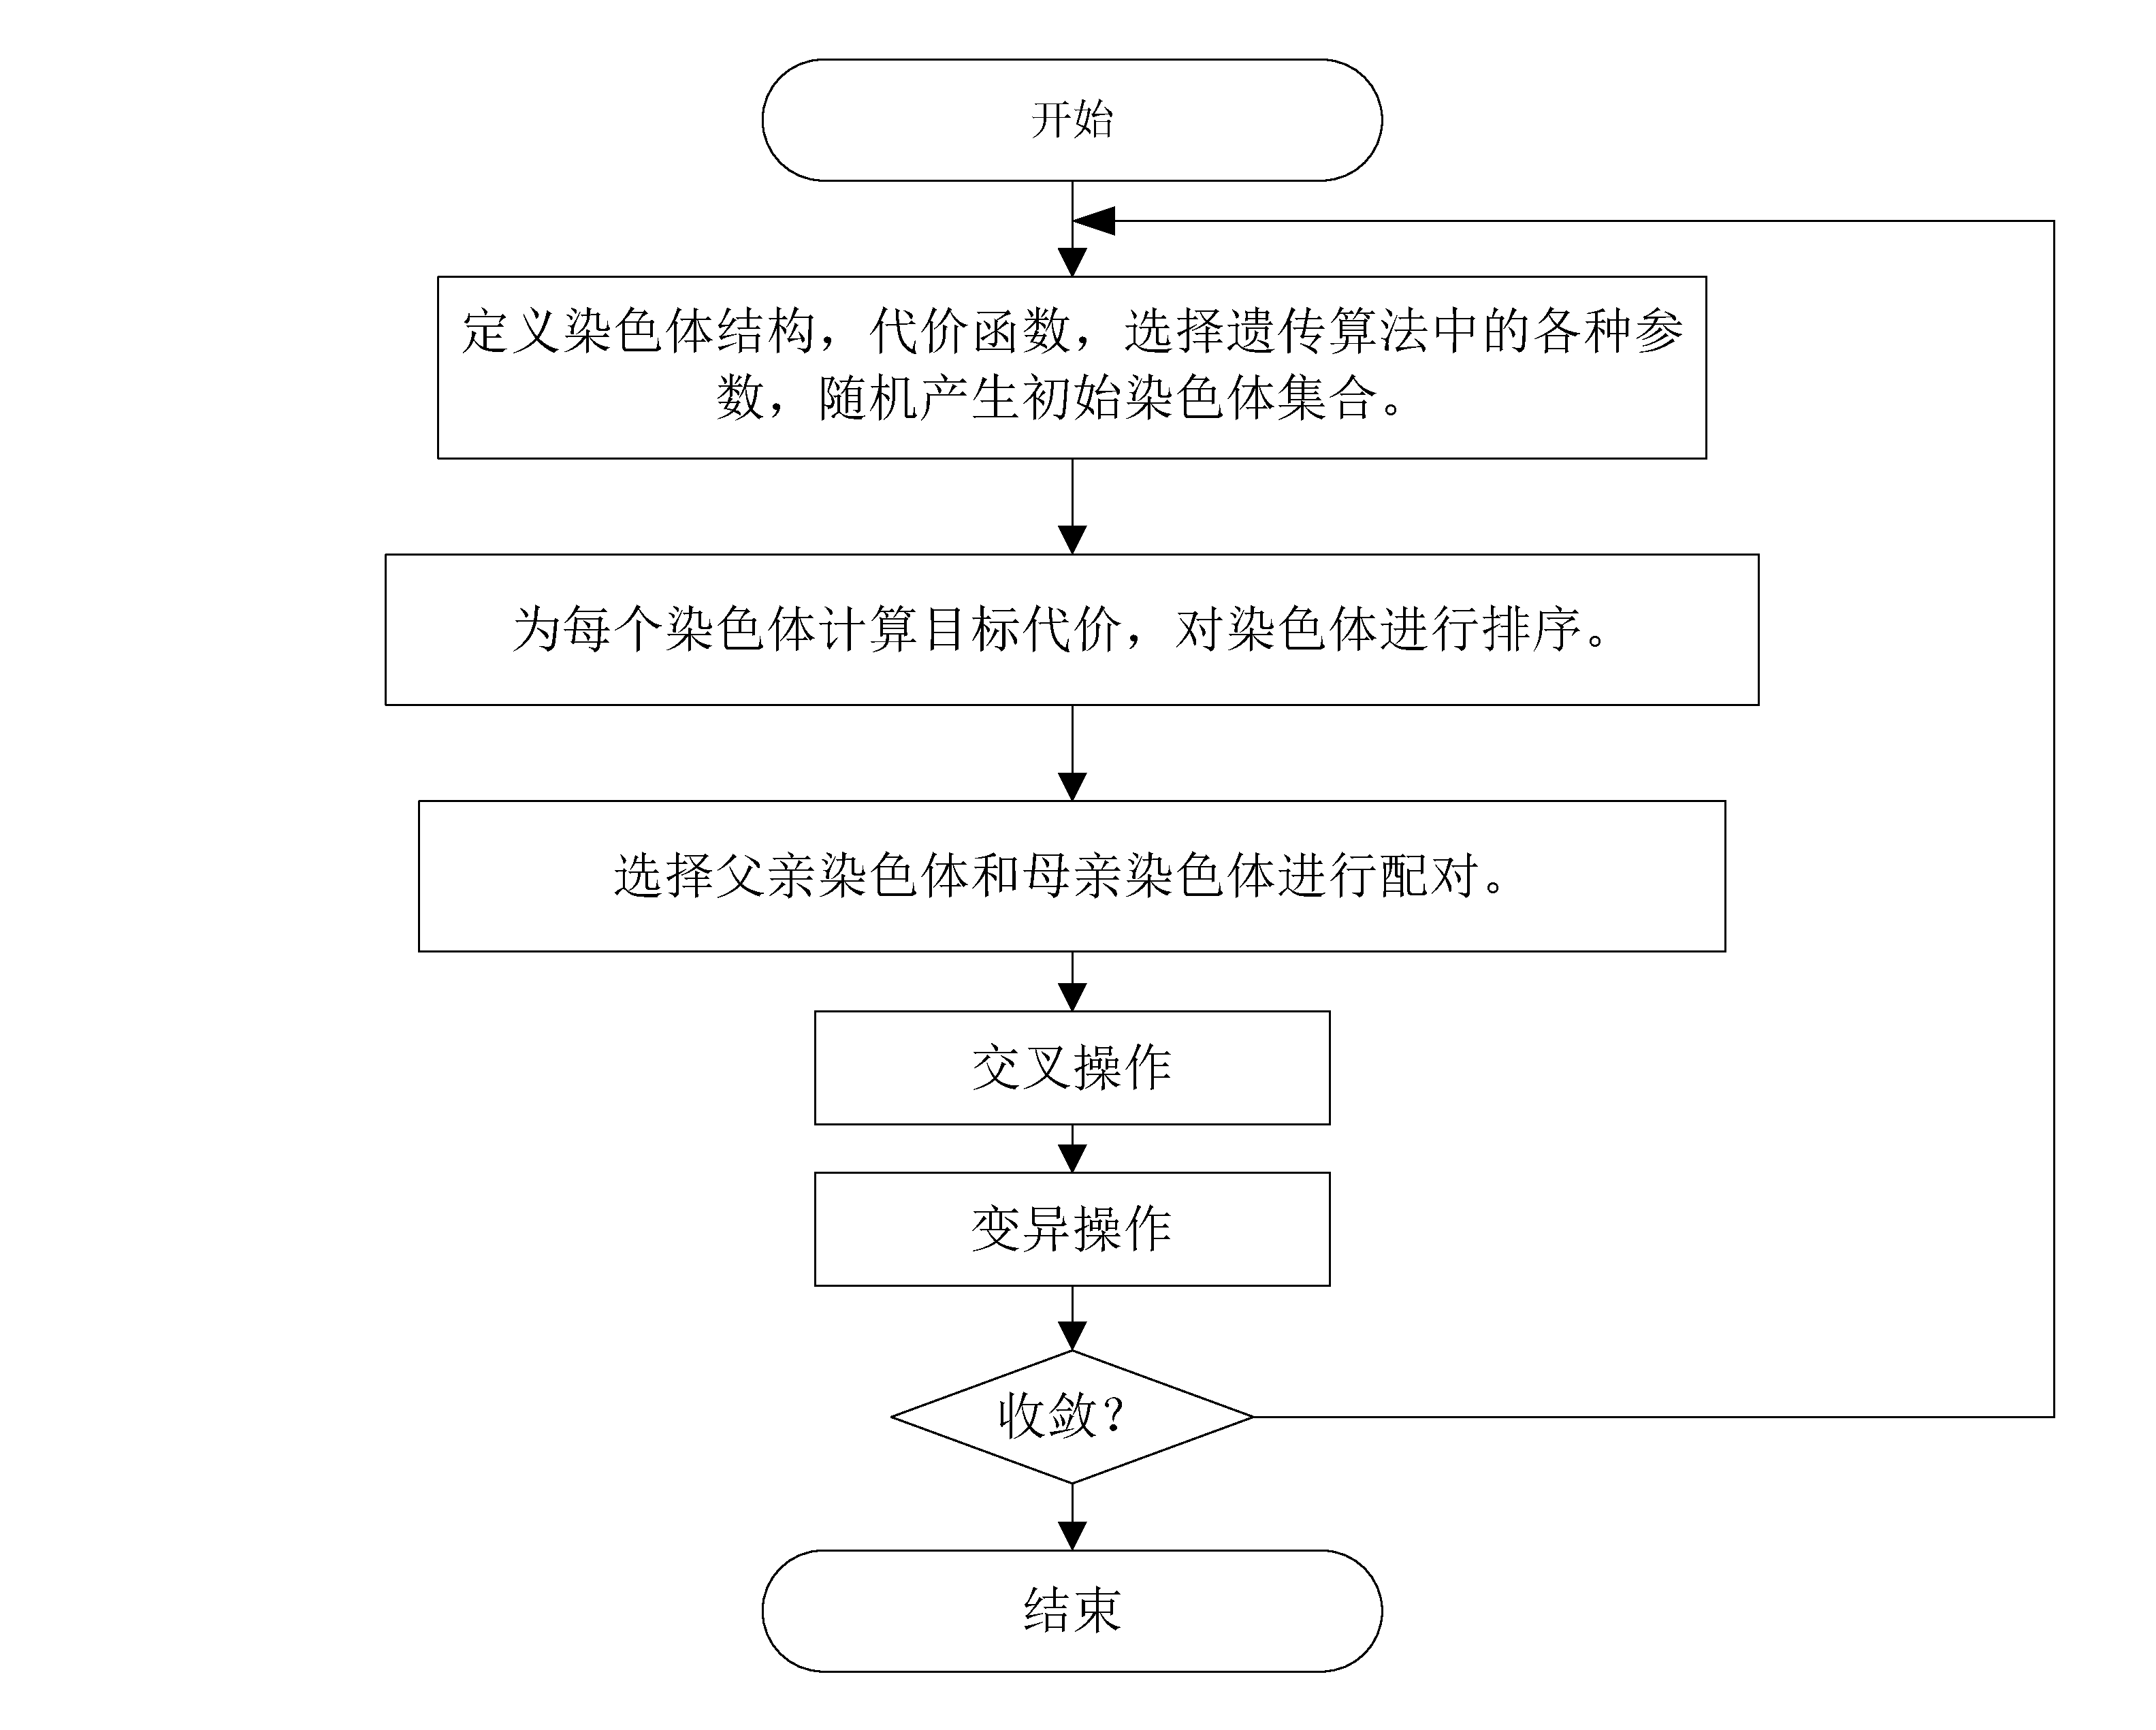
\includegraphics[width=0.8 \textwidth]{figures/GAprocess.pdf}}
\end{center}
\caption{{\footnotesize{GA算法流程图}}}
\label{IterNum}
\end{figure}
\subsubsection{染色体结构}

假设业务数量为$|D|$,初始染色体集合大小为$POP$,集合$C$表示染色体种群集合,$C_j$表示第$j$($j \in [1:POP]$)号染色体,$C^i_j=k,k \in [1:K]$表示在第$j$号染色体中,业务$i$选择了第$k$条备选路径,$C^i_j=0$表示业务$i$被阻塞(在辅助图$G_a(V_a,E_a)$上路由),不占用链路资源,$|p^i_d|$表示业务$d$的第$i$ 条备选路的路径代价,$rp^i_d$ 表示路径$p^i_d$ 上的最小可用容量,$rp^i_d=min(r_e|e \in p^i_d)$,其中$e \in p^i_d$ 表示路径$p^i_d$上的边,$r_e$ 表示此边$e$ 上的剩余容量。
\subsubsection{初始可行解的生成}
可行解表示满足容量约束的解,为了使得遗传算法有效,初始解的质量很重要,产生的初始解要尽量好,要有更多的业务要能加入网络中,而且保证业务的路径代价较小,本文采用一种简单的贪心算法来产生出初始可行解,算法如下\ref{alg:Framwork}所示:
\begin{algorithm}[htb]
\begin{algorithmic}[1]
\Require{$G(v,E)$:网络拓扑;$P$:备选路径集合;$C$:未初始化的染色体集合;}
\Ensure{$C$:可行染色体集合;}
\For{each $c_j \in C$}
\For{each $c^d_j \in c_j$ }
\State {$c^d_j\leftarrow k^d_j$,其中$k^d_j$为1到K之间的随机值,随机选择一条备选路}
\EndFor
\State {对染色体中的的每个业务需求按照值$\frac{bw_d}{\sqrt{|p^{k^d_j}_d|}}$}进行降序排序。
\For{each $c^d_j \in c_j$ }
\If{$rp^{k^d_j}_d>=bw_d$}
\State 加入路径$p^{k^d_j}_d$到网络,更新网络链路容量。
\Else
\State {$c^d_j \leftarrow 0$}
\EndIf
\EndFor
\EndFor
\end{algorithmic}
\caption{初始可行解产生}
\label{alg:Framwork}
\end{algorithm}

对每一个染色体,算法随机地为每个业务选择备选路径标号,但是这样选择出来的路径集合有可能会超过网络链路的容量限制,从而使得解变得不可行,要得到可行解,必须从解中剔除一部分业务,使得他们阻塞,本文使用一种启发式策略来确定需要剔除的业务,一方面,要使得目标函数变小,那些流量需求较大的业务应该优先被加入到网络中,但是。另一方面,如果大流量的业务的路由代价很大,经过了一条很长的路径,就会大量地浪费网络中的链路容量资源。所以算法对当前染色体$j$中的业务和其路径按照$\frac{bw_d}{\sqrt{|p^{k^d_j}_d|}}$ 的值进行排序,其中${bw_d}$ 代表当前业务$d$所需要的流量大小,$|p^{k^d_j}_d|$代表集合$P_d$ 中的第${k^d_j}$条路径的代价大小,观察目标函数,目标函数是最小化路由代价,而$\frac{bw_d}{\sqrt{|p^{k^d_j}_d|}}$较大意味着较大的流量经过较小代价的链路进行路由,这种路由是很理想的,尽量节省网络的链路使用资源的同时,又减小了总体目标函数,所以这个比例值是对业务路由优劣程度的较好评价。算法按照比例值排序的结果依次尝试将路径$p^{k^d_j}_d$加入到网络中,如果$rp^{k^d_j}_d>=bw_d$,表示路径经过的链路有足够的容量来容纳这一业务,所以加入业务到网络中,并且更新网络的链路容量大小,反之,如果$rp^{k^d_j}_d<bw_d$,这个业务选择这一条路径会超过网络链路的容量限制,于是这条业务被阻塞,染色体中的相应基因位置被设置为0。我们重复上面的过程$POP$次,就得到一个初始可行染色体集合$C$。
\subsubsection{评价}

评价过程对每一个染色体计算其相应的目标效用函数值,并且对染色体按照效用函数值进行降序排序,由于遗传算法中的交叉和变异步骤可能会产生不可行的染色体解(链路容量超限),我们把这样的染色体评价为一个很大的代价(INF),从而在选优时被排除掉。我们把排序好的染色体分为三组:

精英染色体集合:目标值排在最前面的$\alpha$个染色体构成精英染色体集合$A$,精英染色体将直接保留到下一轮迭代,而且精英染色体可以产生后代。

次优染色体集合:精英染色体后的$\beta$个染色体构成次优染色体集合$B$,次优染色体集合中的染色体不会直接保留到下一轮,但是他们可以和精英染色体进行交叉产生后代。

劣等染色体集合:最后剩余的$\gamma$个染色体构成劣等染色体集合$G$,由于其目标函数值一般较大,其选路策略不可取,算法直接扔掉这一部分劣等染色体,不允许劣等染色体产生后代。
\subsubsection{交叉}
交叉过程从精英染色体集合中$A$中随机选取一个染色体$c_i \in A$作为父亲,从精英染色体集合和较优染色体集合的并集$A \cup B$ 中随机选取一个染色体$c_j \in A \cup B$ 作为母亲,将$c_i$ 和$c_j$进行均匀交叉得到新的染色体$s$,均匀交叉的过程是,对$s$的每一个基因点位以$\%50$的几率选择继承父亲或者母亲的相应点位的路径选择。重复以上过程$\beta$ 次,从而产生$\beta$个新的子染色体。
\subsubsection{变异}
变异过程采用随机变异,随机在集合$A \cup B$中选取$\gamma$条染色体,对某一选定的染色体$c_j \in A \cup B$,随机选取$m$个业务基因点位,进行变异,将当前已经选择的路径编号随机改变为备选路集合中的另外一个值,由于变异过程是为了提高算法的的搜索空间,避免算法陷入局部最优解,但是实际实验过程中发现如果$M$和$m$值设置较大,可能使得算法收敛较慢,因为大量的变异可能会导致较优秀的可行解变成不可行,因此会丢掉这些优秀的解,因此实验中$m$的值设置得较小。
\subsubsection{终止条件}
假设第前$k$次迭代找到的最优解为$B^*$,第k+1次迭代找到最优解为$b_{k+1}^*$,如果$b_{k+1}^*<B^*$,那么就更新$B^*=b_{k+1}^*$,如果连续迭代$L$次,$B^*$都不被更新,则判定算法收敛,算法停止。
\subsection{基于GPU的并行遗传算法设计}
\subsubsection{并行评价算法设计}
遗传算法中最消耗时间的部分是染色体评价部分,由于需要评价大量的染色体,评价每个染色体都需要大量计算开销,但是幸运的是遗传算法具有天然的并行性,每个不同的染色体评价可以并行执行,更进一步,每个染色体中的不同基因的计算也可以并行执行,这样并行粒度是达到$|POP|\cdot|D|$。在具体介绍并行算法之前,我们先引入一些符号,如下:

染色体(chromosomes)相关符号:$C$表示染色体种群集合,$c_j$表示第$j$个染色体,$c^d_i$表示第$i$个染色体的第$d$个基因位置。

备选路径(paths)相关符号:$P$为所有业务的备选路径组成的集合,$P_i$表示第$i$业务的所有备选路径集合,$p_i^k \in P_i$表示集合$P_i$中的第$k$条路径。

业务带宽(bandwidth,bw),$bw_i$表示第$i$个业务需要的带宽大小。

链路流量(flow,f),$f_e$表示链路$e$上占用的流量大小。

链路单位代价(weight,w),$w_e$表示链路$e$上的代价。

链路流量(capacity,ca),$ca_e$表示链路$e$上的容量大小。

共享内存中间数组(shared,sh),$sh_e$表示链路$e$上的总代价。

目标函数值数组(objectives,ob),$ob_j$表示第$j$个染色体对应的目标函数值。

\begin{algorithm}[t]
\begin{algorithmic}[1]
\Function{evaluate}{$C$,$P$,$bw$,$w$,$ca$,$ob$}
\State {在block上分配大小为|E|的共享内存空间组成数组f,初始化数组f中的所有值为零。}
\State {$j \leftarrow$ block ID}
\State {$d \leftarrow$ thread ID}
\State {$k \leftarrow c_j^d$}
\For {$e \in p_d^k$}
\State {$atomicAdd(f_e,bw_d)$}
\EndFor
\State{调用block线程同步函数\_\_syncthreads()}
\State {在block上分配大小为|E|的共享内存空间组成数组sh,初始化数组sh中的所有值为零。}
\State{$e \leftarrow thread ID$}
\If {$f_e<ca_e$}
\State{$sh_e \leftarrow f_e\cdot w_e$}
\Else
\State{$sh_e \leftarrow INF$}
\EndIf
\State{调用block线程同步函数\_\_syncthreads()}
\State{$s \leftarrow |E|$}
\While{s>1}
\If{e<s/2}
\State{$sh_e \leftarrow sh_e+sh_{(e+(s+1)/2)}$}
\EndIf
\State{调用block线程同步函数\_\_syncthreads()}
\State{$s \leftarrow (s+1)/2$}
\EndWhile
\State{$ob_j=sh_0$}
\EndFunction
\end{algorithmic}
\caption{kernel函数evaluate}
\label{evaluate}
\end{algorithm}

由于每个染色体的计算过程是独立的,算法为每一个染色体开辟一个block,一个block内部的第$d$号线程负责当前染色体上第$d$号业务的计算。算法 \ref{evaluate}展示了负责评价的kernel函数evaluate,算法一共可以分为两个部分:

第一,流量统计部分:算法需要对染色体进行可行性判断,也就是判断是否有链路的流量大小超过其容量大小,为此算法需要统计每一条边上的流量大小,我们在共享内存中开辟数组f用以统计流量,f数组被初始化为0。一个block中的每一个线程首先通过寻址备选路径集合找到业务选择的路径,
业务每经过一条链路都需要占用链路上的容量,所以如果路径经过了链路$e$,$f_e$就需要加上业务的流量大小,block中的每一个线程都会遍历业务所选择的路径,对$f$数组进行加法操作,但是多个线程可能同时对f数组中的同一个地址进行加法操作,这不是同步安全的,所以算法使用atomicAdd操作进行原子加法,避免同步问题。
当线程完成对$f$数组的统计之后,必修进行同步(syncthreads()),同步操作保证block内部的所有线程执行到同一步骤,也就是先统计完成的线程必修等待其他统计线程也执行完成后才能继续执行,因为只有所有线程都完成对$f$数组的加法操作,$f$数组的值才完整,才能够进行下一步操作。

第二,效用函数计算部分:效用函数为链路的代价和,算法需要先计算每一条链路上的代价值,我们在共享内存中开辟数组$sh$来对每一条边的代价进行统计,每一个线程负责对一条链路代价的计算。比如,线程$e$负责第$e$条边的代价计算,线程$e$首先判断链路的流量是否溢出($ca_e<f_e$),如果溢出则说明此染色体表示的解不可行,设置$sh_e$为$\infty$,这使得这个染色体在排序时会被归类到劣等集合,从而在下一次迭代之前被剔除掉。反之,如果$f_e \le ca_e$,则说明链路容量足够,链路的代价为$f_e \cdot w_e$,设置$sh_e$为$f_e \cdot w_e$。和$f$数组的统计一样,当线程统计完成$sh_e$之后,也需要进行同步操作,等待其他线程完成统计。$sh_e$数组计算完成之后,还需要把$sh_e$中的值进行加和才能得到效用函数的值,为了充分利用GPU多线程,算法最后进行并行规约操作(20-26行)进行求和,for循环中每次将后一半的$sh$数组加到前一半,规约过程中必修进行同步(syncthreads()),以保证加法过程计算完整,最终求和值规约到$sh_0$,将$sh_0$中的值写入到$ob$数组中。
\begin{figure}
\begin{center}
{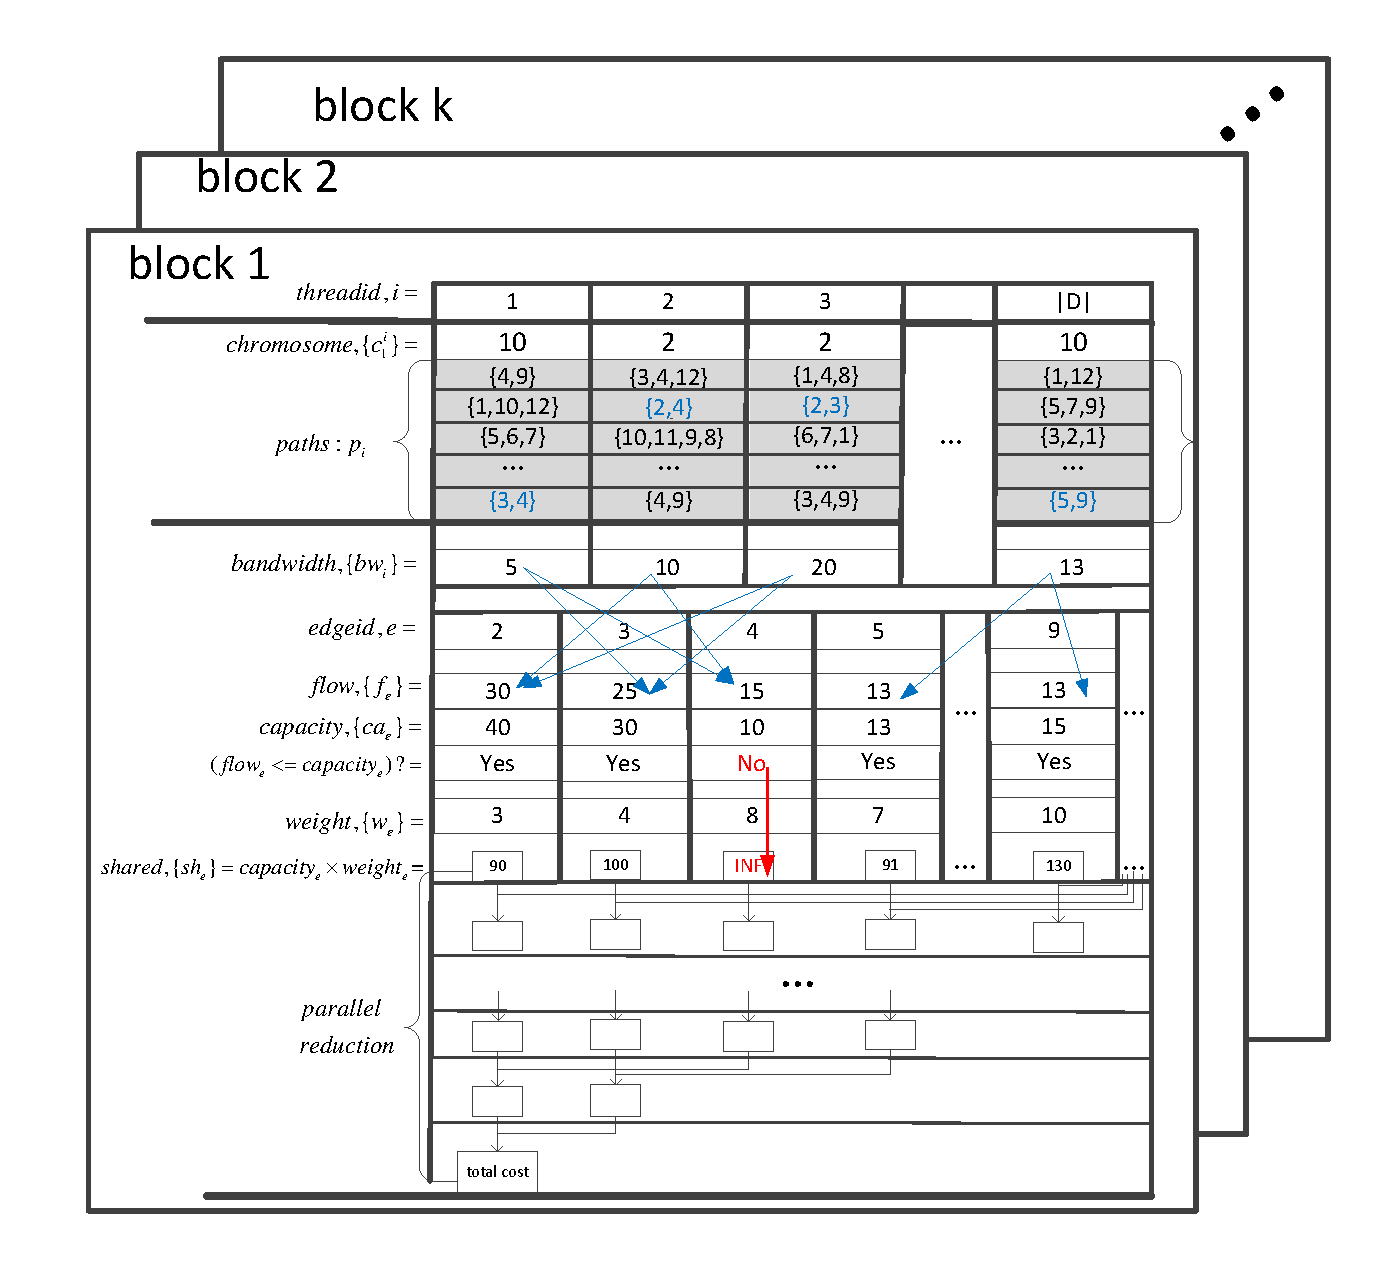
\includegraphics[width=1 \textwidth]{figures/GPUfitness.pdf}}
\end{center}
\caption{{\footnotesize{GPU并行评价示例}}}
\label{fitness}
\end{figure}

图\ref{fitness}为GPU上并行评价算法的一个具体例子,图中被标位蓝色的数组表示业务选择的路径,蓝色的箭头表示流量统计时的加法操作,红色箭头表示链路流量超过链路容量,使得链路代价被设置为$\infty$。
\subsubsection{并行排序,变异与交叉}
由于遗传算法中最消耗时间的部分是评价部分,本设计中对其他部分的并行步骤采用较简单的算法。在评价部分结束后,需要对所有的染色体按照效用函数的大小降序排序,本设计采用CUDA提供的Thrust\citing{Thrust}中提供的排序函数对GPU上的染色体进行排序,Thrust是基于标准模板库(STL)的CUDA C++模板库,Thrust为程序员提供常见的CUDA算法库,能够减少程序员工作量并且提高应用程序效率,Thrust库中的排序函数已经针对GPU架构做了很好得优化,所以本文不在对排序部分进行优化,排序函数细节可参考NVDIA官方文档\citing{Thrust}。

交叉过程分为父母选取和交叉计算两个kernel,父母选取过程并行地选取$\beta$对父母,每个线程负责选取一对父母,并且将选取的父母下标记录到$father$和$mother$数组中,父母选取GPU计算示意图如下图\ref{pp}所示:
\begin{figure}
\begin{center}
{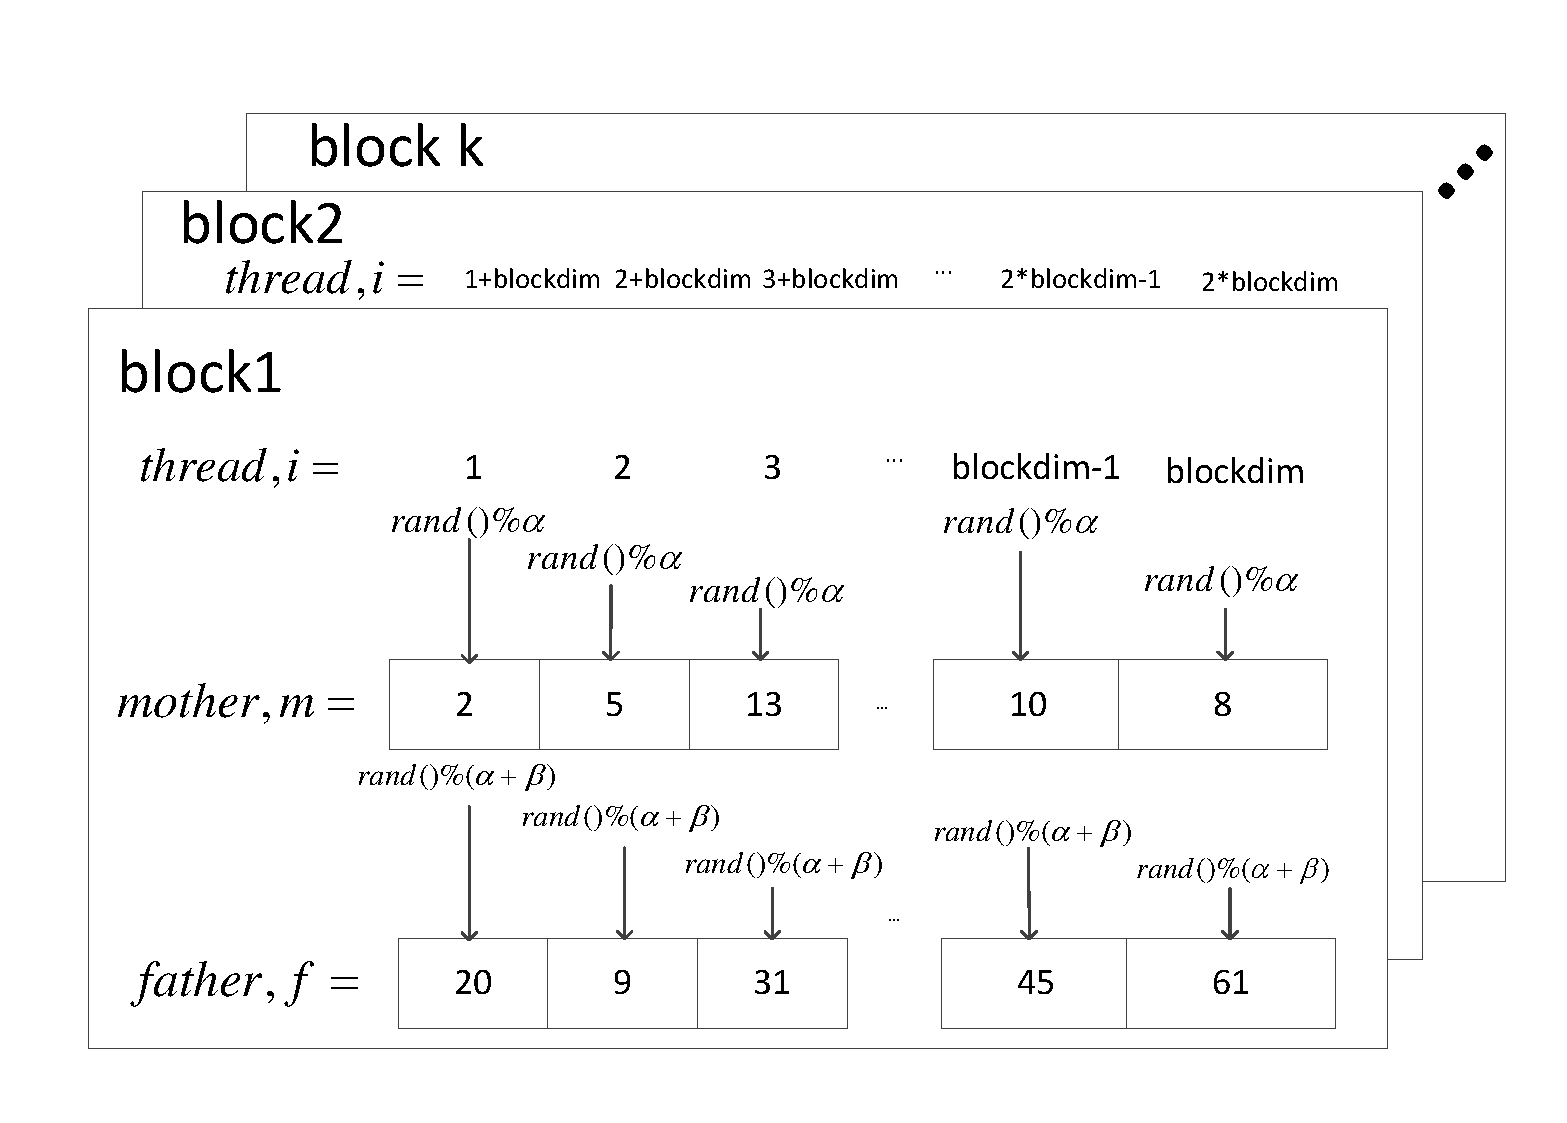
\includegraphics[width=0.8\textwidth]{figures/GPUchoose.pdf}}
\end{center}
\caption{{\footnotesize{GPU并行父母选取过程}}}
\label{pp}
\end{figure}
每个线程进行两次随机,$mother$标号只能在前$\alpha$个精英染色体中选取,$father$表号的选取在前$\alpha+\beta$ 中选取,这样既能够给予精英染色体更大的繁殖几率,也可以保证解的搜索空间变化足够大,避免陷入局部最优值。

父母选取过程结束后,在GPU端记录了所选取的$mother$和$father$数组,$mother$和$father$数组将用于交叉部分的计算,交叉部分的并行粒度更高,其中每个基因点的计算都是并行执行的,如下图 \ref{cross} 所示:
\begin{figure}
\begin{center}
{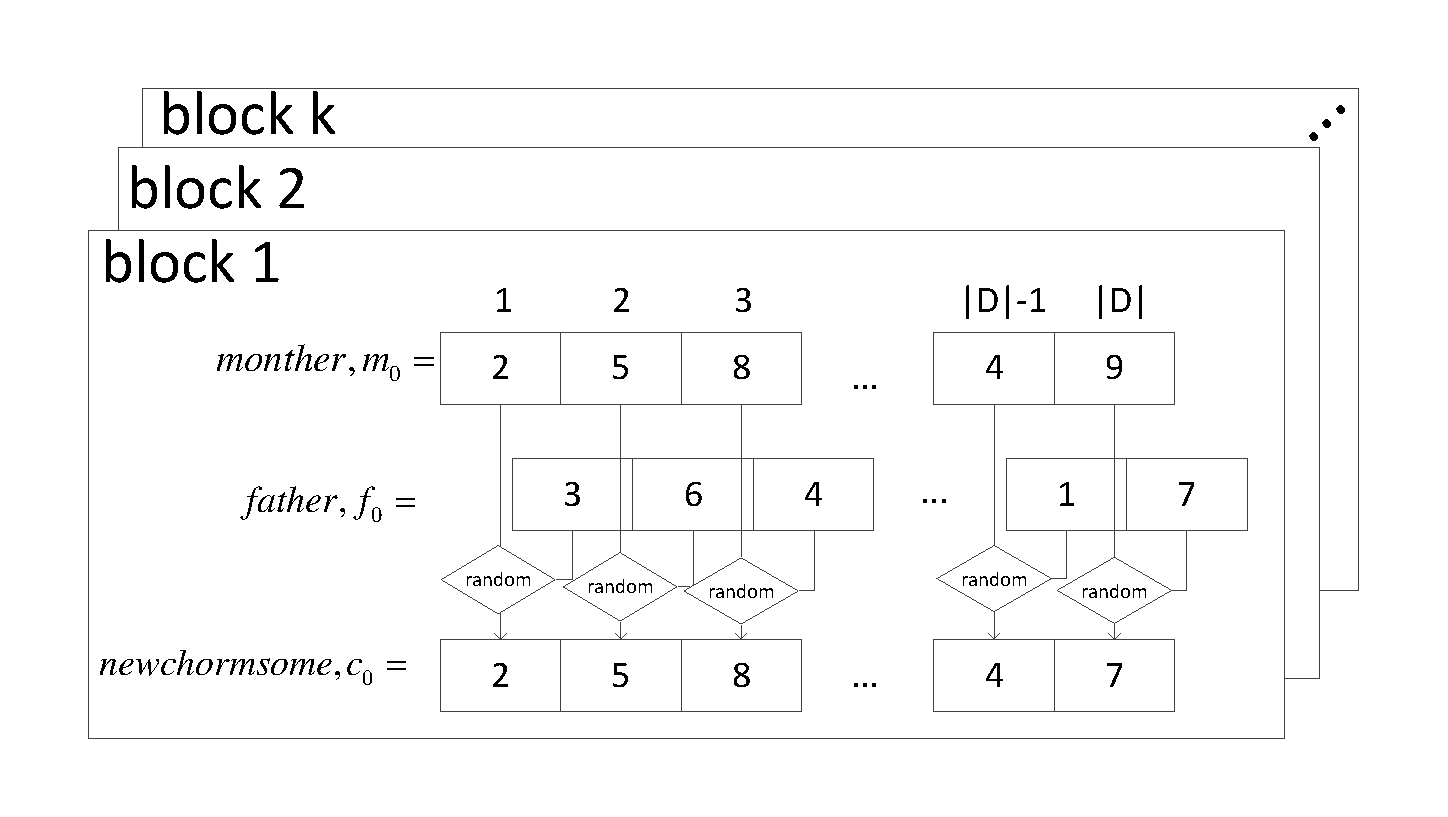
\includegraphics[width=0.8\textwidth]{figures/GPUcross.pdf}}
\end{center}
\caption{{\footnotesize{GPU并行均匀交叉过程}}}
\label{cross}
\end{figure}
每个block负责一个新染色体的生成,通过之前的分析,一共需要生产$\beta$个新的染色体,所以GPU端一共需要分配$\beta$ 个block,其中每一个block中有|D|个线程来同时负责随机从$mother$和$father$的相应点位选择一个来作为新染色体相应点位的值,如前所说采用均匀交叉策略,选择父亲母亲遗传基因的概率都是50\%,这样block内部的并行度达到$|D|$,总的并行粒度达到$\beta \cdot |D|$。

最后,对于变异部分,我们一共开辟$\gamma$个线程,每个线程随机在$A\cup B$集合中选取一个染色体,并随机选取$m$个点位进行变异,并行粒度为$\gamma$。
\section{基于拉格朗日的优化算法设计}

GA-PTEA算法虽然简单,但是其具有以下缺点:第一,需要事先计算大量备选路径,不能很好地适应网络的动态变化,一旦网络链路发生变化,又要重新计算备选路径。第二,遗传算法从开始到收敛需要大量的迭代次数,虽然经过GPU加速,但是由于收敛缓慢,仍然需要大量的计算时间。第三,遗传算法容易陷入局部最优解。

本节采用基于拉格朗日松弛的模型来解决业务量工程问题,并根据这个模型设计出并行算法LR-PTEA(Lagrange relaxing based parallel traffic engineering algorithm),LR-PTEA相对与GA-PTEA有以下优点:第一,LR-PTEA能够快速收敛。第二,LR-PTEA求得的解大大优于GA-PTEA。第三,LR-PTEA不需要事先产生备选路径,业务路由是实时计算出来的。
\subsection{基于拉格朗日松弛的模型}
在模型(\ref{Obj2},\ref{FlowConv},\ref{Capcon})中,网络容量约束(式子 \ref{Capcon}),把所有的路由变量联系到一起,因为这些变量的取值必修保证每一条链路上占用的流量小于链路的容量大小,正是由于存在链路容量约束,每个业务的路由选取才变得不相互独立,但是要利用GPU 的并行特性,需要寻找独立计算的可能性,因此,本文采用拉格朗日松弛方法,把一个业务量工程问题分解成一批业务的路由计算问题,而这些业务的路由计算问题是相互独立的,很适合并行计算。

将模型(\ref{Obj2},\ref{FlowConv},\ref{Capcon})中的网络容量约束松弛进目标函数得到如下拉格朗日子问题:
\begin{equation}\label{LagProb}
\begin{split}
L(\mathbf{\lambda})= min\sum\limits_{d \in D}\sum\limits_{(i,j) \in E_b} w_{ij}x_{ij}^d bw_d+ \\ ~~~~~\sum\limits_{(i,j) \in E_b}\lambda_{ij}(\sum\limits_{d \in D} x_{ij}^d bw_d-c_{ij})
\end{split}
\end{equation}
其中 $\lambda_{ij}$ 表示链路 $(i,j)$的拉格朗日乘子。

表达式(\ref{LagProb})还可以表示为:
\begin{equation}\label{Lagprob1}
L(\mathbf{\lambda})= min\sum\limits_{d \in D}\sum\limits_{(i,j) \in E_b} (w_{ij}+\lambda_{ij})x_{ij}^dbw_d -\sum\limits_{(i,j) \in E_b}\lambda_{ij}c_{ij}
\end{equation}
受限于:
\begin{equation}\label{FlowConv2}
\begin{split}
\sum\limits_{(i,j) \in E_b} x_{ij}^d - \sum\limits_{(j,i) \in E_b} x_{ji}^d
=\begin{cases}
1 & \text{if $i = s_d$}\\
-1 & \text{if $i = t_d$} \\
0 &{otherwise}
\end{cases}
\\~~~~~~~~\forall i\in V_b, \forall d\in D
\end{split}
\end{equation}
拉格朗日子问题的目标函数中的$\sum_{(i,j) \in E_a}\lambda_{ij}c_{ij}$这一项,不随着拉格朗日乘子的变化而变化,本文将其作为常数项而丢掉不讨论,丢掉$\sum_{(i,j) \in E_a}\lambda_{ij}c_{ij}$ 这一项后,拉格朗日子问题的目标函数中只含有代价部分 $w_{ij}+\lambda_{ij}$和$x_{ij}^d bw_d$的乘积。注意到,$\sum_{(i,j) \in E_a} (w_{ij}+\lambda_{ij})x_{ij}^d bw_d$表示业务$d$的路由代价,因此,拉格朗日子问题的目标函数是最小化所有业务的路由代价总和,观察这个子问题的约束,我们发现,每一个约束都只含有一个和业务需求相关的变量,所以,这个拉格朗日子问题可以被分解成一系列独立的最短路径问题(每个业务需求对应于一个最短路问题),只是这些最短路径问题的链路代价发生了改变,链路代价变得和拉格朗日乘子 $\mathbf{\lambda}$ 相关,也就是说给定一个拉格朗日乘子$\mathbf{\lambda}$,我们可以将拉格朗日子问题看成一批单业务的最短路径问题,我们可以通过并行地计算一系列的最短路径来解决这个拉格朗日子问题。

因为把容量约束松弛进效用函数中后,不会增加目标函数的值, $L(\mathbf{\lambda})$成为原问题最优目标函数值的下界,$z^* \ge L(\mathbf{\lambda})$,为了得到最紧的的下界值,我们要解决以下这个优化问题:
\begin{equation}\label{dual}
L^*(\mathbf{\lambda^*}) = maximize_{\mathbf{\lambda}}L(\mathbf{\lambda})
\end{equation}
~~受限于: (\ref{FlowConv2})
\vskip 0.2cm

以上的这个优化问题也被称为原来业务量工程问题(式子\ref{Obj2},\ref{FlowConv},\ref{Capcon})的对偶问题 \citing{NetworkFlow},其中$\mathbf{\lambda^*}$ 表示最优拉格朗日乘子,为了得到最优乘子$\mathbf{\lambda^*}$,可以使用次梯度优化算法来解决,次梯度优化计算时,第一次先初始化乘子 $\mathbf{\lambda}^0$, 然后通过以下过程进行迭代求解:
\begin{equation}\label{iter}
\mathbf{\lambda}_{ij}^{(k+1)} =\mathbf{\lambda_{ij}}^{(k)}+\theta_{k} g^{(k)}= \mathbf{\lambda_{ij}}^{(k)} + \theta_k[(\sum\limits_{d \in D}x_{ij}^d bw_d- c_{ij})]^+
\end{equation}
其中, $\mathbf{\lambda}_{ij}^{(k)}$表示第$k$次迭代的对应于边$(i,j)$的拉格朗日乘子, $g^{(k)}$是$L(\mathbf{\lambda})$ 对$\mathbf{\lambda}^{k}$的任意一种次梯度,$\theta_k$ 表示第$k$次的迭代的步长,标记$[\alpha]^+$ 表示$\alpha$中符号为正的部分,也就说$[\alpha]^+=max(\alpha, 0)$,从表达式Eq. (\ref{iter})可以看出来如果链路$(i,j)$ 上的流量总和超过链路$(i,j)$上的容量,链路$(i,j)$ 上的$\lambda_{ij}^k$拉格朗日乘子会增加,也就是表示一些业务流量需要从链路$(i,j)$上移除,另外,为了避免产生负权重的链路代价,当链路容量大于其上的流量时,我们并不去减小此链路$(i,j)$上的$\lambda_{ij}^k$。
根据以上讨论,我们给出基于拉格朗日乘子法的并行路由优化算法的框架,如图\ref{lpl}所示,LR-PROA主要包括以下步骤:

步骤一,为$G_a(V_a, E_a)$ 初始化链路权重。

步骤二,计算所有业务的最短路径,其中路径计算任务被分配到GPU 进行并行计算。

步骤三,为了从当前计算出来的路径中得到原问题的优化目标函数值,对步骤二中计算出来的路径进行调整。

步骤四,更新链路权重,更新完毕后,如果停止条件不满足,则回到步骤二,进入下一轮迭代。LR-PROA 如果在连续$L$次成功的迭代后依然不能找到更优的全局解,则停止算法过程。
\begin{figure}
\begin{center}
{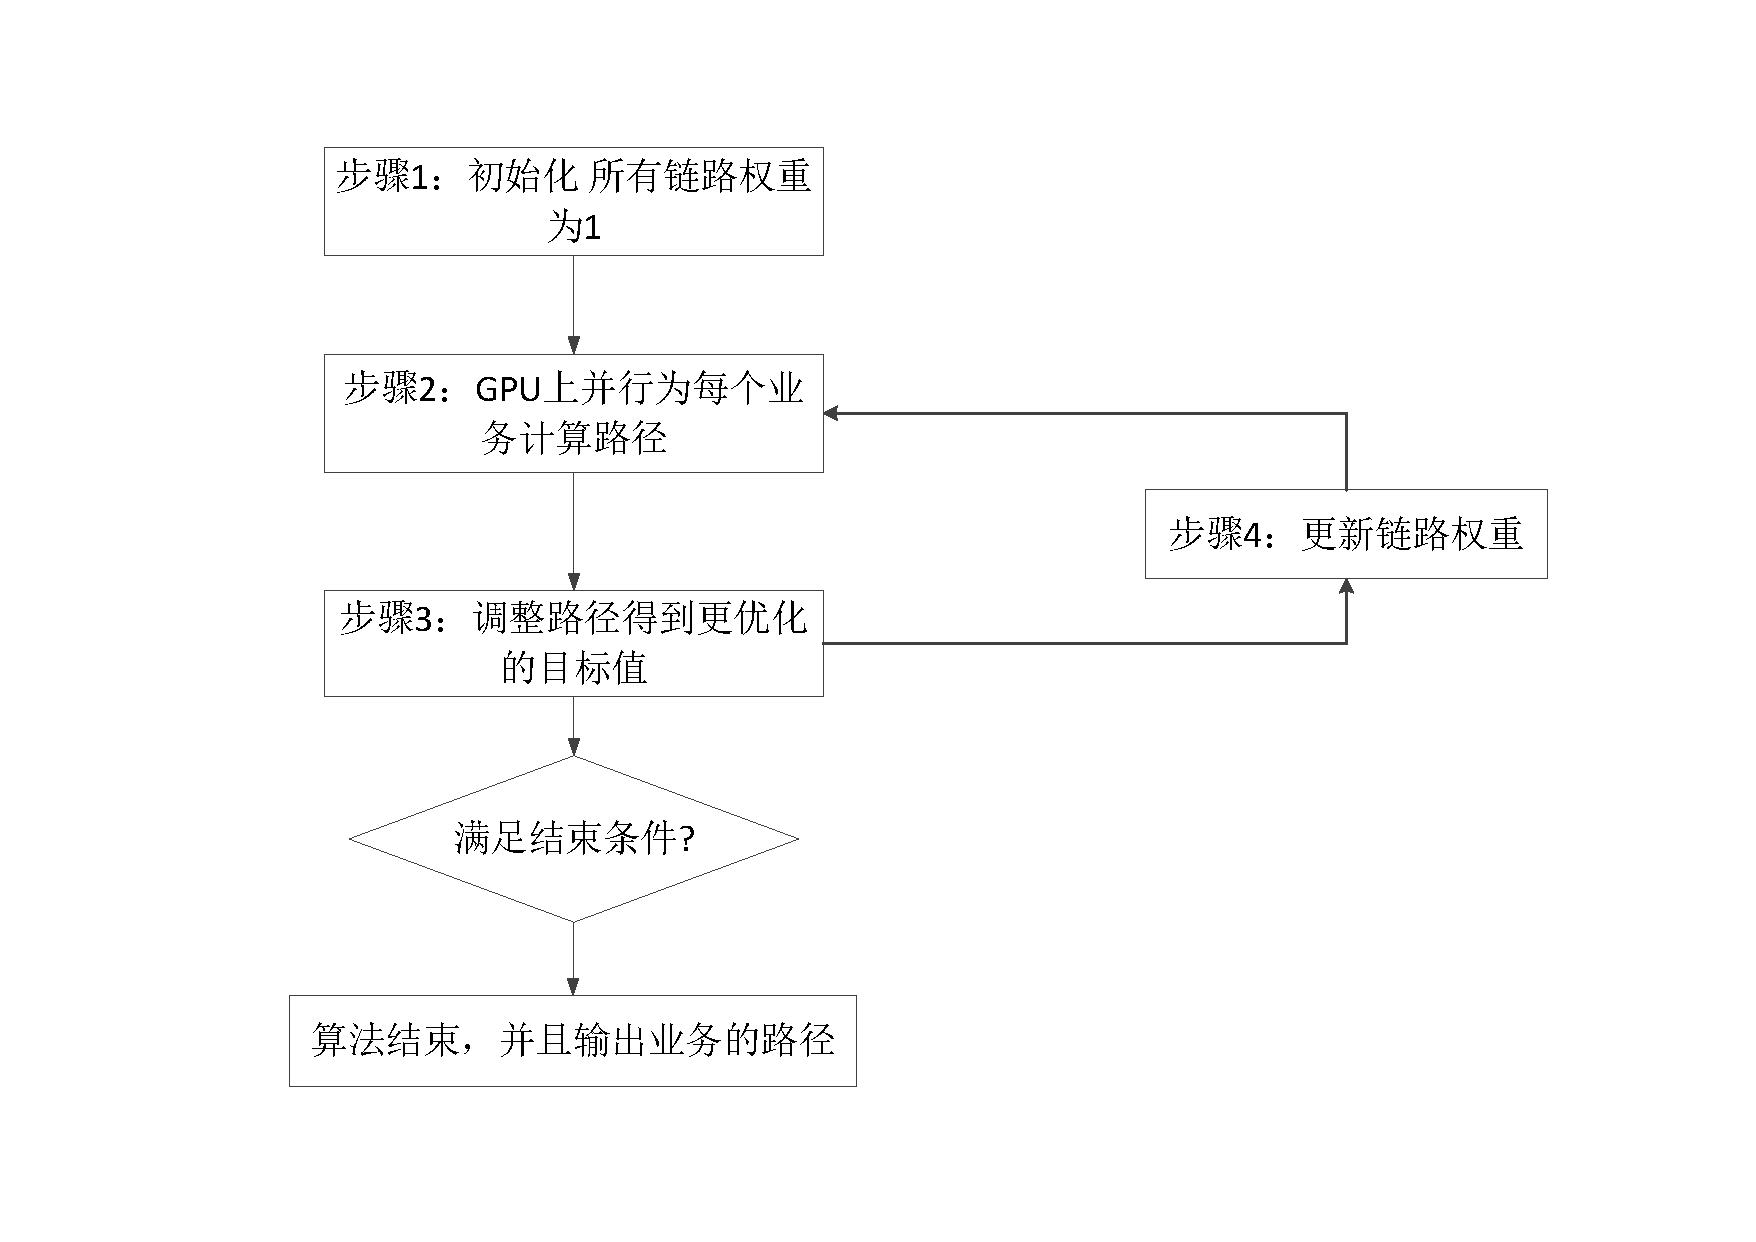
\includegraphics[width=0.8\textwidth]{figures/lagrange.pdf}}
\end{center}
\caption{{\footnotesize{LR-PROA算法流程图}}}
\label{lpl}
\end{figure}
\subsection{基于GPU的并行路由计算}
在每次迭代中,LR-PROA为每个业务 $d \in D$在图 $G_a(V_a, E_a)$中计算最短路径,显然,丢掉链路容量约束后,不同业务的最短路径计算可以独立在GPU上并行执行,但是,最短路算法的逻辑对于GPU来说太过复杂,GPU最初是被设计来做大规模的数值计算问题,其只实用于逻辑比较简单,但是数值计算量较大的任务,所以在GPU上直接开辟一个线程来计算一个业务的路径,不仅仅在计算上是低效的,而且这样的并行粒度也不能充分利用GPU 的大规模并行能力。为了充分提高最短路径的计算速度,LR-PROA 对最短路径算法进行并行化设计。
\begin{algorithm}[htb]
\begin{algorithmic}[1]
\Require
网络拓扑:$G(V, E)$;
源点:$s$;
\Ensure
从$s$开始到其他点的路径集合$P$;
\For {each node $v \in V$}
\State {$Dist[v] \leftarrow \infty$}
\State {$Pre[v] \leftarrow $ NIL}
\EndFor
\State {$Dist[s] \leftarrow 0$}
\State {$Mark \leftarrow 1$}
\While {$Mark > 0$}
\State {$Mark \leftarrow 0$}
\For{each link $(u,v) \in E$}
\If{$Dist[v]>Dist[u]+w_{uv}$}
\State {$Dist[v] \leftarrow Dist[u]+w_{uv}$}
\State {$Pre[v] \leftarrow u$}
\State {$Mark = 1$}
\EndIf
\EndFor
\EndWhile
\State {根据前驱数组$Pre$,重新构建最短路集合,输出路径到集合$P$}
\end{algorithmic}
\caption{{Bellman最短路算法}}
\label{Bellman}
\end{algorithm}
文章 \citing{SSP1}提出一种Dijkstra最短路径算法在GPU上的并行实现,但是从算法结构上分析,Dijkstra最短路径算法并不适应于并行算法的设计,所以Dijkstra最短路径算法在GPU上的实现不能得到很好的加速效果,为了期望得到更好的加速效果,LR-PROA 选择Bellman-Ford \citing{NetworkFlow}最短路算法来进行并行实现,Bellman-Ford最短路算法逐步地减小距离标记 $Dist[v],v\in V$,直到其收敛到真实的最短距离。Bellman-Ford算法过程如算法\ref{Bellman},其中 $Dist[v]$ 表示距离起点$s$到$v$的最短路径距离,$Pre[v]$ 表示点$s$到点$v$ 的最短路径上$v$ 的前驱节点,在初始化好了所有节点的距离数组和前驱节点数组之后,Bellman-Ford算法最多迭代 $|V|$ 次,每一次迭代算法松弛一次图$G(V, E)$ 中的所有的边(第10-11行)。Bellman-Ford 算法的算法复杂度为$(|V|\cdot |E|)$,他的复杂度高于Dijkstra最短路径算法的复杂度,但是,因为Bellman-Ford算法每次松弛边的操作都是独立无关的,通过为每一条边的松弛操作分配一个独立的线程执行,Bellman-For算法很容易在GPU 上实现并行化。
\begin{figure*}
\setlength{\belowcaptionskip}{-0.5cm}
\begin{center}
{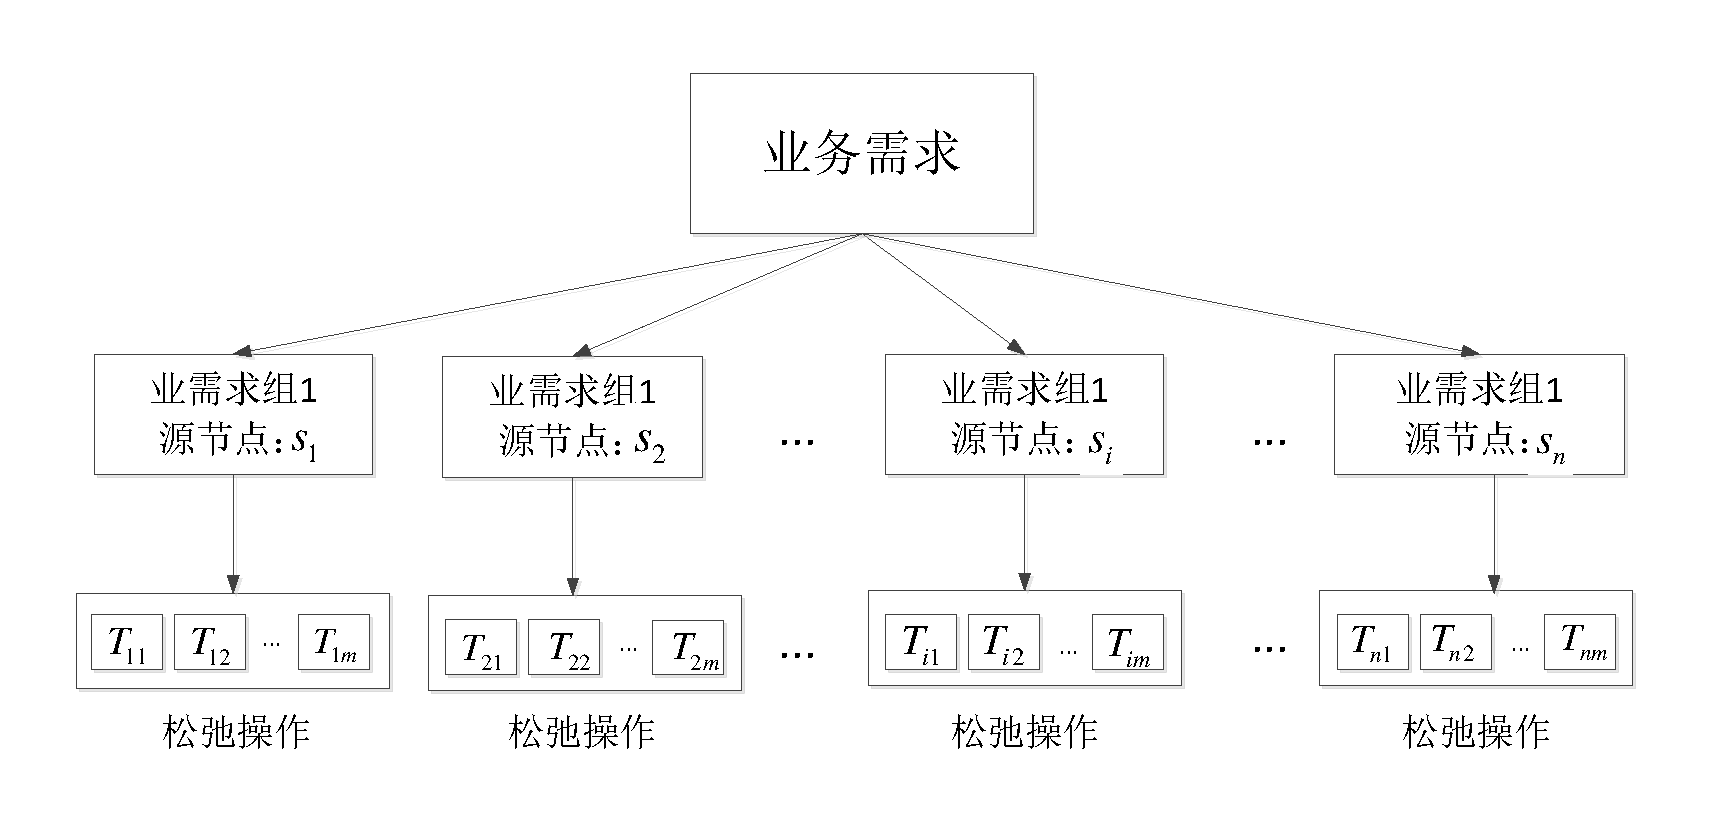
\includegraphics[width=1 \textwidth]{figures/paframework.pdf}}
\end{center}
\caption{{\footnotesize{并行业务计算框架}}}
\label{ParFramework}
\end{figure*}

图 \ref{ParFramework} 中显示了LR-PROA的最短路径计算的并行实现框架。首先,根据业务的源节点将业务分配成不同的组,使得每一组内的业务的源节点相同。我们假设第$i$个组的源节点为$s_i$。 然后,每一组的最短路径计算使用$m$个GPU 线程的并行bellman-ford算法进行计算,如图\ref{ParFramework}所示,线程$T_{i,j}$负责为对应于源点$s_i$的链路$e_{j}$ 进行松弛操作。因此总的并行执行的线程数是$m \times k$,其中$m$和$k$分别表示链路数目和组的数目。

在本文的最短路算法的并行实现中,每个block内部的线程都松弛同一条链路,比如,在图 \ref{GB} 中,集合$\{T_{1j}, T_{2j}, \cdots, T_{ij}, \cdots, T_{kj}\}$都在$block_j$上执行,其中 $T_{ij}$为对应源节点为$s_i$ 的链路$e_i$执行松弛操作,其中,我们设链路$e_i$的头节点和尾节点分别为$h_i$ 和$t_i$,可以看到,当这次迭代存在链路更新,那么标记$Mark$会被设置成1,这是为了优化算法的迭代次数,当某次迭代结束$Mark=0$ 则表示这次迭代没有边进行了更新操作,说明Bellman 算法已经提前结束,实验证明这一个优化可以大大地减小Bellman算法的迭代运行次数。
\begin{figure*}
\setlength{\belowcaptionskip}{-0.5cm}
\begin{center}
{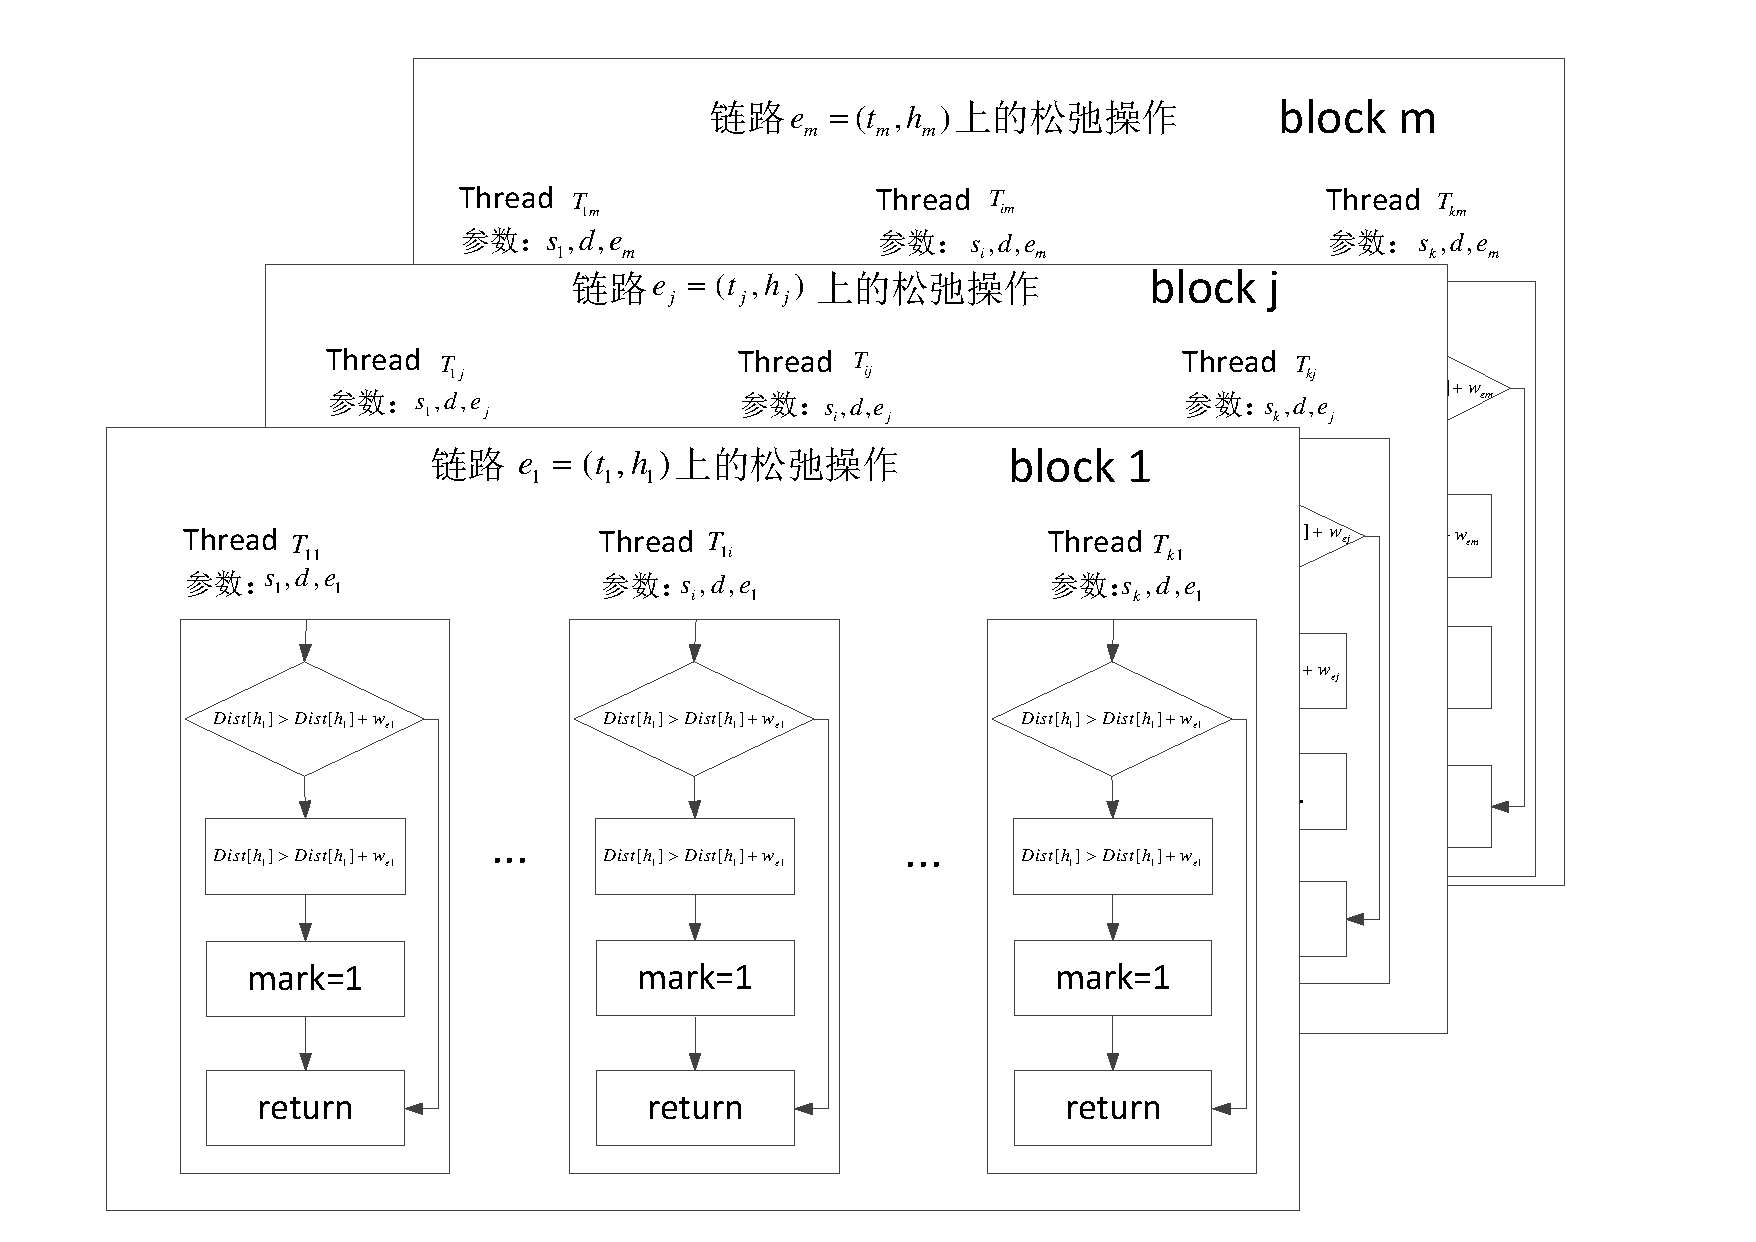
\includegraphics[width=1 \textwidth]{figures/GPUimpl.pdf}}
\end{center}
\caption{{\footnotesize{GPU上Bellman算法的实现}}}
\label{GB}
\end{figure*}

\begin{figure*}
\setlength{\belowcaptionskip}{-0.1cm}
\begin{center}
{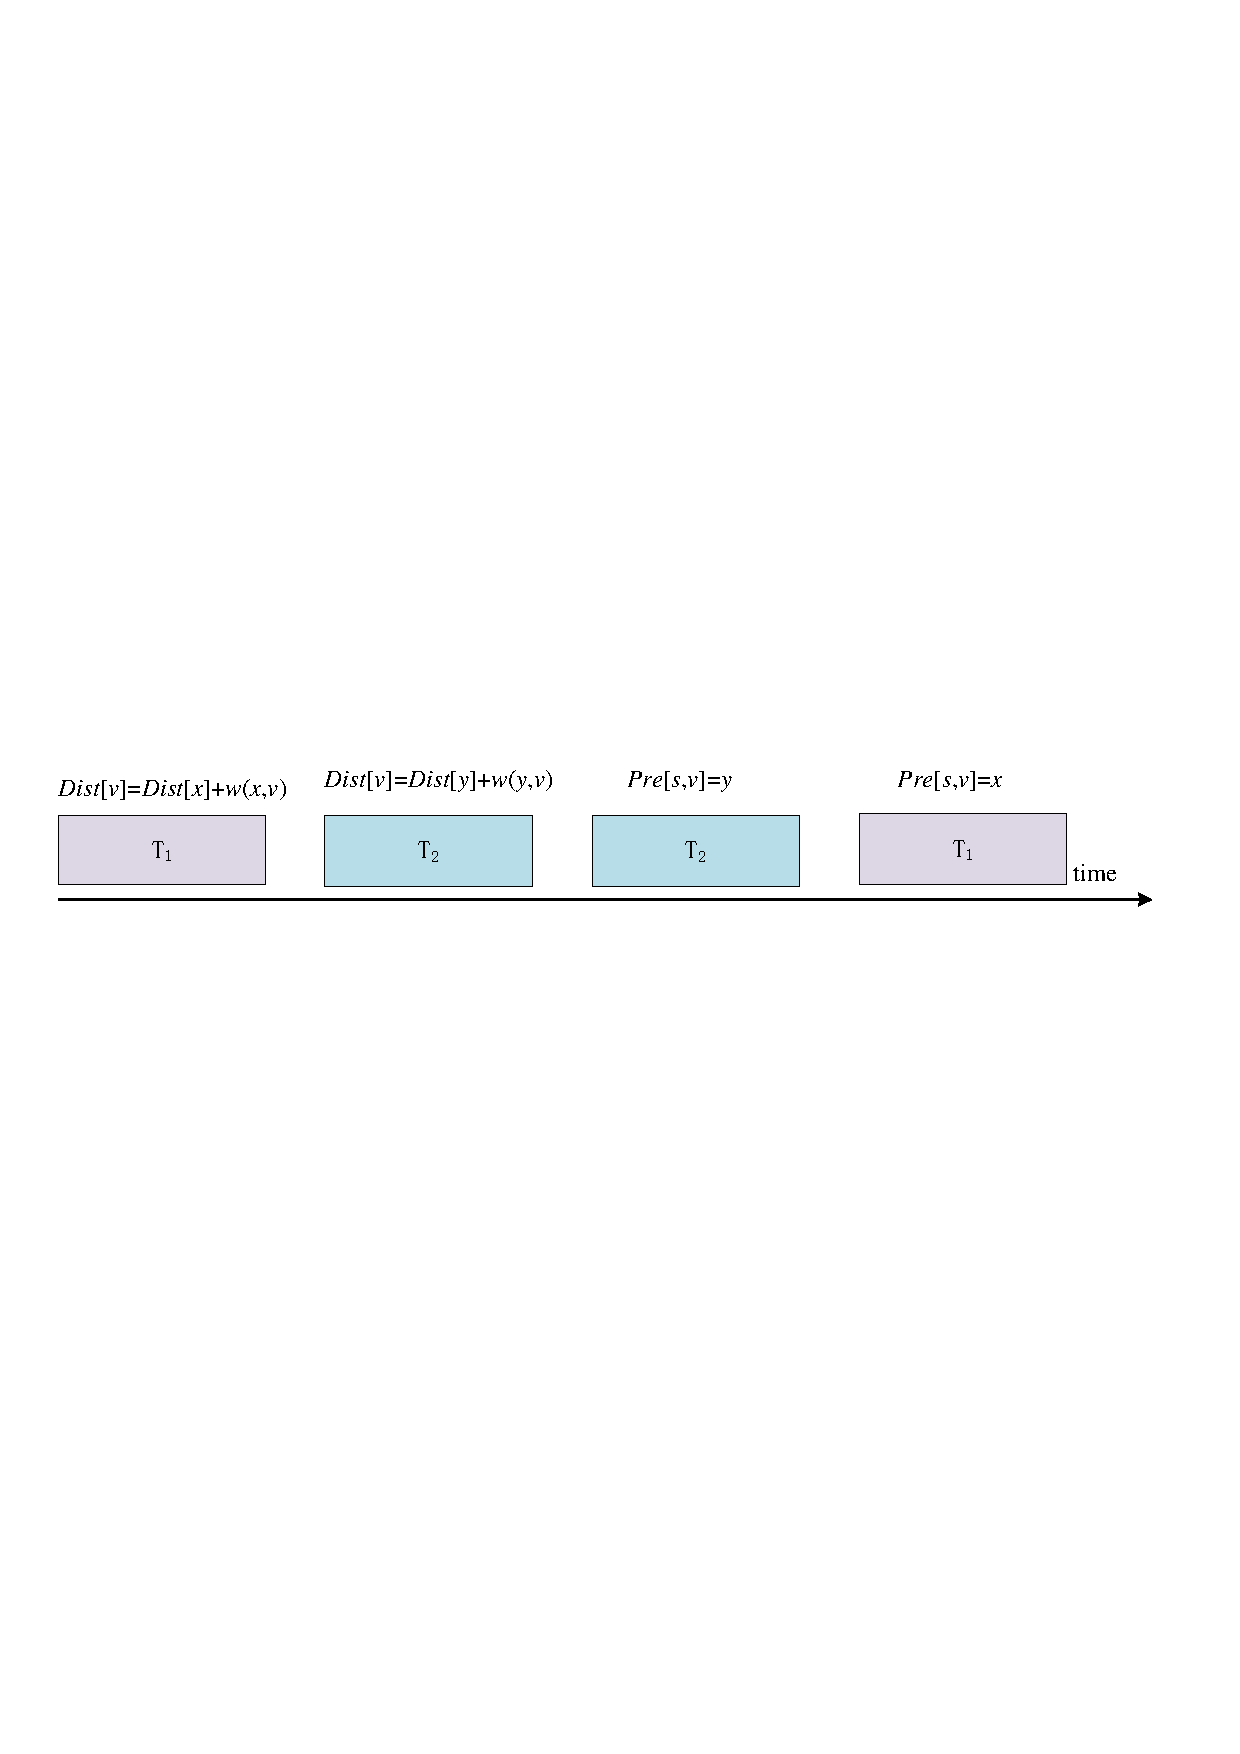
\includegraphics[width=0.8 \textwidth]{figures/SynPro.pdf}}
\end{center}
\caption{{\footnotesize{同步问题的例子}}}
\label{SynPro}
\end{figure*}
最短路径算法CUDA实现算法伪代码如下所示。需要注意的是由于线程在GPU上是独立执行的,在更新节点的距离标记和前驱标记的时候会出现同步问题,假设线程$T_1$为链路$(x,v)$执行松弛操作,而线程$T_2$为链路$(y,v)$ 执行松弛操作,假设两个线程更新点$v$ 的距离标记和更新前驱标记的顺序如图\ref{SynPro} 所示,如果$Dist[y] + w(y, v) < Dist[x] +w(x, v)$,那么$Dist[v]$ 被更新为$Dist[y] + w(y, v)$,但是由于更新的顺序发生交叉,节点$v$的前驱节点被更新成了$x$, 而不是真正正确的前驱节点$y$。为了避免这个同步问题,我们使用两个kernel,一个用来更新距离标号,一个用来更新前驱节点。
\begin{algorithm}[t]
\begin{algorithmic}[1]
\Require
业务需求集合$D$;
链路集合$E$;
\Ensure {业务需求的最短路径结合$P$}
\State {将业务的源节点加入到集合$S$中}
\State {$Mark \leftarrow$ 1}
\While{$Mark > 0$}
\State {$Mark \leftarrow$ 0}
\State {发射 kernel\_distance\_update($S$, $E$, $Dist$)}
\EndWhile
\State {发射 kernel\_predecessor\_update($S$, $E$, $Dist$, $Pre$)}
\State {根据前驱数组$Pre$重建业务的最短路径,并把路径加入到集合$P$中}
\end{algorithmic}
\caption{{并行最短路计算}}
\label{ParaSPC}
\end{algorithm}

\begin{algorithm}[t]
\begin{algorithmic}[1]
\Function{kernel\_distance\_update}{$S$, $E$, $Dist$}
\State {$bid \leftarrow$ block ID}
\State {$tid \leftarrow$ thread ID}
\State {将 $(bid, tid)$ 映射到 id $sid$}
\State {$s \leftarrow S[sid]$}
\State {$e \leftarrow E[bid]$}
\If{$Dist[s][e.tail] + e.weight < Dist[s][e.head]$}
\State {$Mark \leftarrow 1$}
\State {$Dist[s][e.head] \leftarrow Dist[s][e.tail] + e.weight$}
\EndIf
\EndFunction
\end{algorithmic}
\caption{kernel函数 kernel\_distance\_update}
\label{KernelDist}
\end{algorithm}

\begin{algorithm}[t]
\begin{algorithmic}[1]
\Function {kernel\_predecessor\_update}{$S$, $E$, $Dist$,$Pre$}
\State {$bid \leftarrow$ block ID}
\State {$tid \leftarrow$ thread ID}
\State {将 $(bid, tid)$ 映射到 id $sid$}
\State {$s \leftarrow S[sid]$}
\State {$e \leftarrow E[bid]$}
\If{$Dist[s][e.tail] + e.weight = Dist[s][e.head]$}
\State {$Pre[s][e.head]= e.tail$}
\EndIf
\EndFunction
\end{algorithmic}
\caption{kernel函数 kernel\_predecessor\_update}
\label{KernelPre}
\end{algorithm}
\subsection{链路权重更新}
\subsubsection{权重更新步长}
在LR-PROA算法中,在第$(k+1)$次迭代,链路$(i,j)$的权重被更新为$w_{ij}^{k} + \lambda_{ij}^{k+1}$, 其中$\lambda_{ij}^{k+1}$ 被更新为:
\begin{equation}\label{Iter}
\lambda_{ij}^{k+1} = \lambda_{ij}^k + \theta_k[(\sum\limits_{d \in D}x_{ij}^dbw_d - c_{ij})]^+.
\end{equation}
为了保证收敛性,第$k$次迭代的更新步长($\theta_k$)可以被设置为 $\frac{1}{k}$ \citing{NetworkFlow}。 然而,通过仿真发现,当$\theta_k$被设置为 $\frac{1}{k}$时,其收敛缓慢。让我们考虑图 \ref{u1}的例子,其中链路$(i,j)$ 上的标记分别表示链路权重和链路上剩余的容量大小。假设现在有两个业务需求$d_1$ 和$d_2$,他们的源都是$A$,目的节点都是$D$,且每一个业务的流量大小都是4个单位。为了展示这个迭代过程,我们把算法前5次的迭代结果表示在表 \ref{Iterprocess1}中,从表中可以看到,业务计算出的最短路径一直在$A-B-D$和$A-C-D$ 之间徘徊。算法必修等到$A-B-D$ 和$A-C-D$ 的两条路的权重相等时才能停止,只有这样这两个业务才可能分离,其中一个选择$A-B-D$,而另一个选择$A-C-D$。 但是,正如表中所示这需要大量的迭代才能达到。
\begin{figure}
\setlength{\belowcaptionskip}{-0.1cm}
\begin{center}
{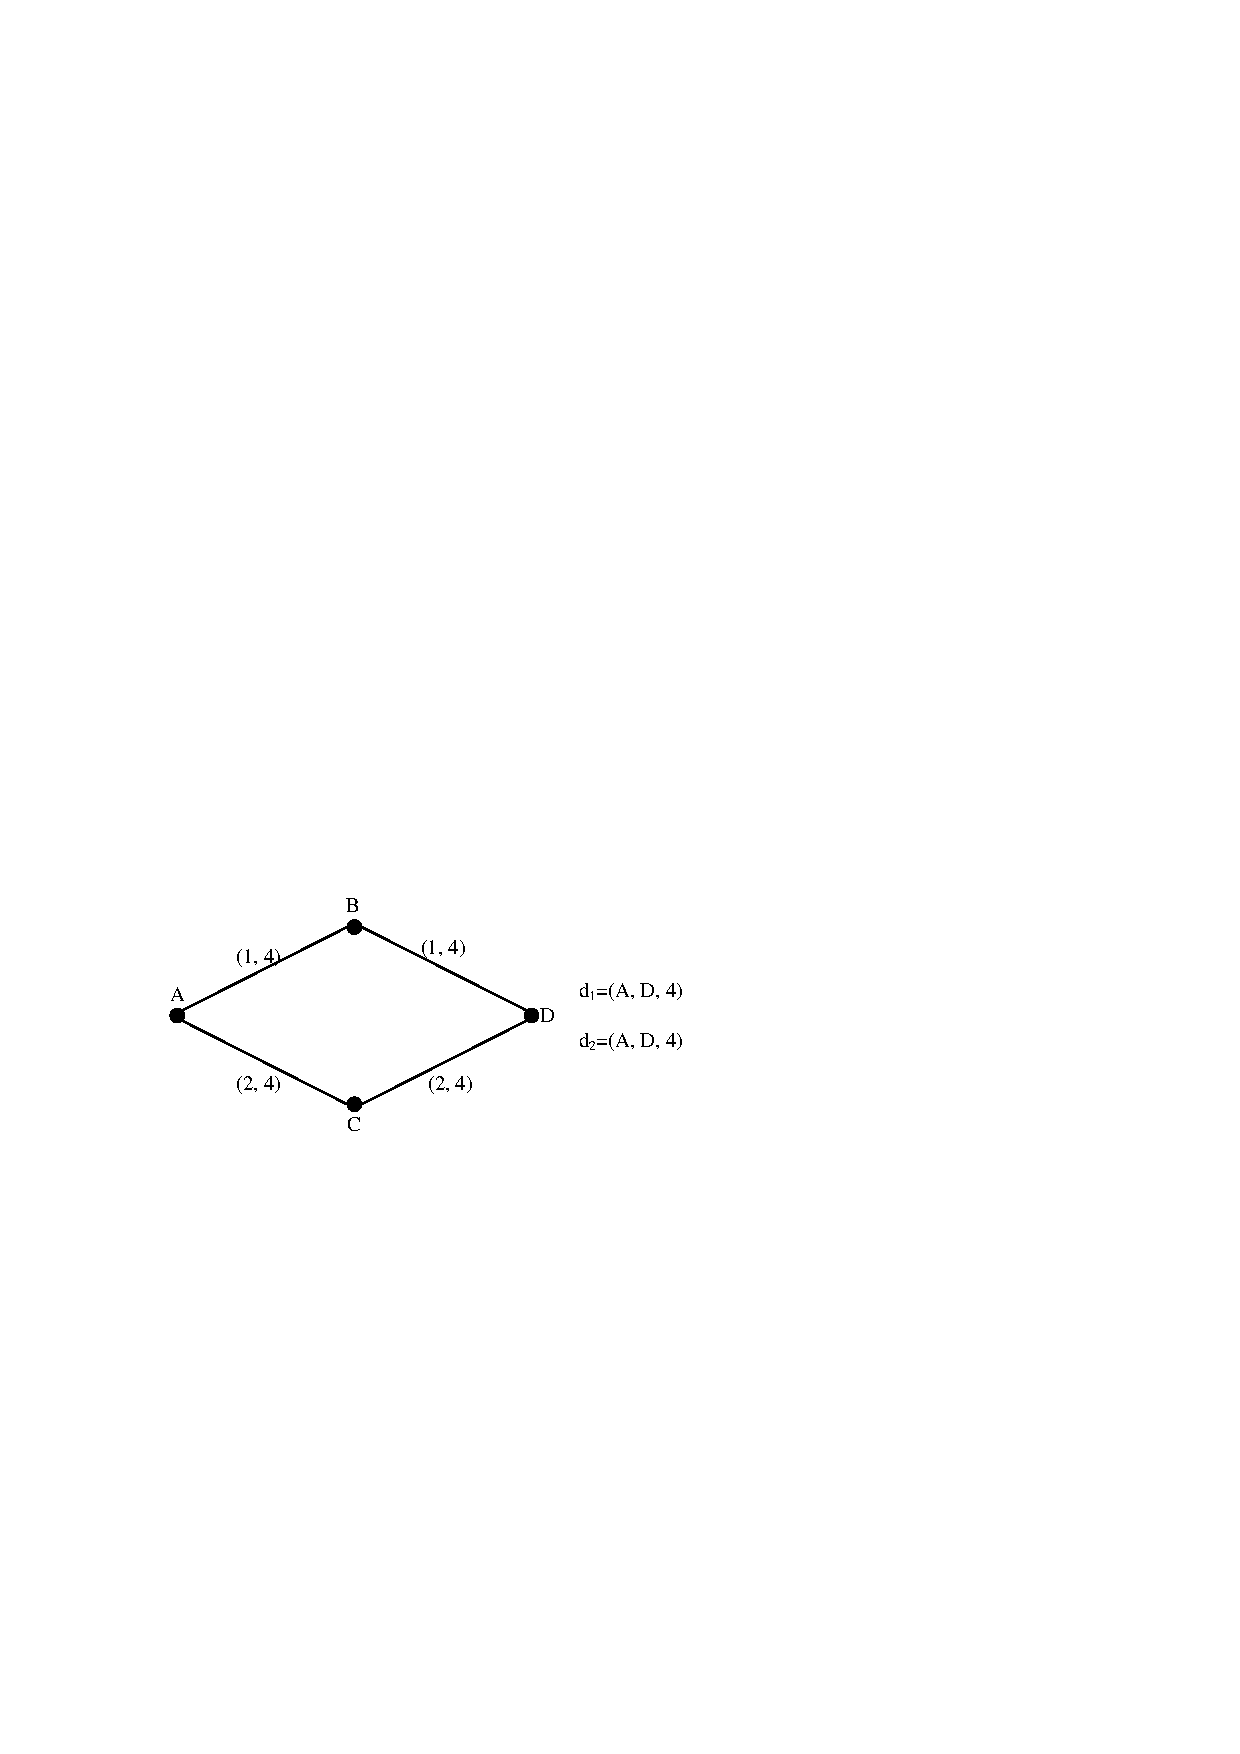
\includegraphics[width=0.4 \textwidth]{figures/IterNum.pdf}}
\end{center}
\caption{{\footnotesize{链路更新例子(1)}}}
\label{u1}
\end{figure}
\begin{table}[t]
\newcommand{\tabincell}[2]{\begin{tabular}{@{}#1@{}}#2\end{tabular}}
\setlength{\abovecaptionskip}{0.2cm}
\centering
\scriptsize{
\renewcommand{\tabcolsep}{0.09cm}
\renewcommand{\arraystretch}{1.2}
\caption{拉格朗日更新过程(1)}
\begin{tabular}{| c | c | c | c|}
\hline
Iteration number & \tabincell{l}{Calculated paths for \\the two demands} & Path weights & $\theta_k$
\\ \hline
0 & \tabincell{l}{A-B-D \\ A-B-D} & \tabincell{l}{2(1+1) \\ 2(1+1)} & 1 \\ \hline
1 & \tabincell{l}{A-C-D \\ A-C-D } & \tabincell{l}{4(2+2) \\ 4(2+2)} & 1 \\ \hline
2 & \tabincell{l}{A-B-D \\ A-B-D} & \tabincell{l}{10(1+4+1+4) \\ 10(1+4+1+4)} & 0.5 \\ \hline
3 & \tabincell{l}{A-C-D\\ A-C-D} & \tabincell{l}{12(2+4+2+4) \\ 12(2+4+2+4)} & 0.33 \\ \hline
4 & \tabincell{l}{A-B-D \\ A-B-D} & \tabincell{l}{14(1+6+1+6) \\ 14(1+6+1+6)} & 0.25 \\ \hline
5 & \tabincell{l}{A-C-D \\ A-C-D} & \tabincell{l}{14.66(2+5.33+2+5.33) \\ 14.66(2+5.33+2+5.33)} & 0.2 \\ \hline
\end{tabular}
\vskip 0.2 cm
\label{Iterprocess1}
}
\end{table}

另外一种常用的步长选择是:
\begin{equation}\label{StepSize}
\theta_k = \frac{\rho[UB-{L(\mathbf{\lambda}^k)]}}{||\mathbf{Ax^k}-\mathbf{b}||^2}
\end{equation}
其中$UB$是最优化目标函数的上界,$\rho$是一个取值范围为0到2的常数,$\mathbf{A}$ 和 $\mathbf{b}$分别是链路相关矩阵和链路上的剩余容量向量。但是从实验中发现设置这种步长迭代效果也不令人满意,因此,本设计采用一种简单但是有效的链路权重更新步长,假设$\theta_{k}^{ij}$ 为第$k$th次迭代时链路$(i,j)$ 上的需更新的步长,那么$\theta_{k}^{ij}$ 为:
\begin{equation}\label{StepSizeUsed}
\theta_{k}^{ij} = \frac{1}{|c_{ij}-\sum\limits_{d \in D} x_{ij}^d bw_d|}
\end{equation}

从式子 \ref{StepSizeUsed},我们可以看到,如果一条链路上承载的流量大小超过了这条链路上的容量大小,那么这条链路上的权重在下一次迭代之前就会增加1, 对于其他的流量满足约束的链路,其权重不会改变,如果使用\ref{StepSizeUsed}的步长更新方法,LR-PROA仅仅只需要一次迭代就能够得到例子中 \ref{u1} 最优的权重,实验表明,这种粗粒度的更新操作大大的减小了算法的收敛迭代次数,从而大大缩短算法运行时间。
\subsubsection{随机更新策略}

拉格朗日松弛法将原问题分解成了一个个独立的最短路径问题,这样使得算法可以并行化进行设计,但是由于每个子问题独立分离,使得每个问题在求最短路径时都是贪心的,这样可能会使得大量业务抢占同一批链路,造成拥塞,一旦拥塞,链路的权重增加,又会使得大量的业务放弃这一批链路,去抢占其他链路,而这些链路由于权重过分增加,造成没有业务去选择他们,使得链路利用出现浪费,甚至会造成其他链路发生拥塞,这样出现恶性循环,最终会使得算法提前收敛到局部最优解,另外,由上一节的分析,为了最求快速收敛,我们简单地将步长设置为$\frac{1}{|c_{ij}-\sum\limits_{d \in D} x_{ij}^d bw_d|}$,就是对把每一个超过容量约束的边简单地增加一,这样粗粒度的增加,可能会加重上面讨论的拥塞循环。
\begin{figure}
\setlength{\belowcaptionskip}{-0.1cm}
\begin{center}
{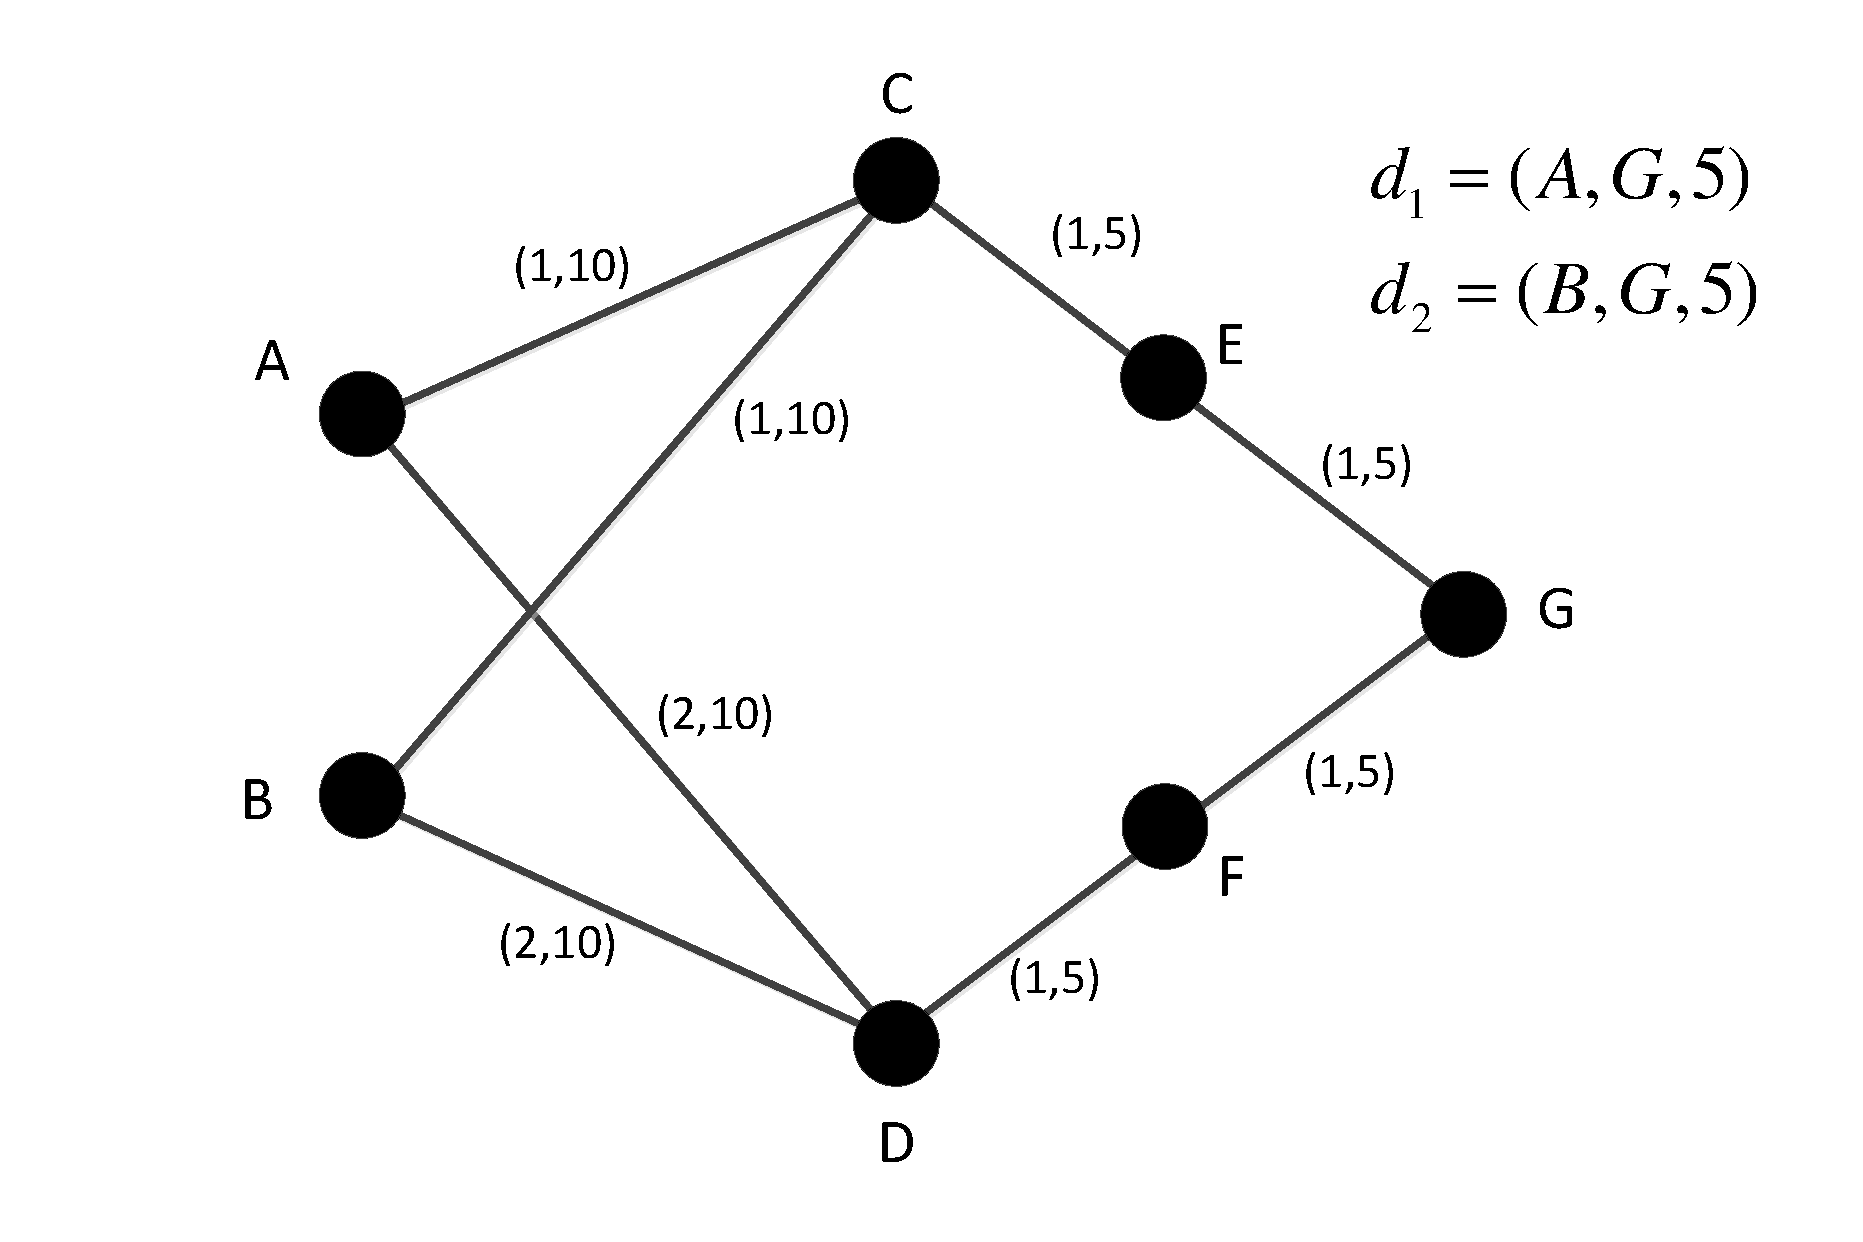
\includegraphics[width=0.4 \textwidth]{figures/random.pdf}}
\end{center}
\caption{{\footnotesize{链路更新例子(2)}}}
\label{u2}
\end{figure}
如图\ref{u2}所示,假设有存在两个业务$d_1$和$d_2$,其中$d_1$的源节点为$A$,目的节点为$G$, 其流量大小为$5$,$d_2$ 的源节点为$B$,目的节点为$G$,其流量大小为$5$,开始时两个都分别贪心计算最短路径,$d_1$ 选择路径$A-C-E-G$,$d_2$选择路径$B-C-E-G$, 这样的话,链路$C-E$和$E-G$出现拥塞,表 \ref{Iterprocess2} 展示了这个迭代过程,图 \ref{u2}中最优的选择是让其中一个业务经过边$C-E-G$进行中继,另一个业务经过边$D-F-G$进行中继。但是的迭代过程始终无法使得两条链路发生分离,图中的链路权重始终无法达到最优条件,这是因为算法的权重迭代增加粒度太大,由于链路$C-E-G$和链路$D-F-G$每次超限都会为路径的总权重增加2个单位,假设每次迭代时链路$C-E-G$和链路$D-F-G$ 每次迭代时一共只贡献1个单位的权重增加,那么算法只需要一次迭代就能达到最优条件,此时链路$C-E-G$由于超限,权重一共增加1个单位,那么路径$A-C-E-G$ 和路径$A-D-F-G$ 权重相等都为4,同样,路径$B-C-E-G$和路径$B-D-F-G$的权重也相等了,这样两个业务才会分离开(比如业务$d_1$选择链路$A-C-E-G$, 业务$d_2$选择链路$B-D-F-G$)。但是在算法设计时,我们难以分辨哪些链路的组合会引起业务出现这种徘徊情况,为了解决链路增加粒度过大的情况,在本设计中我们采用随机选择执行更新的策略,也就是对一条流量超过容量约束的边$(i,j)$,我们以概率$\phi$ 来对他进行权重更新,每条边的权重增加粒度依然为1个单位,假设$\phi=0.5$,这种方法在一定概率上保证图 \ref{u2} 中的例子可以在一次迭代中收敛。实际实验中发现这种更新策略能够保证算法得到较优解的同时,保证收敛速度较快。
\begin{table}[t]
\newcommand{\tabincell}[2]{\begin{tabular}{@{}#1@{}}#2\end{tabular}}
\setlength{\abovecaptionskip}{0.2cm}
\centering
\scriptsize{
\renewcommand{\tabcolsep}{0.09cm}
\renewcommand{\arraystretch}{1.2}
\caption{拉格朗日更新过程(2)}
\begin{tabular}{| c | c | c |}
\hline
Iteration number & \tabincell{l}{Calculated paths for \\the two demands} & Path weights
\\ \hline
0 & \tabincell{l}{A-C-E-G \\ B-C-E-G} & \tabincell{l}{3(1+1+1) \\ 3(1+1+1)} \\ \hline
1 & \tabincell{l}{A-D-F-G \\ B-D-F-G } & \tabincell{l}{3(2+1+1) \\ 3(2+1+1)} \\ \hline
2 & \tabincell{l}{A-C-E-G \\ B-C-E-G} & \tabincell{l}{3(1+2+2) \\ 3(1+2+2)} \\ \hline
3 & \tabincell{l}{A-D-F-G\\ B-D-F-G} & \tabincell{l}{3(2+2+2) \\ 3(2+2+2)} \\ \hline
4 & \tabincell{l}{A-C-E-G \\ B-C-E-G} & \tabincell{l}{3(1+3+3) \\ 3(1+3+3)} \\ \hline
5 & \tabincell{l}{A-D-F-G \\ B-D-F-G} & \tabincell{l}{3(2+3+3) \\ 3(2+3+3)}\\ \hline
6 & \tabincell{l}{ ...\\ ...} & \tabincell{l}{... \\ ...}\\ \hline
\end{tabular}
\vskip 0.2 cm
\label{Iterprocess2}
}
\end{table}
\subsection{路径调整}
注意到,在最优的权重代价(最优拉格朗日乘子)下,LR-PROA求解到的路径集合解是拉格朗日对偶问题的优化解,但是它不一定是原来路由优化问题的可行解。作为一个例子,考察图 \ref{ppt}中的情况,图中的元组中数字分别表示链路的代价和链路上的剩余容量大小,我们假设有两个业务需求$d_1$和$d_2$,其中两个业务的流量需求都是1个单位,假设在某一个迭代过程中,LR-PROA为两个业务算出来的链路都是$A-C-E-D$, 这条路径选择是对偶问题的最优解,但是他不是原问题的可行解,因为链路$(C,E)$ 上承载的链路容量大于了链路$(C,E)$ 上的容量。这是由于每个业务在选择路径的时候没有去考虑其他业务所选择的路径,但是我们容易看到这个例子中所有路径权重都一样(都等于3),也就是说,图中存在着大量的等价链路,但是在这个例子中两个业务恰好都选择了冲突的那一条路径$A-C-E-D$,如果业务$d_1$的路径被调整到$A-D$,业务$d_2$的链路被调整到$B-F$,那么,我们可以得到原问题的最优可行解,所以通过这里的启发,我们发现需要设计一种业务路径调整算法来主动避免链路出现冲突,来得到原问题的优化的可行解。
\begin{figure}
\setlength{\belowcaptionskip}{-0.1cm}
\begin{center}
{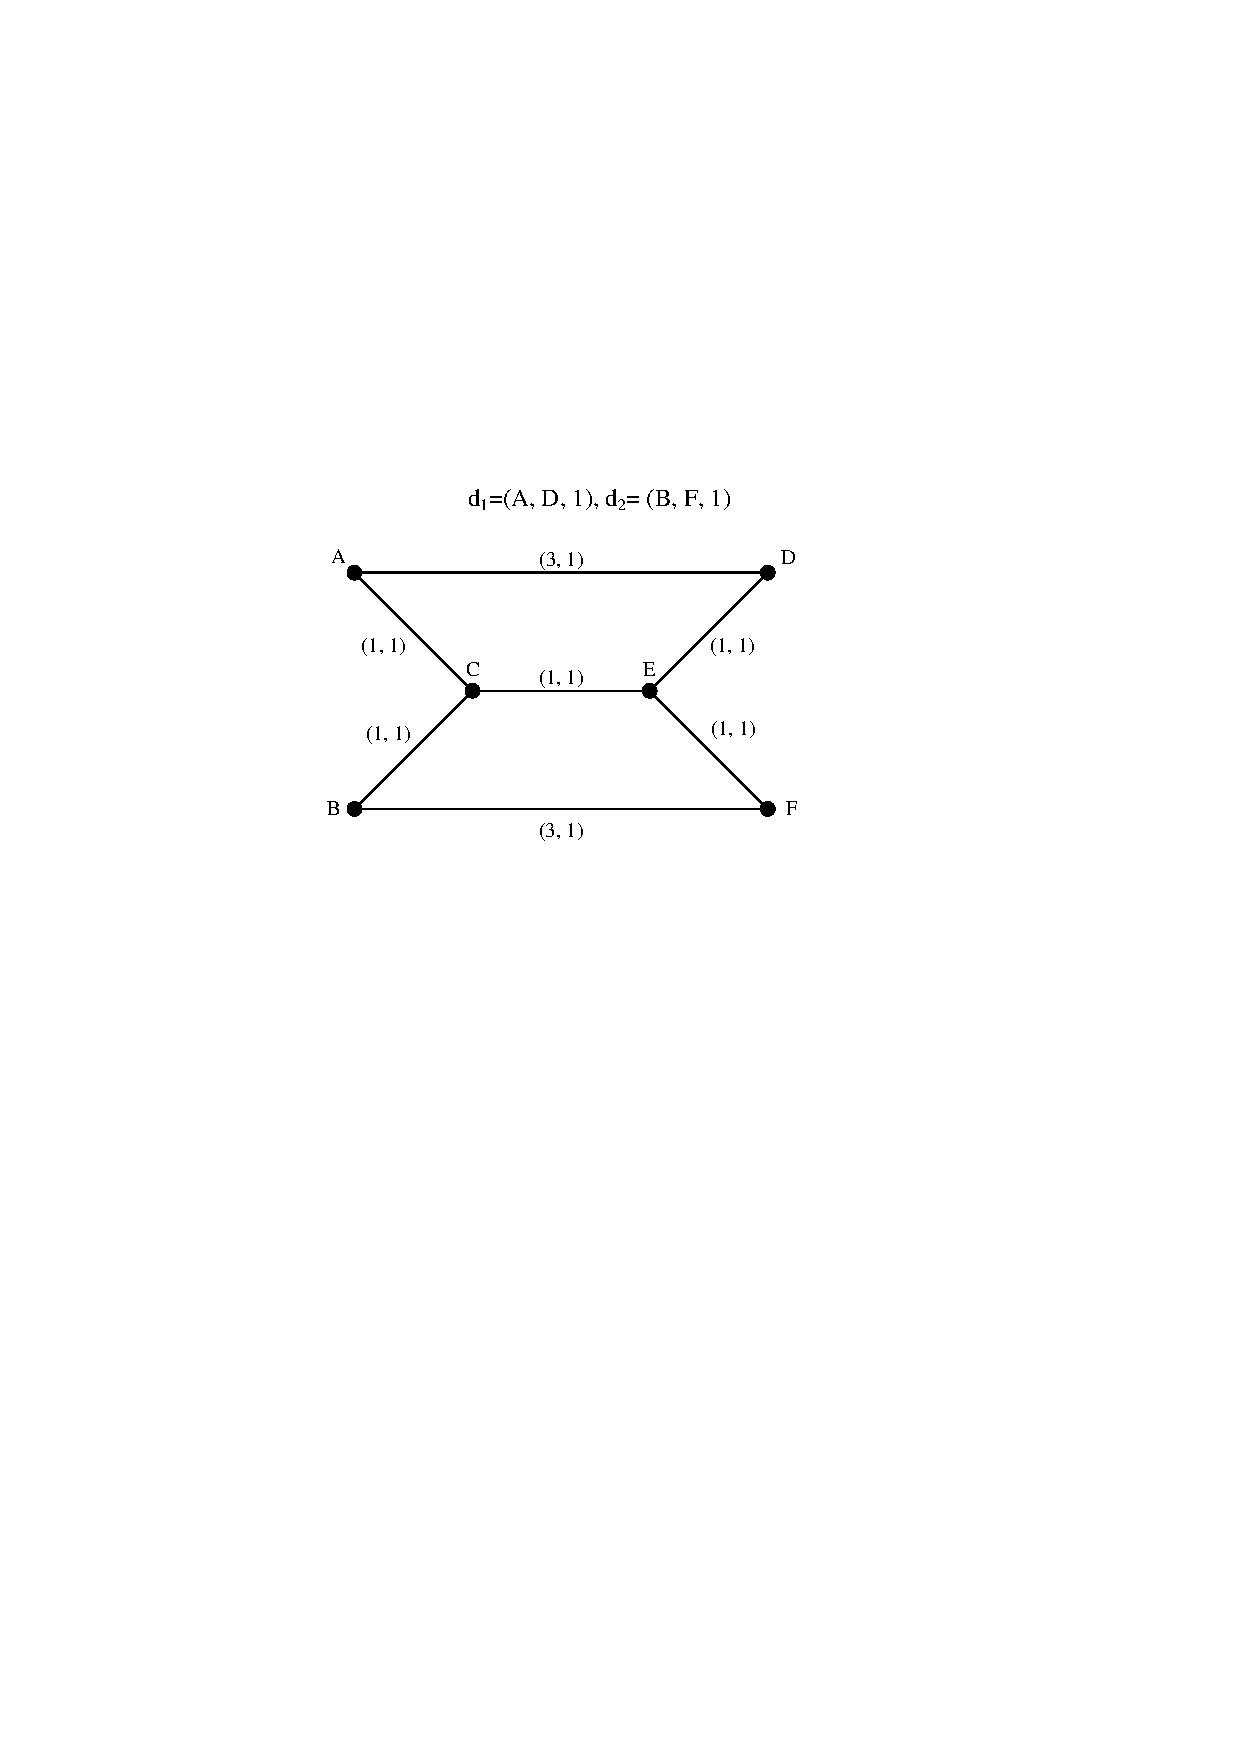
\includegraphics[width=0.4 \textwidth]{figures/PathAdj.pdf}}
\end{center}
\caption{{\footnotesize{路径调整例子}}}
\label{ppt}
\end{figure}
为了说明业务路径调整算法,我们引入一些符号,假设$P$表示步骤2所计算出来的路径集合,其中$p_d\in P$ 表示业务$d$ 的路径, $rp_{d}$ 表示路径$p_d$上的可用带宽,$rp_{d} = min\{r_e | e\in p_d\}$,其中$r_e$ 表示链路$e$上的剩余带宽,$D_l$ 表示剩余业务集合,表示这些业务不能在不违背容量约束的情况下被加入网络中。
\begin{algorithm}[t]
\begin{algorithmic}[1]
\Require
网络拓扑 $G(V, E)$;
业务量需求集合 $D$;
步骤2算出来的路径集合 $P_{in}$;
\Ensure
调整后的路径集合 $AP$;
\State {把业务按照值$\frac{bw_d}{\sqrt{|p_d|}}$进行降序排序}
\For{each traffic demand $d \in D$}
\If{$rp_{d} \ge bw_d$ }
\State{把路径 $p_d$加入到$AP$中}
\State{在图G(V,E)中更新路径$p_d$所经过链路的剩余带宽}
\Else
\State {把业务$d$加入到剩余集合$D_l$中}
\EndIf
\EndFor
\State{$G^{'}(V^{'},E^{'})=G(V,E)$}
\For{each traffic demand $d \in D_l$}
\State{$G^{''}(V^{''},E^{''})=G^{'}(V^{'},E^{'}$}
\For{each link $e \in E^{'}$}
\If{链路$e的剩余容量< bw_d$}
\State{把链路 $e$ 从图$G^{''}(V^{''},E^{''})$中移除}
\EndIf
\EndFor
\State{在图$G^{''}(V^{''},E^{''})$中为业务$d$计算最短路径$p$(链路代价都设为1)}
\If{$\frac{|p|}{|p_d|}\le \delta$}
\State{把路径 $p$ 加入到 $AP$,并把业务从集合$D_l$中移除}
\State{在图$G^{'}(V^{'},E^{'})$中更新路径$p$所经过链路的剩余带宽}
\State{$G(V, E)=G^{'}(V^{'},E^{'})$}
\EndIf
\EndFor
\end{algorithmic}
\caption{路径调整算法}
\label{PathAdj}
\end{algorithm}

路径调整算法的主要思想是通过调整一小部分业务的路径来得到原问题的优化可行解,算法首先对业务进行排序,这里采用3.3.1.2类似的思想对业务进行排序,一方面,要使得目标函数变小,那些流量需求较大的业务应该优先被加入到网络中,但是如果大流量的业务的路由代价很大,经过了一条很长的路径,就会大量的浪费网络中的链路容量资源,所以算法过程对当前解中的业务和其路径按照$\frac{bw_d}{\sqrt{|p_d|}}$的值进行排序,其中${bw_d}$代表业务$d$所需要的流量大小,$|p_d|$代表业务$d$的路径$p_d$的代价大小,这样按照顺序试图将业务加入到网络中,如果$rp_d>=bw_d$,表示业务可以被加入到网络中,那么加入此业务并且更新网络链路的剩余容量值,反之,如果$rp_d<bw_d$,则表示业务选择的路径上的链路容量不足以承载此业务,那么将业务加入剩余集合$D_l$ 中,循环结束后,得到一个剩余网络。根据前面的讨论,在剩余网络中可能存在一些等价路径,剩余链路中依然有很多可用资源,所以算法重新在剩余网络中为剩余业务计算路径,算法依次遍历集合$D_l$,看能否在剩余网络中为业务寻找一条路径,首先剔除那些链路剩余容量小于业务流量$bw_d$ 的链路,这样保证求出来的路径肯定是满足容量约束的,由于剩余链路是残余网络,所以可能会求出跳数很长的路径,如果跳数太长了,会占用太多的资源,不能达到优化的目的,所以我们对跳数进行约束,如果$|p|/|p_d|<\delta$,则将业务加入到网络中,并更新网络链路容量,否则不加人业务到网络中。虽然这个过程是串行的,但是这个过程是很快速的,这主要有以下原因:第一,由于剩余网络中的链路容量普遍较小,能参与计算的链路很少,对一个剩余业务$d$,在计算路径之前,算法会剔除那些剩余容量小于$bw_d$的链路,所以实际上参与计算的网络拓扑很小。第二,剩余业务量集合$D_l$本身较小,算法越往后面加入业务,可用链路会越来越小,网络会进一步变小。通过这个路径调整算法,可以得到原问题的一个优化可行解,这个解作为当前迭代产生的最优解,和全局最优解进行比较,如果这个解优于全局最优解则更新全局最优解。
\subsection{仿真实验分析}
\subsubsection {仿真介绍}

为了证明LR-PROA和GA-PROA的优化效果,我们把两个算法的优化结果和基于备选路径的MILP模型\citing{multi-commodity}的最优目标值进行比较,其中每个业务的备选路径数量为30条,我们使用CPLEX \citing{CPLEX}来求解MILP模型,由于CPLEX求解MILP需要很大的计算量,对于大规模的网络,我们无法得到MILP的最优值,因此我们设置了10分钟的求解时间限制,当Cplex求解时间超过10分钟后,我们停止求解过程,记录求得Cplex 求解的最优可行目标函数,以及MILP模型的最优值得下界。
为了观察LR-PROA和GA-PROA的加速效果,我们分别设计两个算法串行版本LR-PROA和GA-PROA,并把LR-PROA和GA-PROA 与LR-PROA 和GA-PROA进行比较,其中LR-PROA中的路由算法采用带堆优化的dijkstra 算法,dijkstra算法的复杂度为($|N|\lg |N| +|E|$), 为了体现LR-PROA的加速效果,本文还对串行的dijkstra进行了进一步的优化,讨论如下:假设一批业务$D$ 的源节点相同,这一批业务的目的节点组成集合$D$,那么我们在求解dijkstra 算法时,当最小堆吐出了$D$ 中的所有点之后,我们就提前结束了dijkstra,所以当集合$D$ 比较小时,实际的算法复杂度一般是小于($|N|\lg |N| +|E|$) 的。

我们分别采用ERdos-Renyi (ER) \citing{ER}和 Barab asi-Albert (BA) \citing{BA}两种模型来生成实验网络拓扑,实验中的网络拓扑中点的平均度数为6。 我们分别比较算法的目标函数,加速效果和算法的收敛性质,LR-PROA和LR-SROA中的$\delta$和$K$被分别设置为10 和30。GA-PROA与LR-PROA 都是通过CUDA 8.0 进行设计,跑算法的服务器配置有四个Intel Xeon E5-2630 CPU 和一个 NVIDIA Tesla K40M GPU。
\subsubsection{目标函数比较}
图 \ref{OB-TA-200}和图 \ref{OB-TA}分别显示了在点数为200和1000的网络中,目标函数随着业务数量规模变化的折线图,图中的网络链路容量大小为100,业务的流量需求大小为$[1,100]$的均匀随机值。从图中我们可以看到目标函数大致随着业务数量呈现线性增加,这和目标函数的表达式相吻合。从图中可以看到LR-SROA/LR-PORA的算法优化目标明显优于遗传算法LR-PROA/LR-SROA,这是因为:1. 遗传算法提前陷入了局部最优解,导致算法提前结束。2.遗传算法是基于备选路径的,所以其没有LR-SPOA/LR-PROA 那么灵活, LR-SPOA/LR-PROA 会动态的寻找业务的路径,根据网络链路的动态状况重新求解路径,从而充分利用网络链路资源,从而减小目标函数。

和MILP的Cplex解相比,在小网络(点为200)中,由于Cplex的计算压力不大,其计算出来的解略微优于LR-SPOA/LR-PROA。
可以看到图中MILP-bound和LR-SPOA/LR-PROA差距很小,这说明在小网络下,LR-SPOA/LR-PROA 算法求出的解已经很接近MILP 的理论最优解了;在大网络中,由于Cplex的计算压力增大,LR-SPOA/LR-PROA的解已经优于Cplex 的解。比较MILP-bound 我们可以发现LR-SPOA/LR-PROA的解离MILP-bound 有一定差距,这是可能有两个原因:1.Cplex的计算压力大,导致求得的bound可能不够精确。2.LR-SPOA/LR-PROA陷入了局部最优解。
图 \ref{OB-CA-200}和图 \ref{OB-CA}表示在容量变化下的目标函数值变化,其中业务数量为点数的6倍,网络链路容量从100到250变化。随着容量的增加目标函数大致呈现线性下降,这是因为链路容量增加后,网络资源增大,网络可容纳的业务增加,业务可选择的优化路径增增多,业务的路径代价下降,阻塞的大量减少,所以目标函数呈现大幅下降。
\begin{figure}
\setlength{\belowcaptionskip}{-0.1cm}
\begin{center}
{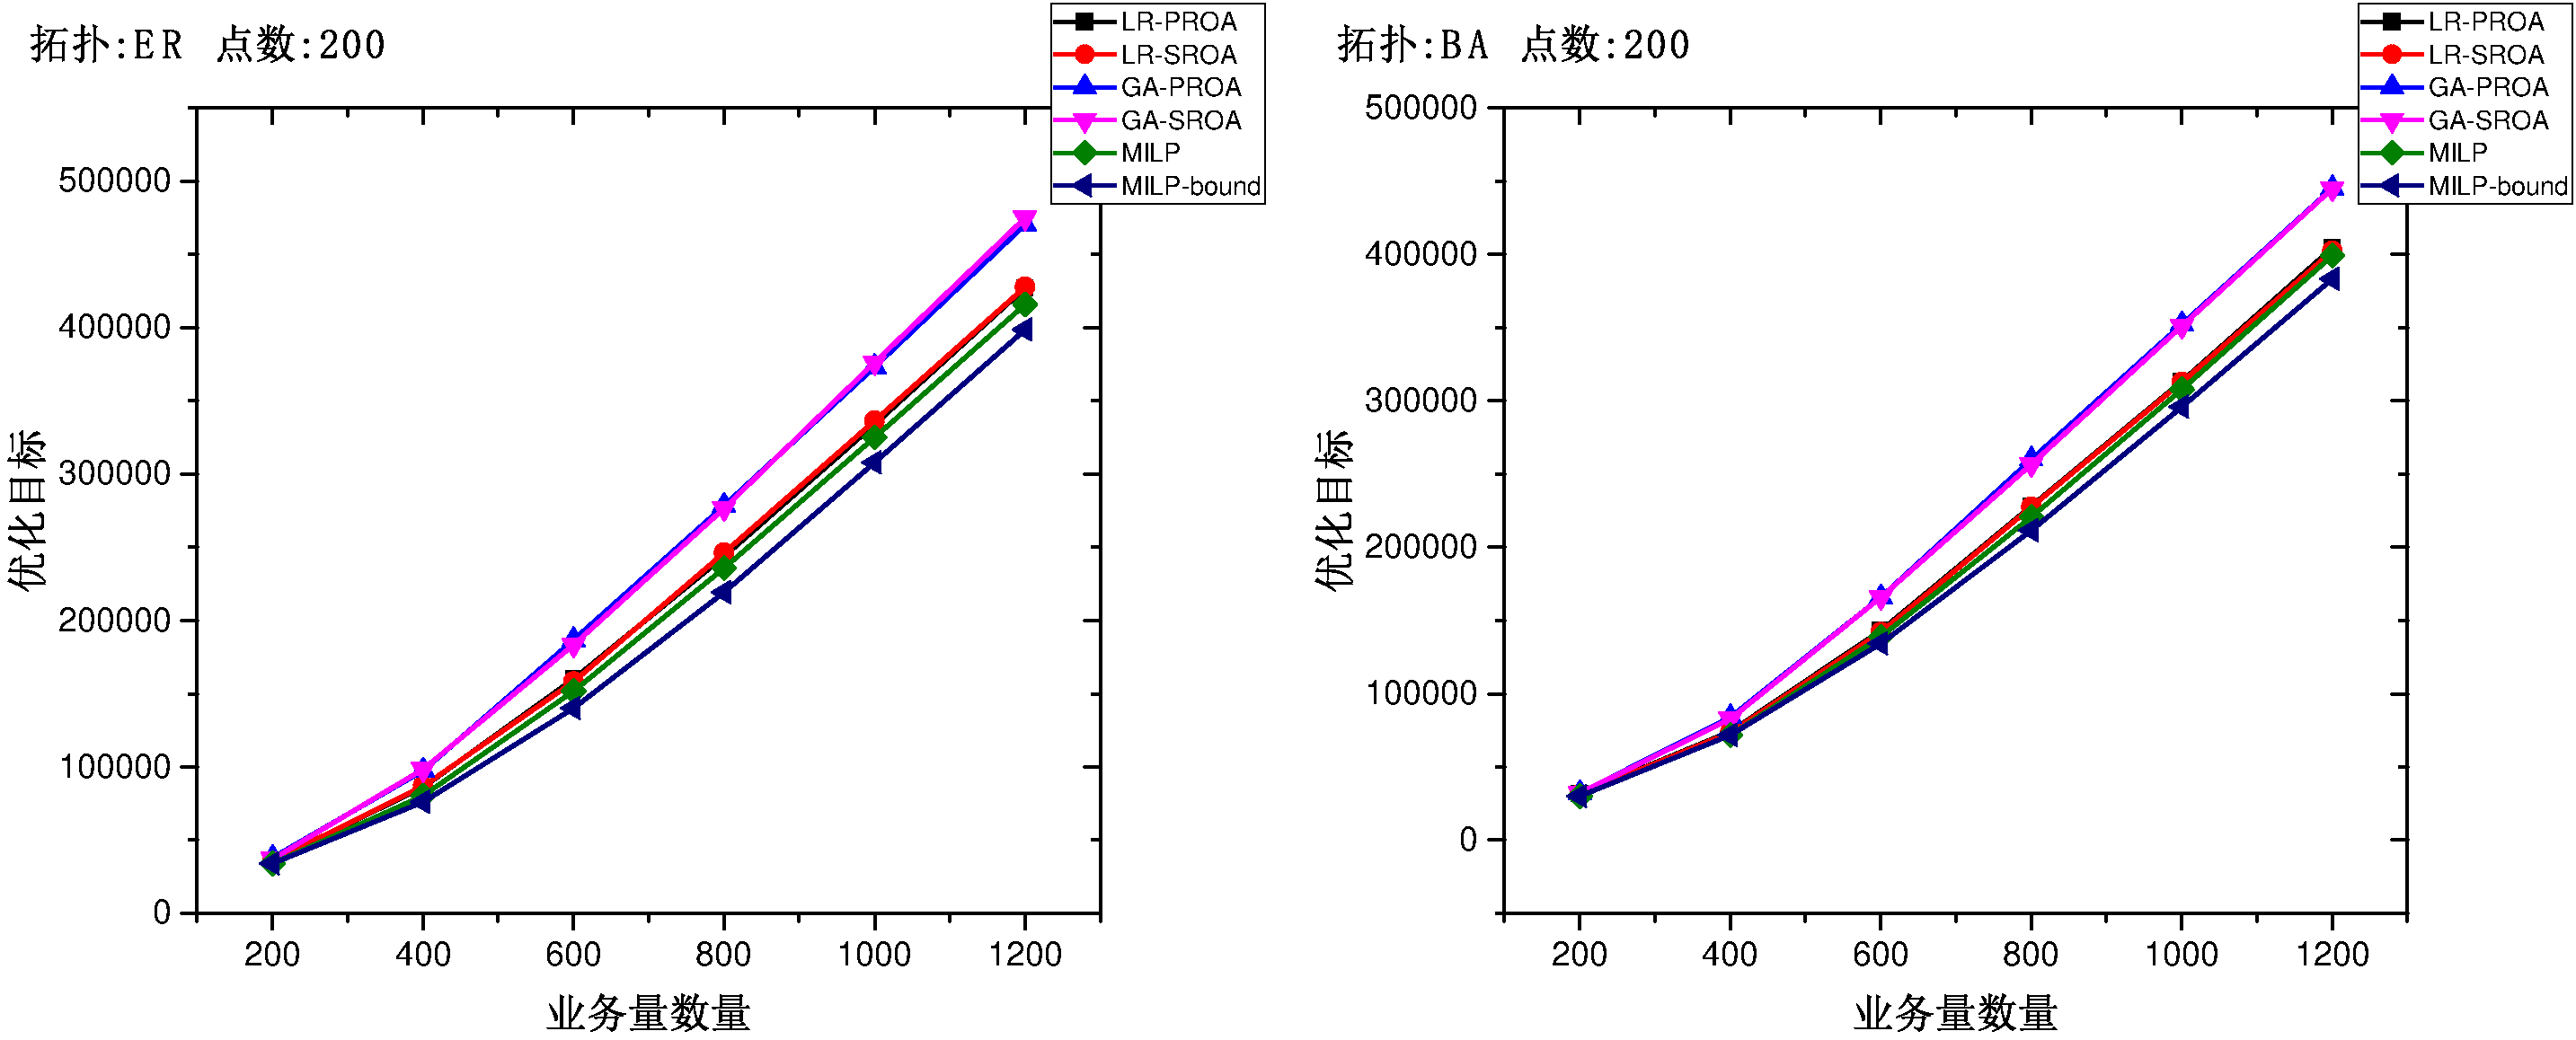
\includegraphics[width=0.8 \textwidth]{figures/OB-TA-200.pdf}}
\end{center}
\caption{{\footnotesize{Object-Task(200)}}}
\label{OB-TA-200}
\end{figure}
\begin{figure}
\setlength{\belowcaptionskip}{-0.1cm}
\begin{center}
{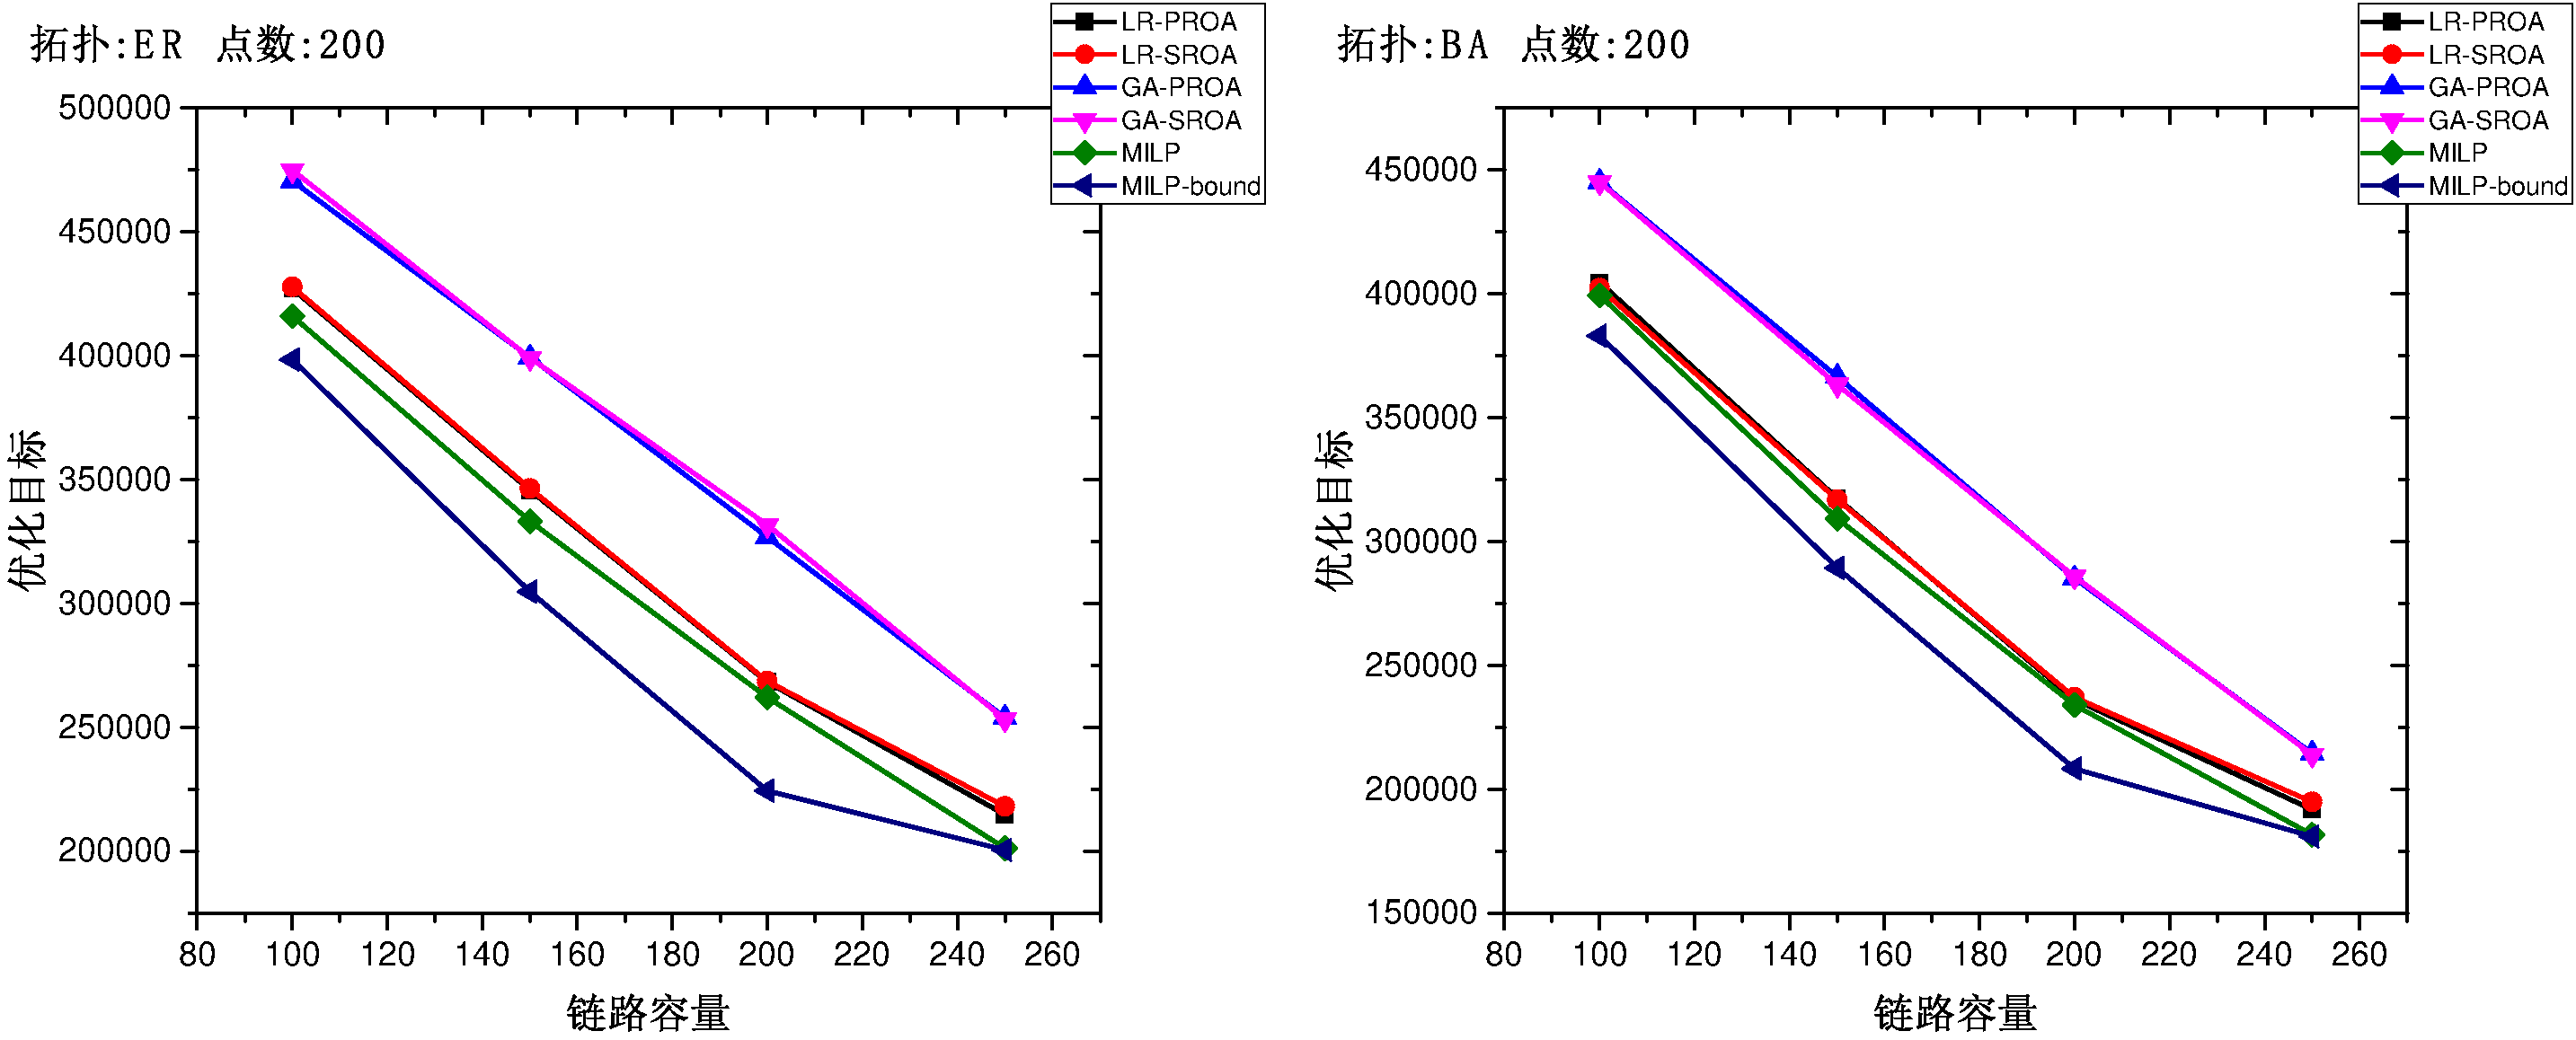
\includegraphics[width=0.8 \textwidth]{figures/OB-CA-200.pdf}}
\end{center}
\caption{{\footnotesize{Object-Capacity(200)}}}
\label{OB-CA-200}
\end{figure}
\begin{figure}
\setlength{\belowcaptionskip}{-0.1cm}
\begin{center}
{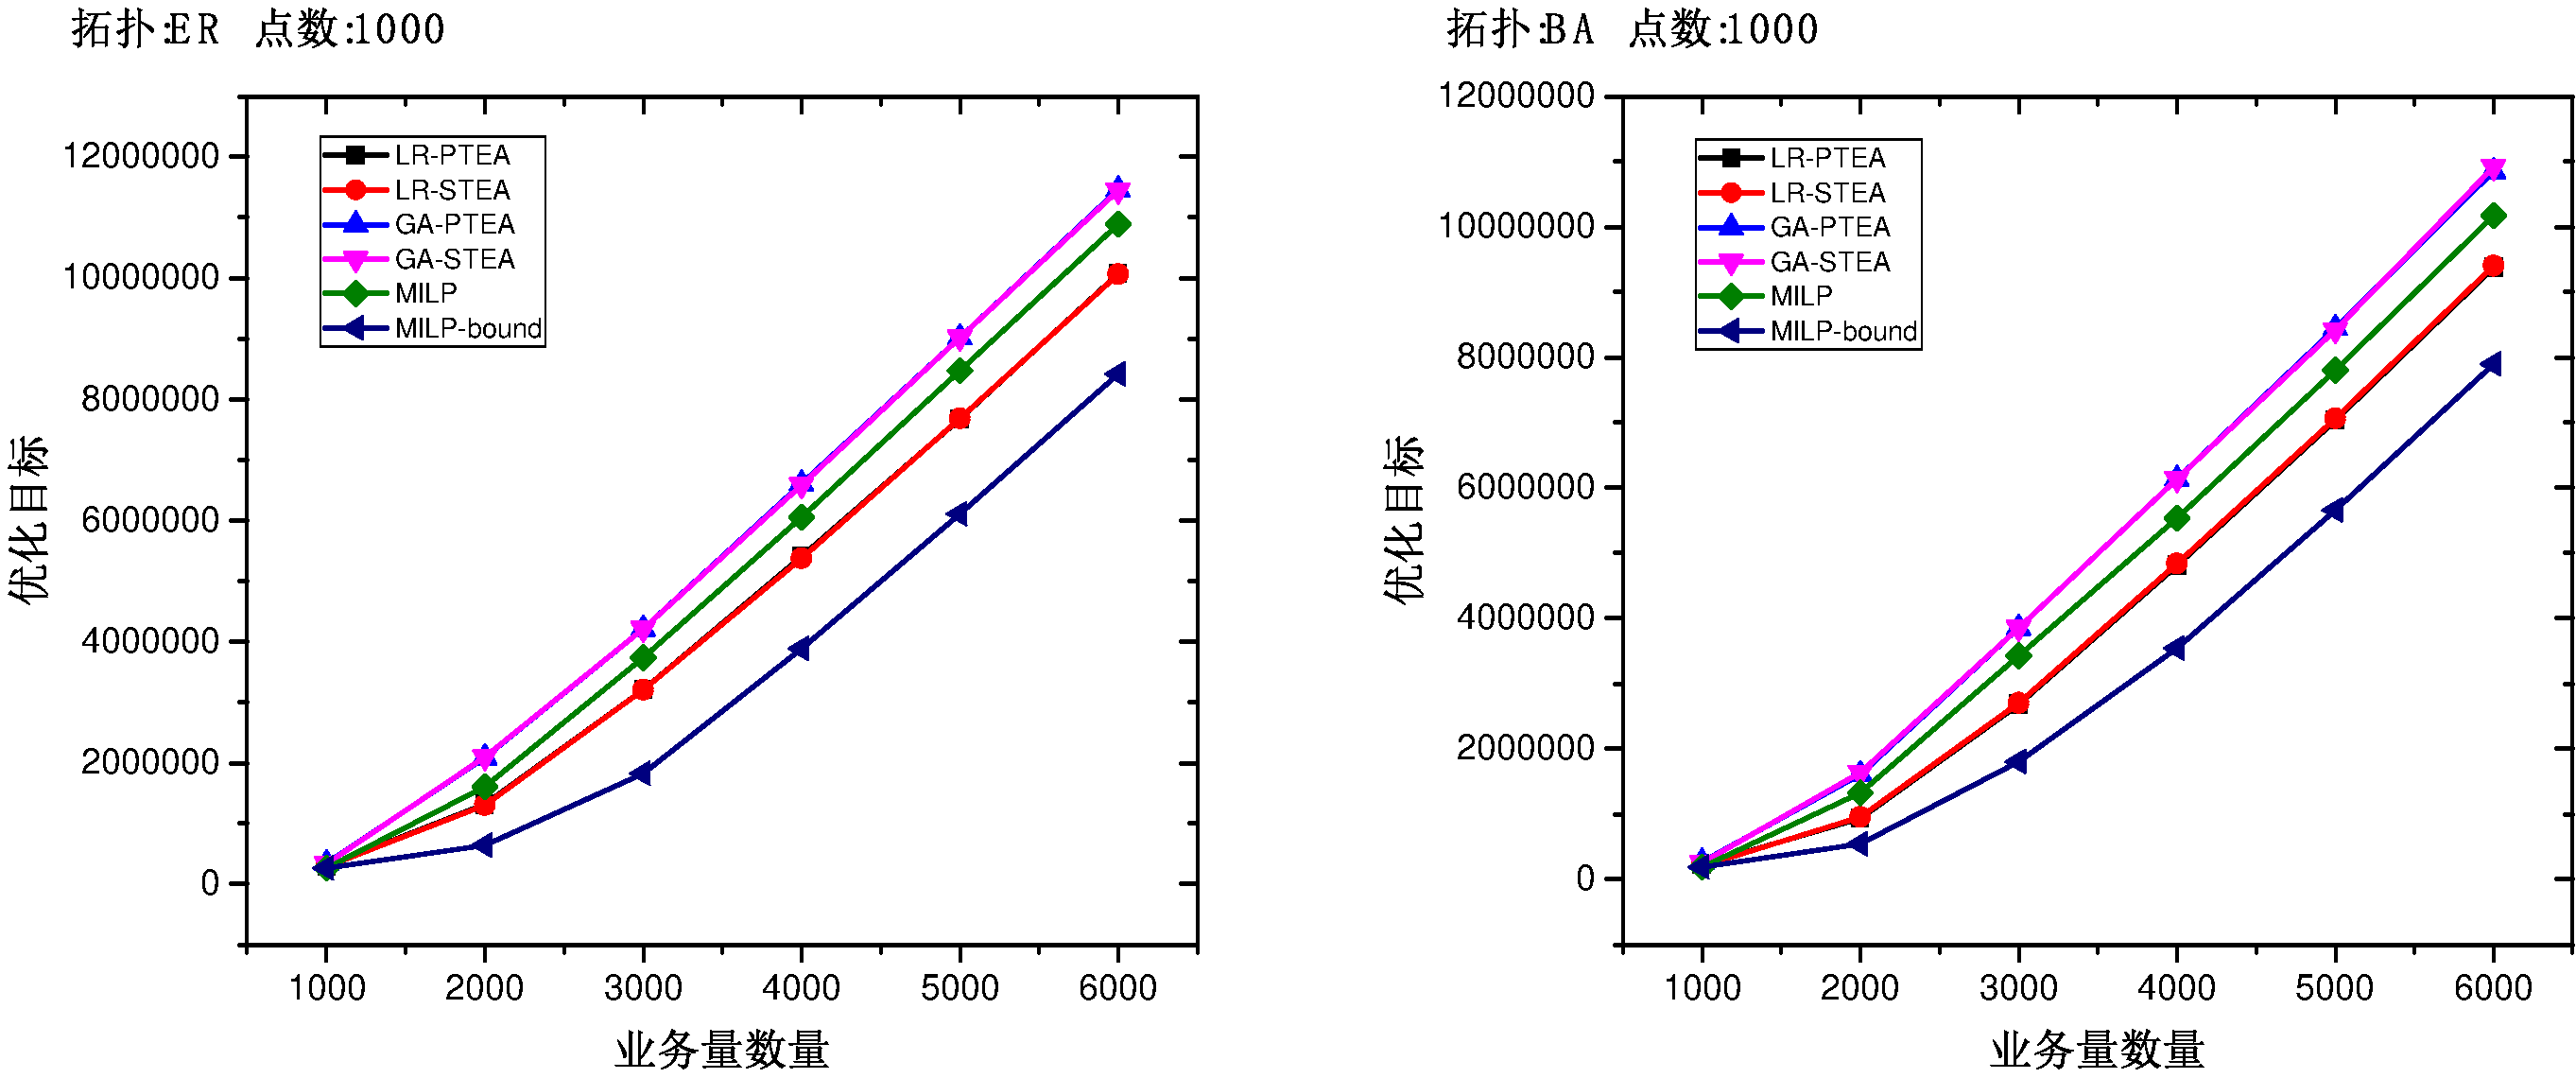
\includegraphics[width=0.8 \textwidth]{figures/OB-TA.pdf}}
\end{center}
\caption{{\footnotesize{Object-Task(1000)}}}
\label{OB-TA}
\end{figure}
\begin{figure}
\setlength{\belowcaptionskip}{-0.1cm}
\begin{center}
{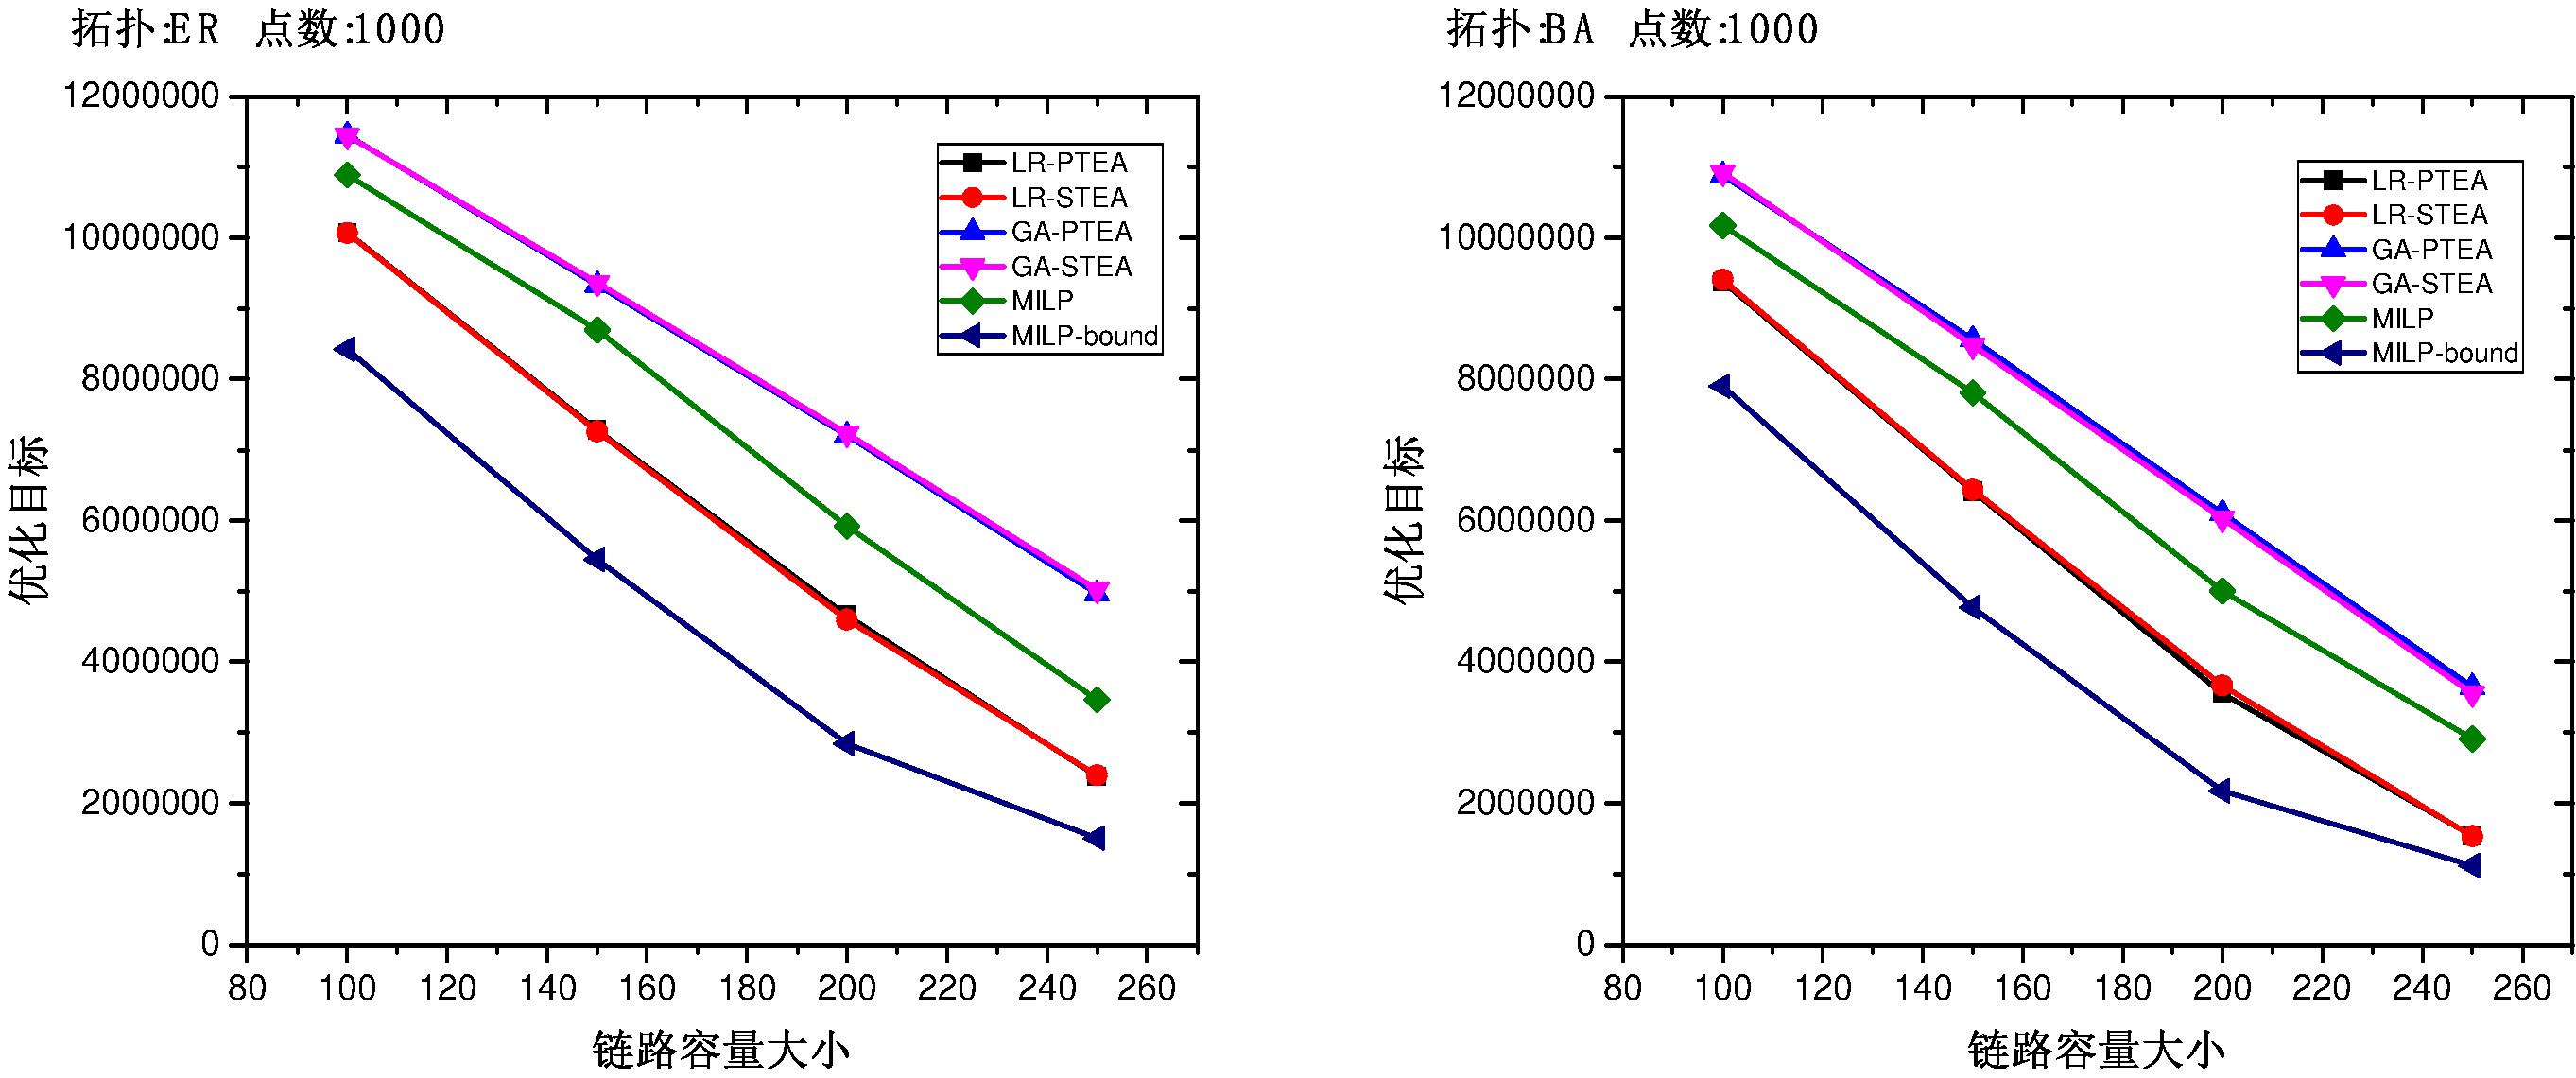
\includegraphics[width=0.8 \textwidth]{figures/OB-CA.pdf}}
\end{center}
\caption{{\footnotesize{Object-Capacity(1000)}}}
\label{OB-CA}
\end{figure}
\subsubsection{算法时间比较}
图 \ref{TI-ER-TA-1000}和图 \ref{TI-BA-TA-1000}分别列出了算法在BA和ER拓扑下的计算时间随着业务数量增加的变化情况,图中拓扑节点数量为1000,业务数量从1000 到6000变化,业务流量为1到100的均匀随机值,链路的容量为100。由于各种算法的时间差距过大,我们用三种不同的尺度进行展示。首先,CPlex的时间限制都为10分钟,所以我们不再列出来。

图中我们可以看到GA-PROA相对于GA-SROA加速很多大约为30倍左右,但是由于遗传算法本身的缺陷,所以GA-PROA的计算时间是很糟糕的,这是因为基于备选路径的遗传算法的初始值染色体较差,所以需要大量的迭代次数才能收敛,而且遗传算法评价步骤的本身的计算量也很大。

观察LR-SPOA和LR-PROA,发现LR-SPOA和LR-PROA的时间曲线会发生大幅度的波动,这是因为,算法的迭代次数变化较大,我们设置算法在30次后未找到更优解之后停止,其实30次设置得偏小,算法有可能会找到更好的解,但是这些解的优化程度很小(通过收敛图 \ref{CO-LR-1000},可以看到算法在前50次内下降幅度较大,后面的下降幅度很小),所以为了优化整体时间,我们设置迭代次数为较小的30 次,由于30 偏小,所以可能会导致算法的提前结束,从而导致算法的迭代次数变化幅度较大,从而引起整体时间上的幅度变化。

观察图 \ref{TI-ER-TA-1000}和图 \ref{TI-BA-TA-1000},我们发现当业务数量增加到两倍点数以上后,LR-PROA相对于LR-SROA有较大加速,其中拓扑大小为1000 时,LR-PROA 相对与LR-SROA有平均6-7倍的加速。

图 \ref{TI-ER-CA-1000}和图 \ref{TI-BA-CA-1000}表示算法时间随着网络链路容量的变化情况,其中业务数量为6倍网络的点数大小,在拓扑点数为1000的情况下,可以看到LR-PROA相对与LR-SROA有平均6-7倍的加速。

图 \ref{TI-BA-NO}和图 \ref{TI-ER-NO}表示算法计算时间随着网络拓扑大小的变化情况,其中加入的业务数量为网络拓扑点数目的6倍,可以看到随着网络拓扑变大,计算时间也相应增加,GA-PROA的计算时间不管在在小拓扑还是大拓扑下都远远大于LR-PROA 的计算时间。拓扑较小时LR-PROA相对与LR-SROA的加速很小,当时随着网络的拓扑规模的增加,LR-PROA的计算时间大幅上升,而采用GPU上计算的LR-PROA 上升幅度较小,使得随着在网络拓扑达到一定规模后LR-PROA对LR-SROA有较大的加速优势,加速比随着网络拓扑大小的增大从开始的1倍变化到最后的接近9 倍,这充分体现出了GPU进行大规模计算的优势。
\begin{figure}
\setlength{\belowcaptionskip}{-0.1cm}
\begin{center}
{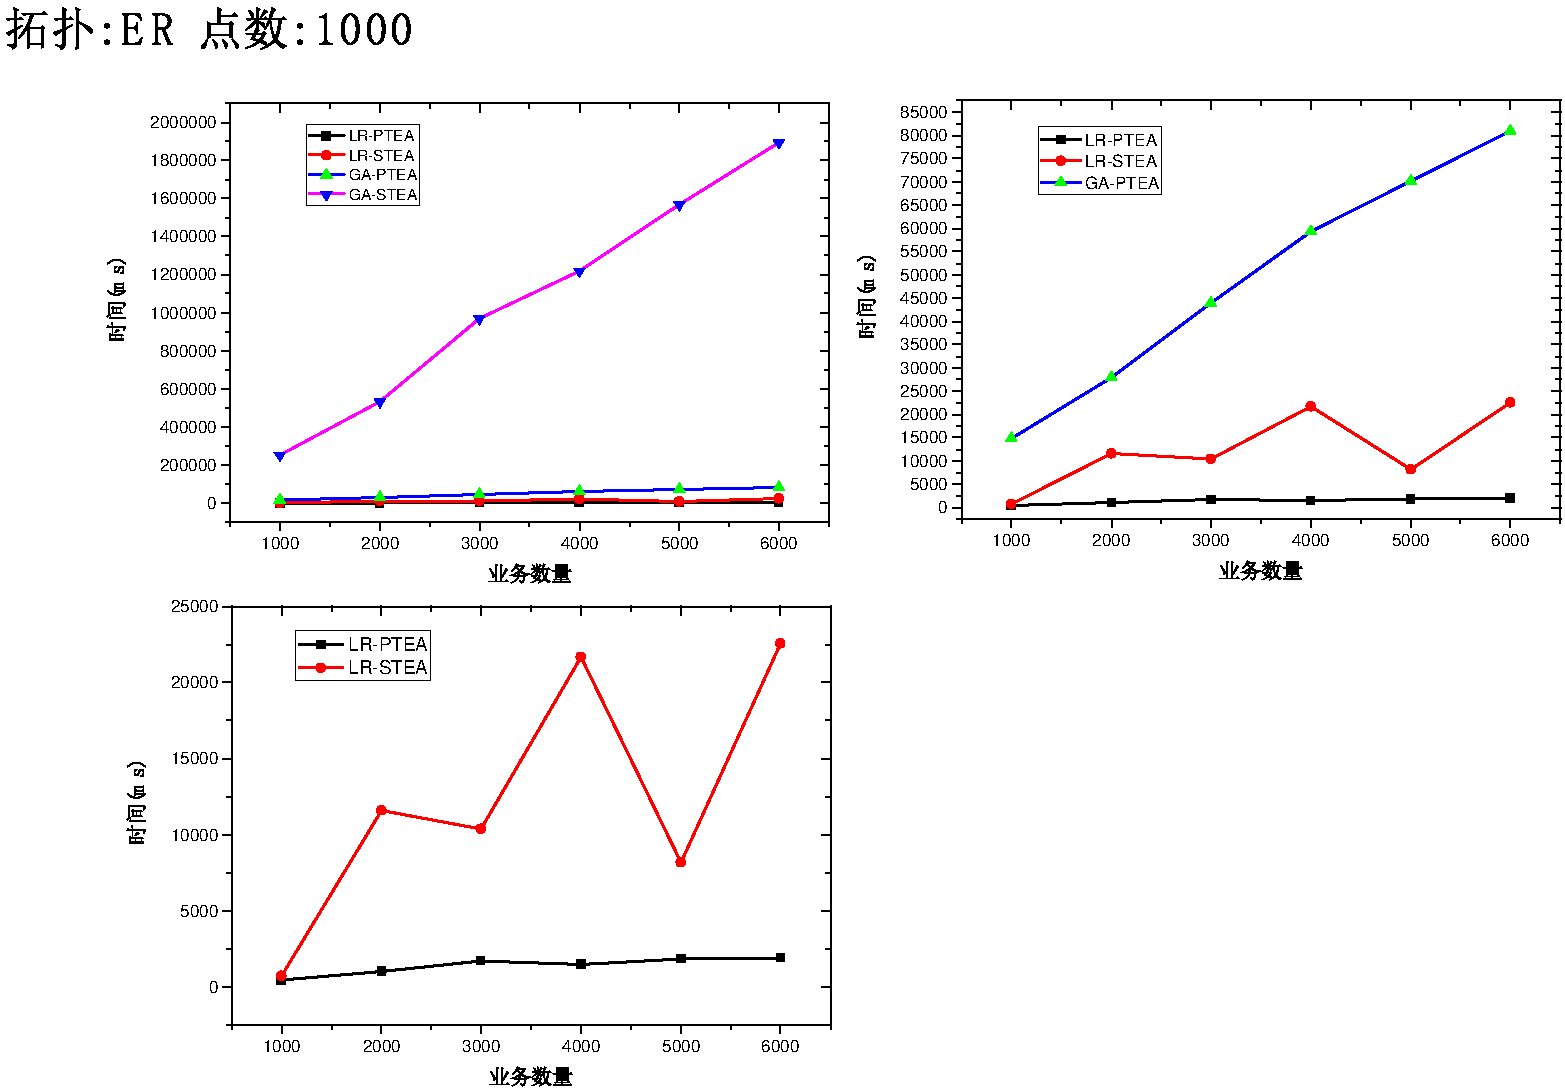
\includegraphics[width=0.8\textwidth]{figures/TI-ER-TA-1000.pdf}}
\end{center}
\caption{{\footnotesize{Time-Task(ER 1000)}}}
\label{TI-ER-TA-1000}
\end{figure}
\begin{figure}
\setlength{\belowcaptionskip}{-0.1cm}
\begin{center}
{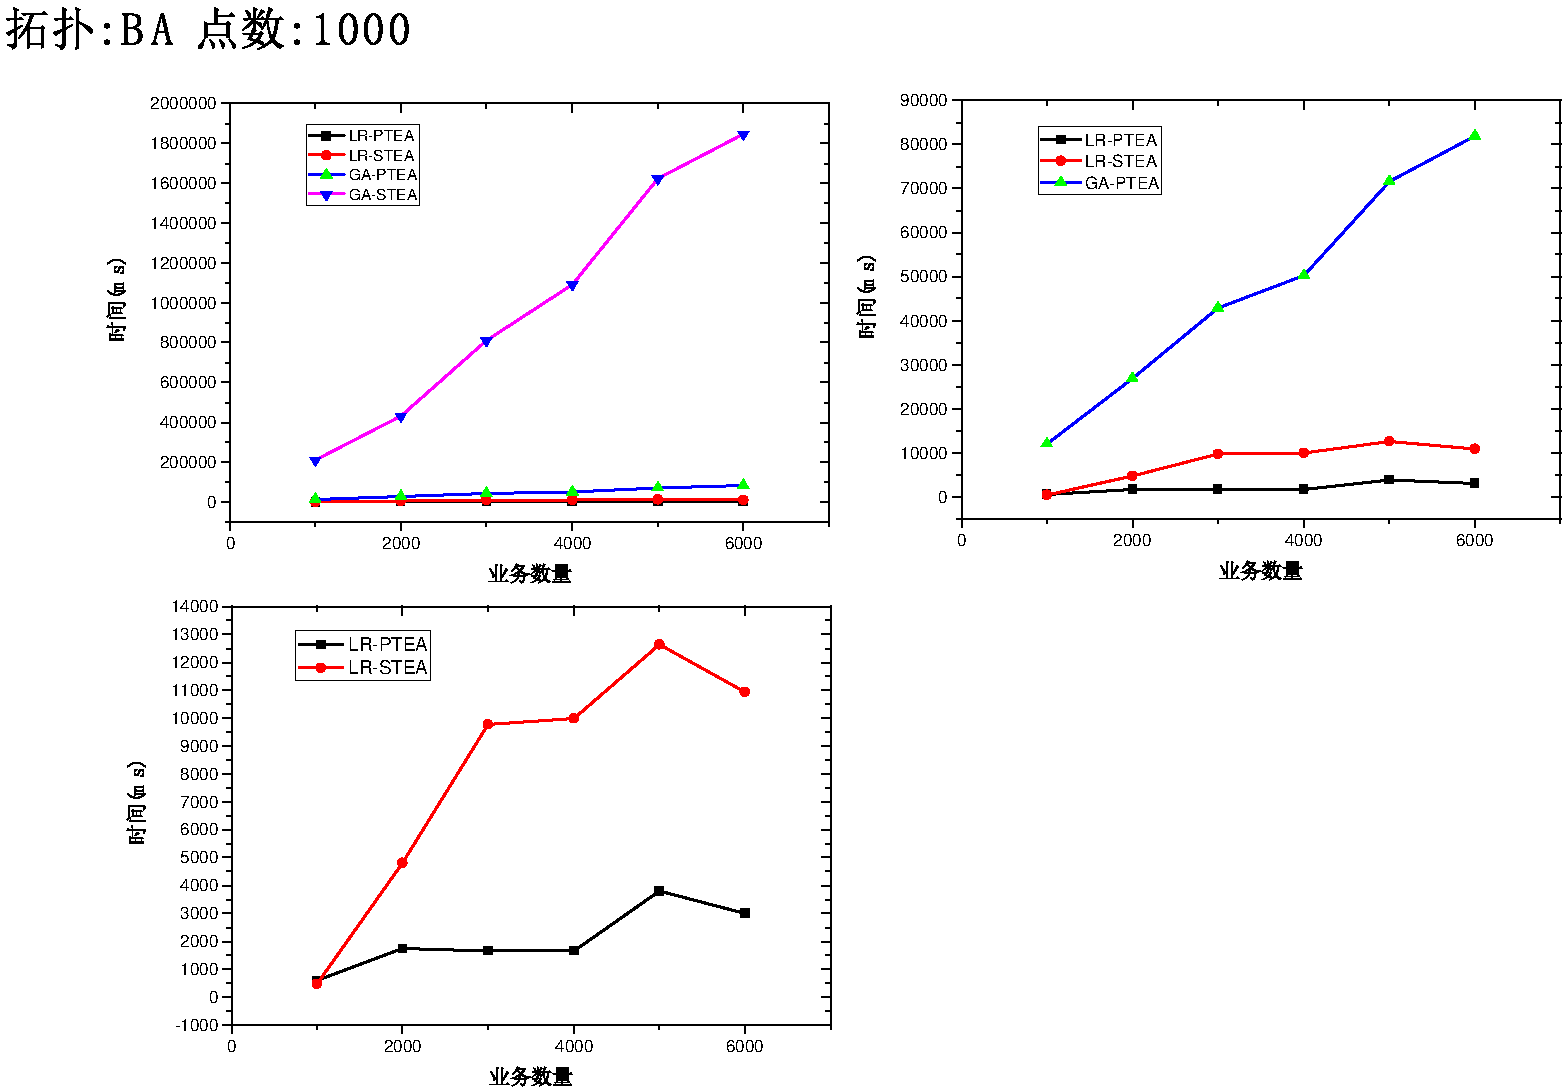
\includegraphics[width=0.8\textwidth]{figures/TI-BA-TA-1000.pdf}}
\end{center}
\caption{{\footnotesize{Time-Task(BA 1000)}}}
\label{TI-BA-TA-1000}
\end{figure}
\begin{figure}
\setlength{\belowcaptionskip}{-0.1cm}
\begin{center}
{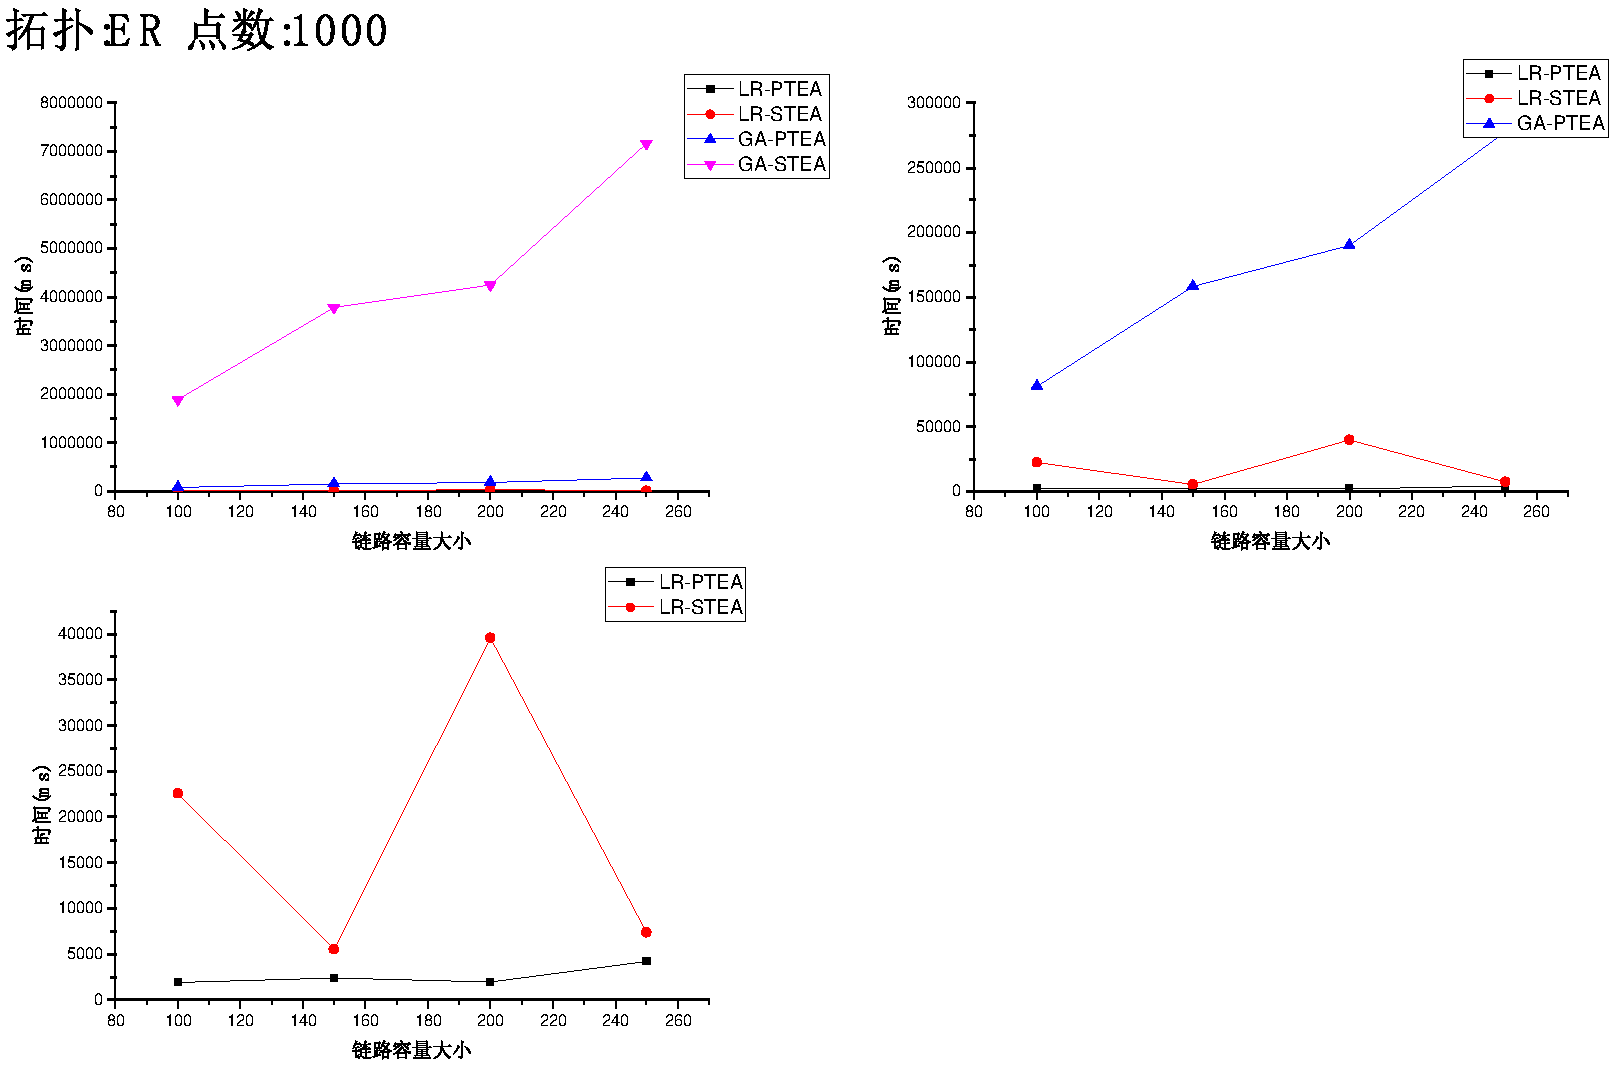
\includegraphics[width=0.8 \textwidth]{figures/TI-ER-CA-1000.pdf}}
\end{center}
\caption{{\footnotesize{Time-Capacity(ER 1000)}}}
\label{TI-ER-CA-1000}
\end{figure}
\begin{figure}
\setlength{\belowcaptionskip}{-0.1cm}
\begin{center}
{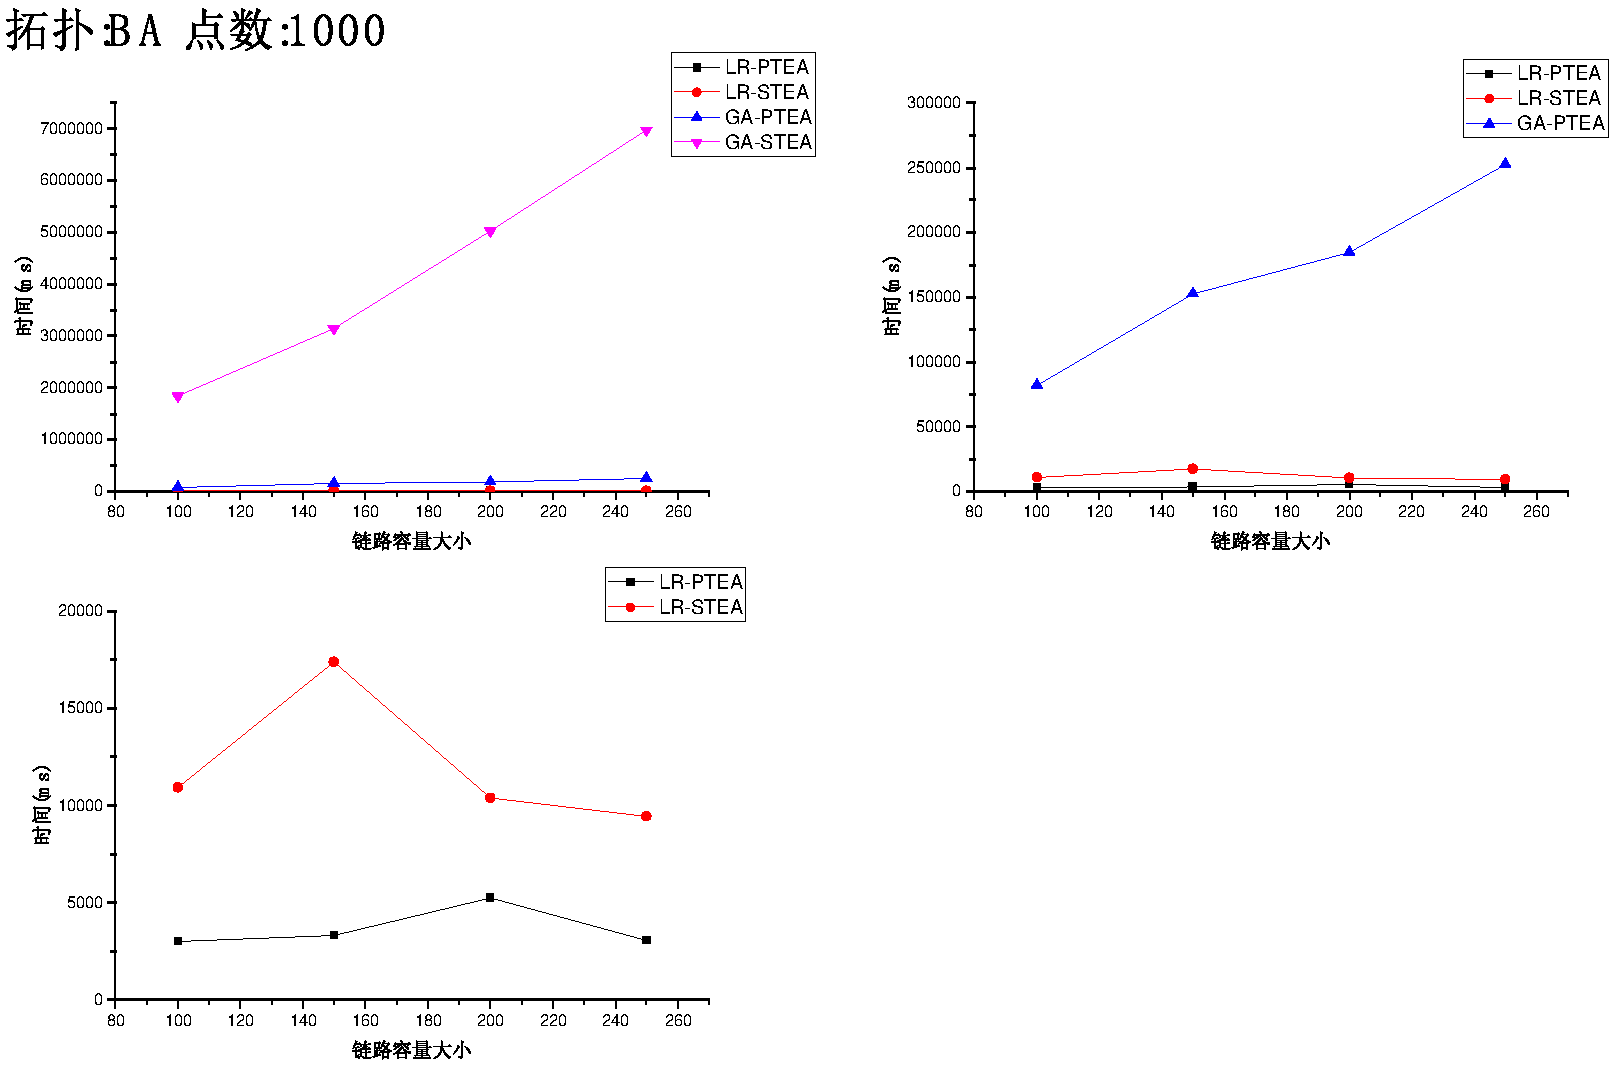
\includegraphics[width=0.8 \textwidth]{figures/TI-BA-CA-1000.pdf}}
\end{center}
\caption{{\footnotesize{Time-Capacity(ER 1000)}}}
\label{TI-BA-CA-1000}
\end{figure}
\begin{figure}
\setlength{\belowcaptionskip}{-0.1cm}
\begin{center}
{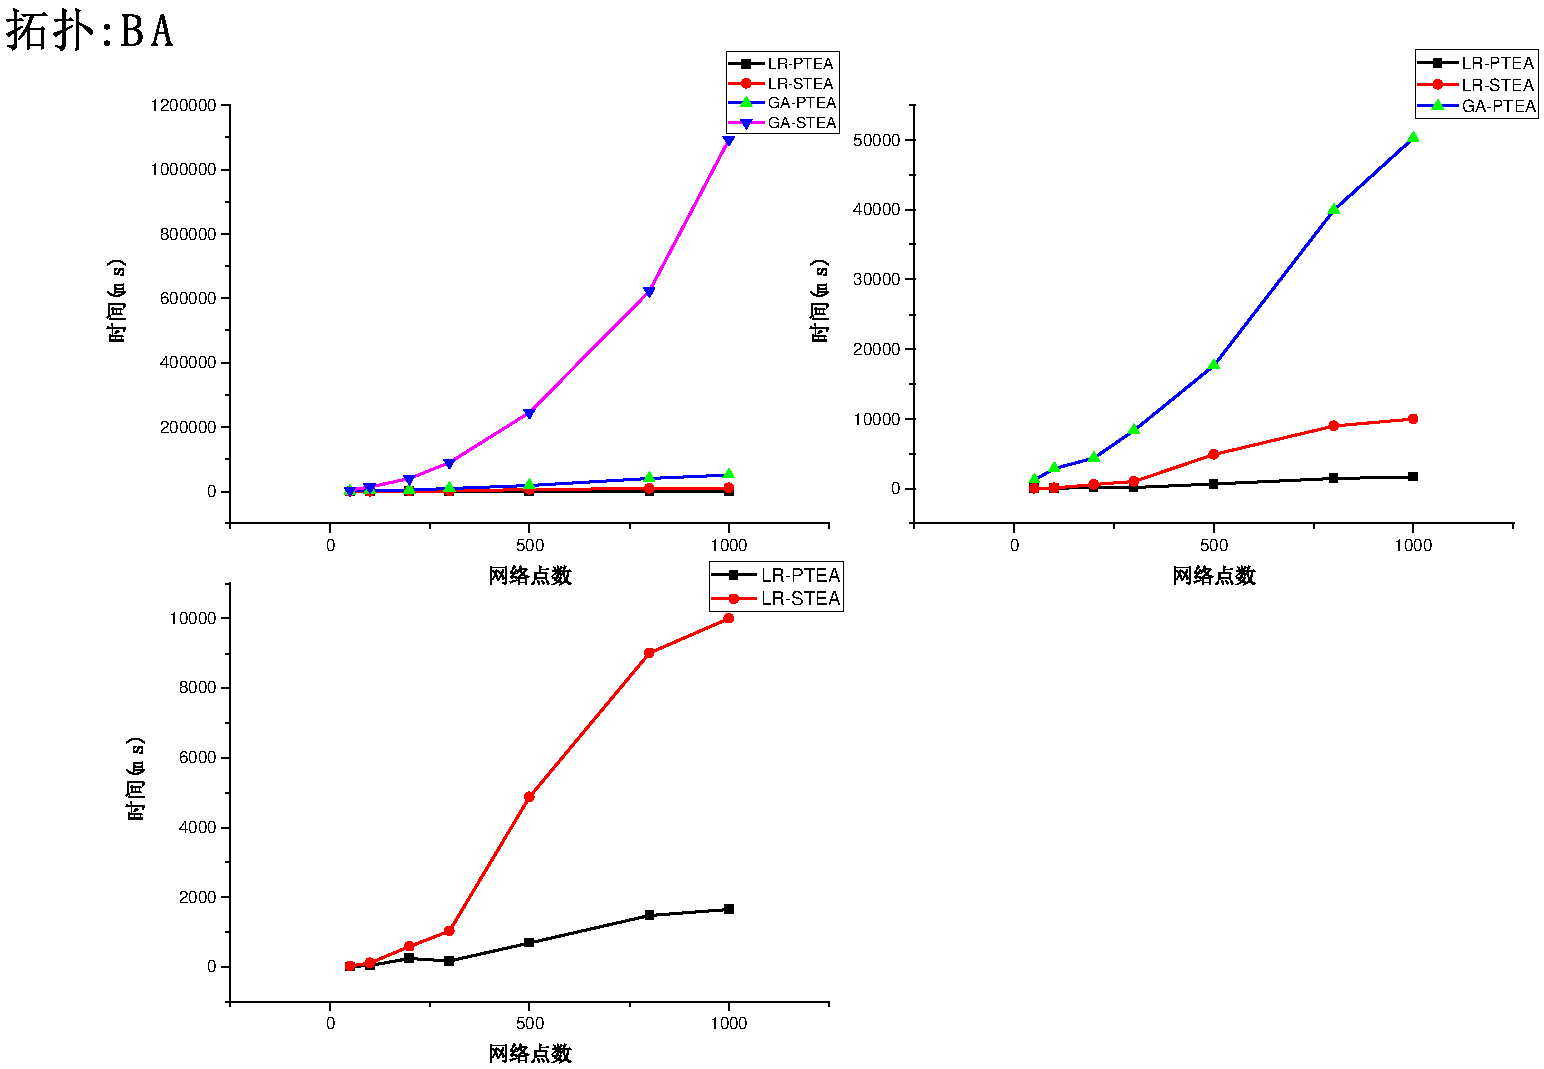
\includegraphics[width=0.8\textwidth]{figures/TI-BA-NO.pdf}}
\end{center}
\caption{{\footnotesize{Time-Node(BA)}}}
\label{TI-BA-NO}
\end{figure}
\begin{figure}
\setlength{\belowcaptionskip}{-0.1cm}
\begin{center}
{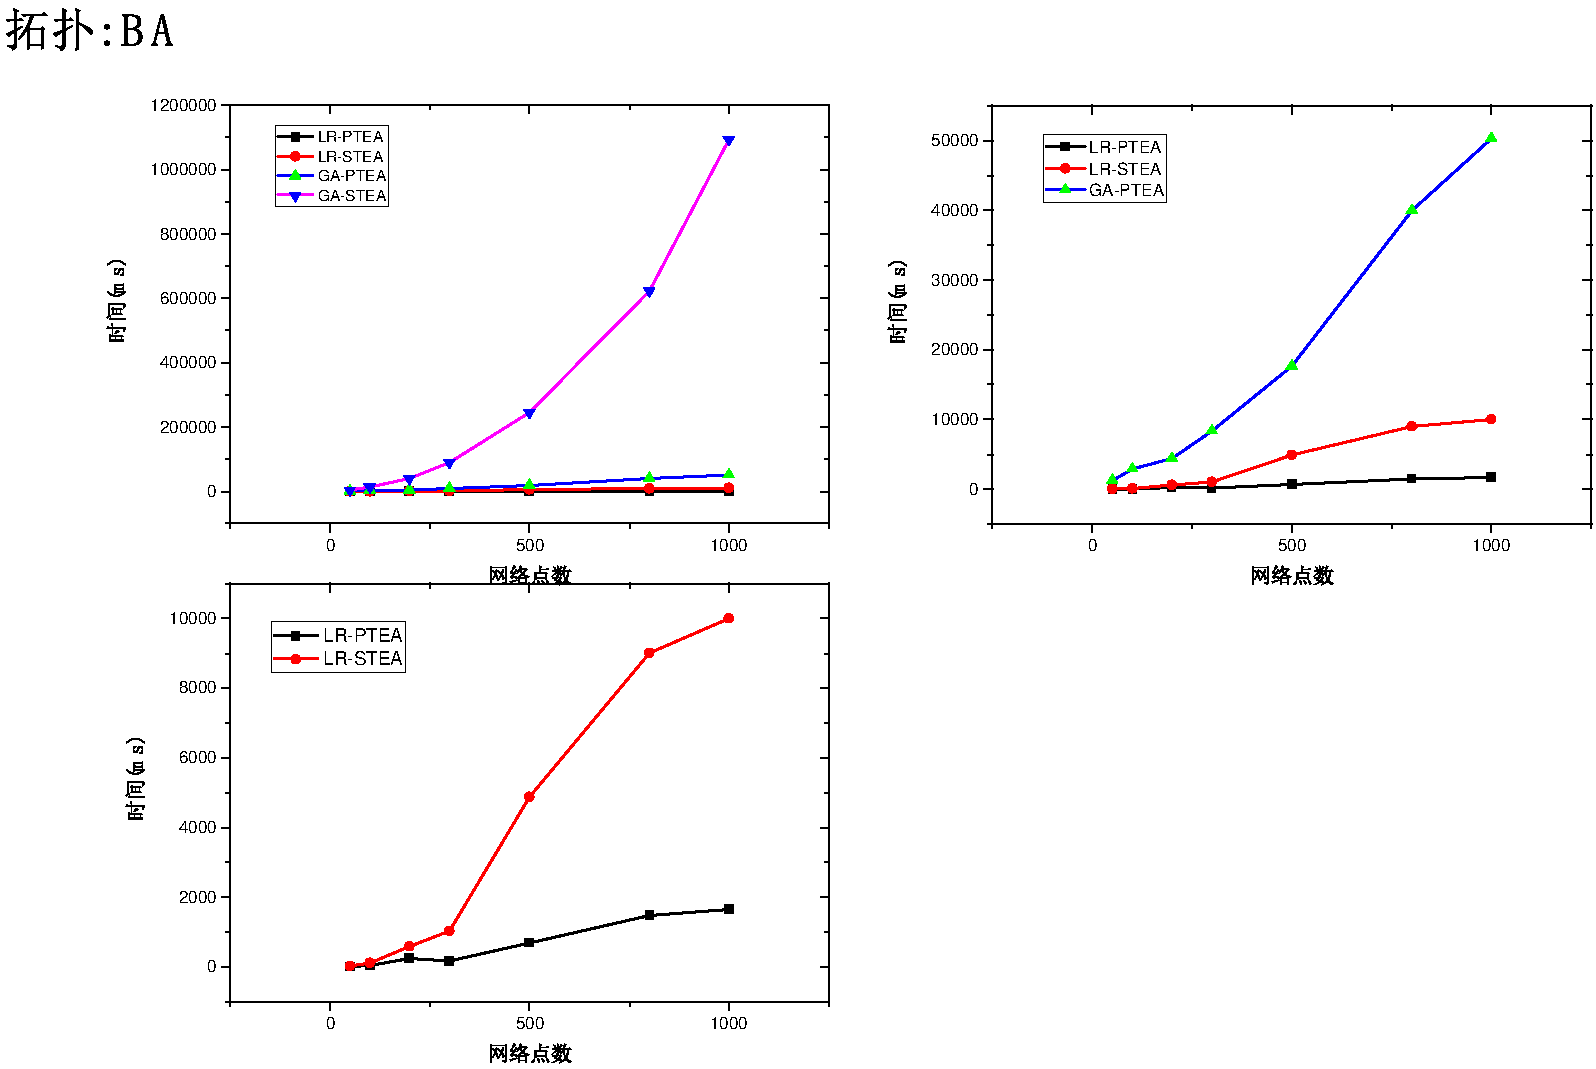
\includegraphics[width=0.8 \textwidth]{figures/TI-ER-NO.pdf}}
\end{center}
\caption{{\footnotesize{Time-Node(ER)}}}
\label{TI-ER-NO}
\end{figure}
\subsubsection{算法收敛性}
图 \ref{CO-GA-1000} 和图 \ref{CO-LR-1000} 分别是GA-PROA和LR-PROA的收敛过程图。可以看到遗传算法的初始值较差,迭代次数较多,但是最终还是陷入了局部最优解,而LR-PROA的算法第一次的值已经很好,这是因为LR-PROA不是基于备选路径的,他会通过路径调整过程为业务重新寻找路径,从而得到一个较好的初始目标值,LR-PROA算法的目标函数值在很短的迭代次数里快速下降,但是LR-PROA的曲线不够平滑,说明算法的波动很大,收敛终止条件不好控制,这也是 图 \ref{TI-ER-TA-1000}和图 \ref{TI-BA-TA-1000}产生波动的原因。
\begin{figure}
\setlength{\belowcaptionskip}{-0.1cm}
\begin{center}
{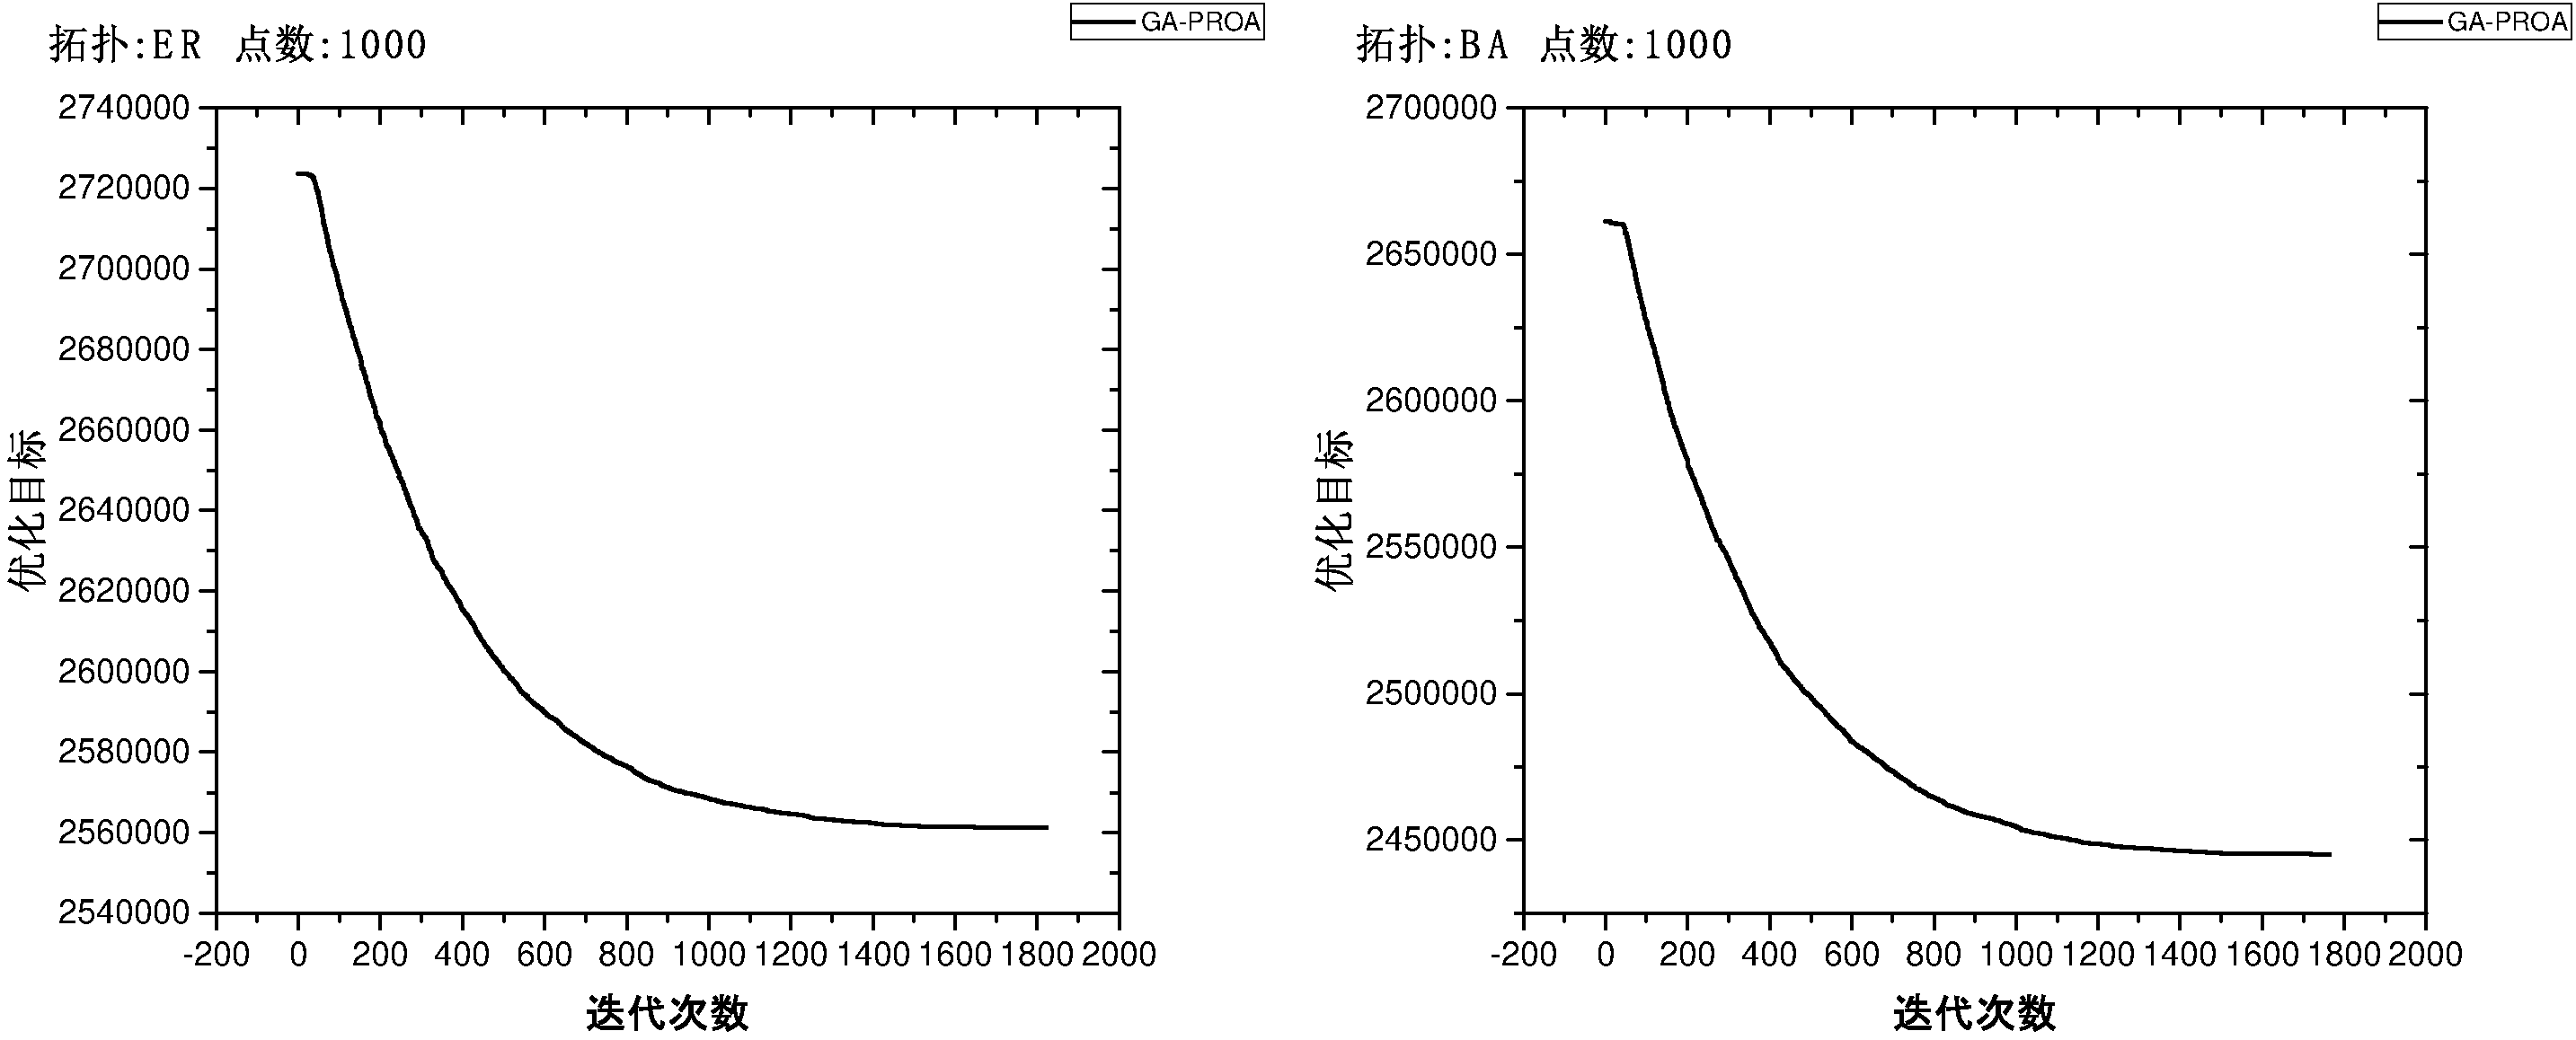
\includegraphics[width=0.8\textwidth]{figures/CO-GA-1000.pdf}}
\end{center}
\caption{{\footnotesize{GA-PROA 收敛性}}}
\label{CO-GA-1000}
\end{figure}
\begin{figure}
\setlength{\belowcaptionskip}{-0.1cm}
\begin{center}
{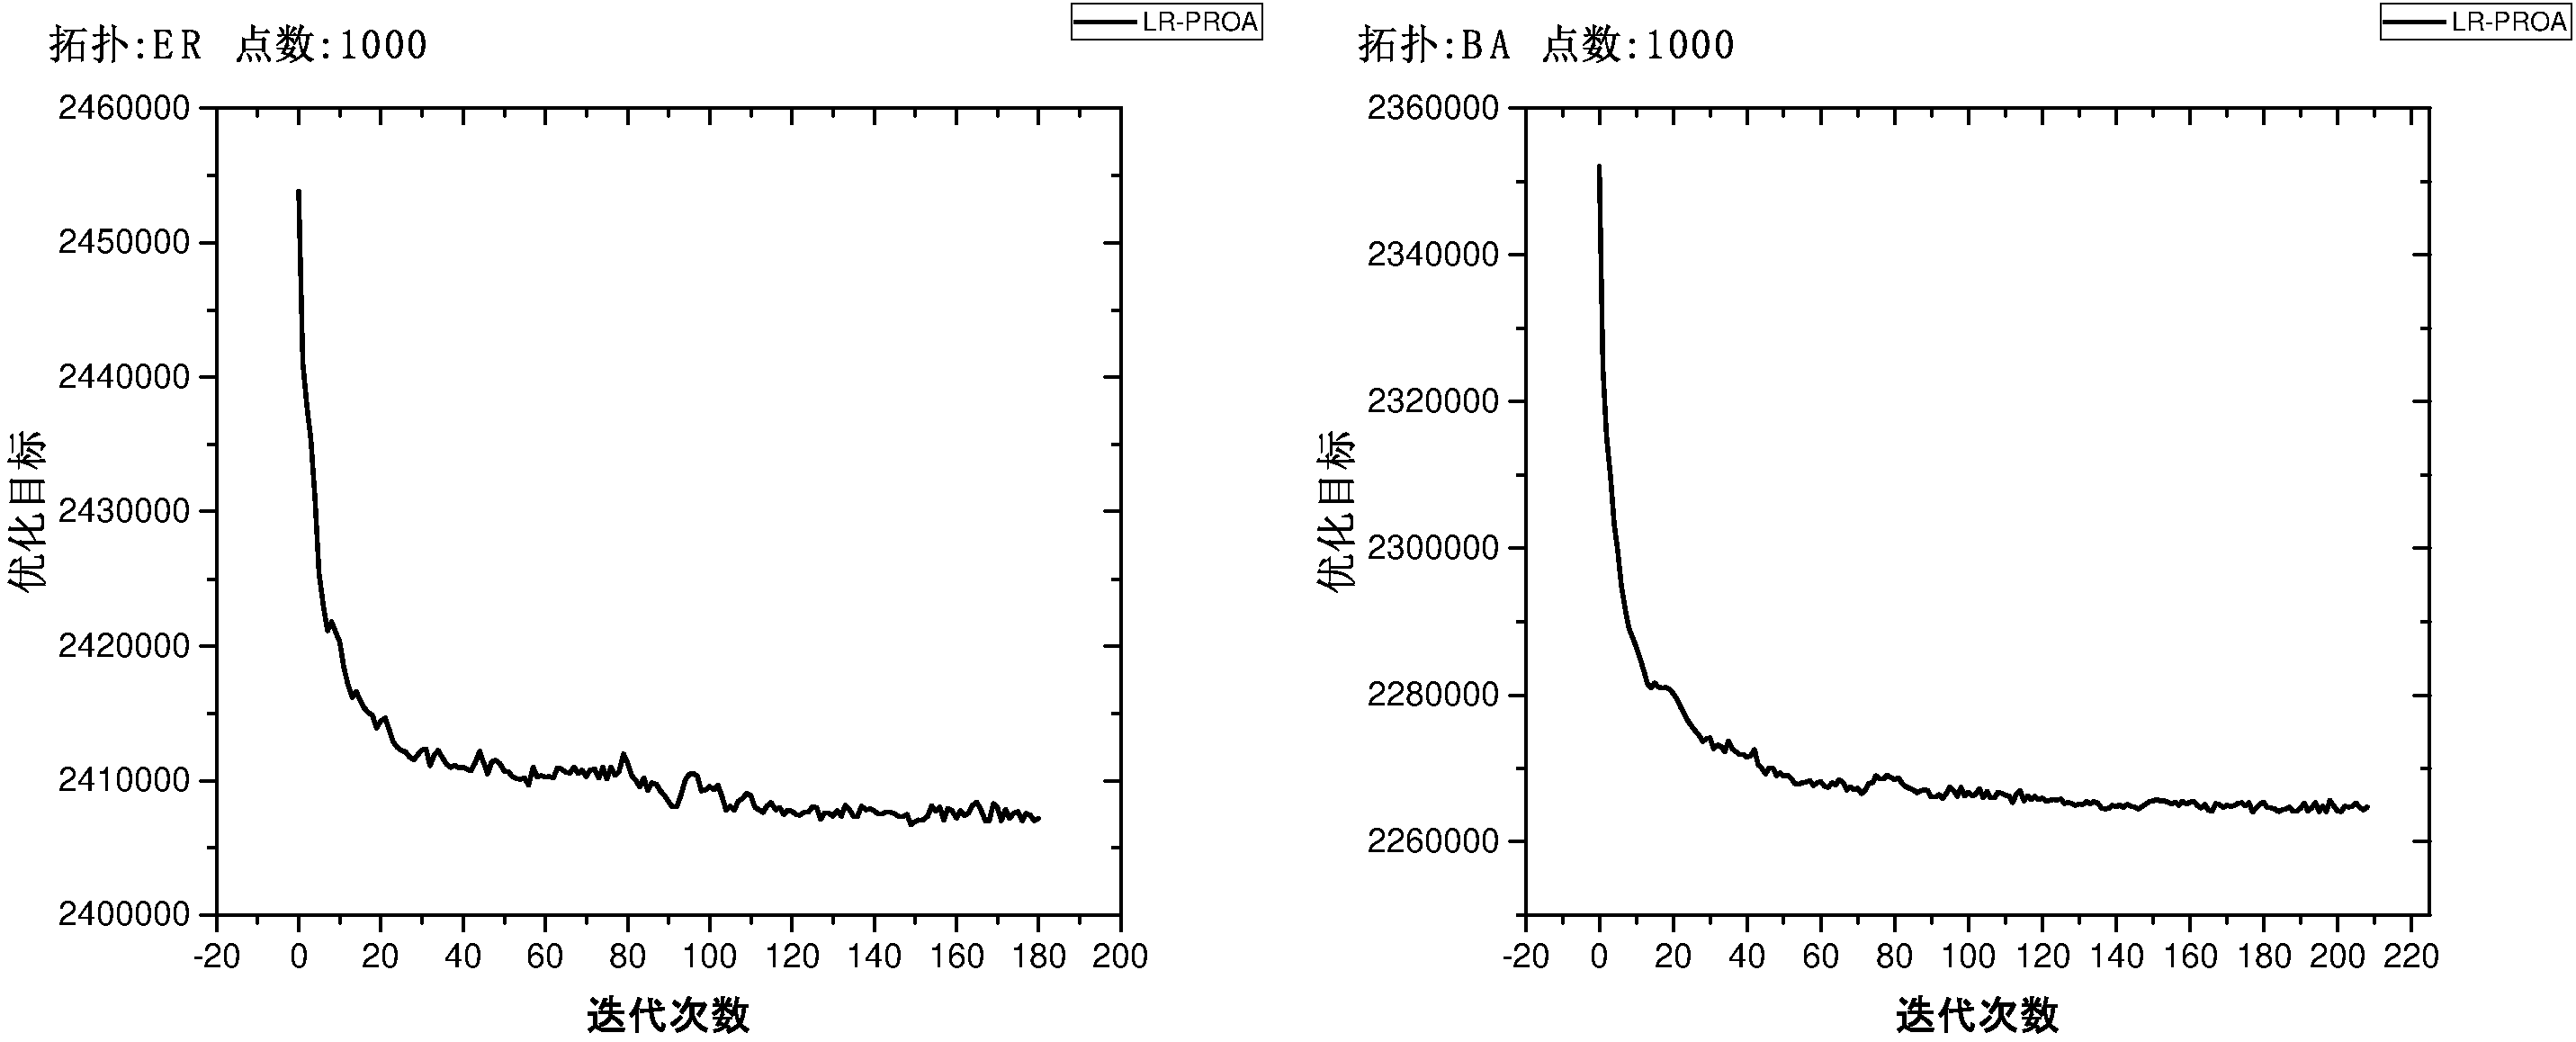
\includegraphics[width=0.8 \textwidth]{figures/CO-LR-1000.pdf}}
\end{center}
\caption{{\footnotesize{LR-PROA 收敛性}}}
\label{CO-LR-1000}
\end{figure}
\section{本章总结}
本章研究了SDN网络下的并行业务量工程算法,首先提出了新的路由优化目标函数,建立了路由优化模型,设计了两种基于GPU的并行优化算法方案GA-PROA和LR-PROA,最后,进行实验,发现GA-PROA能够加速10-20倍,LR-PROA能够加速达到6倍,LR-PROA能够在短时间内得到目标函数的优化解。







